\documentclass[10pt, a4paper]{article}
\usepackage{color}
\usepackage{graphics}
\usepackage{graphicx}
\usepackage[numbers]{natbib}
\usepackage{calc}
\usepackage{longtable}
\usepackage[svgnames,table]{xcolor}
%\usepackage[table]{xcolor}
\usepackage{paralist}
\usepackage{fancyhdr}
\pagestyle{fancy}
\usepackage{fancyheadings}
\topmargin = 1pt
\headheight=10mm
\headsep=7pt
%\ensuremath
\usepackage{lastpage}
\usepackage{float}
\usepackage{subfig}
\usepackage{caption}
\usepackage{appendix}
\captionsetup{margin=10pt,font=small,labelfont=bf}
\usepackage{wrapfig}
\definecolor{darkblue}{rgb}{0.0,0.0,0.3}
\setcounter{tocdepth}{4}
\parindent 0pt
%\floatstyle{boxed} 
\restylefloat{figure}
\usepackage[a4paper=true, ]{hyperref}

%%%%%%%%%%%%%%%%%%%%%%%% End Document Setup %%%%%%%%%%%%%%%%%%%%%%%%%%%%

%%%%%%%%%%%%%%%%%%%%%%%%% Begin Lemenkova Polina's MSc Thesis Document%%%%%%%%%%%%%%%%%%%%%%%%%%

\begin{document}

\pagenumbering{roman}

\title{Seagrass mapping and monitoring along the coasts of Crete, Greece}
\author{by Lemenkova Polina}
\date{\today}
\maketitle
\pagebreak

\textbf{Course Title:} \hfill{Geo-Information Science and Earth Observation for Environmental Modelling and Management}\\


\textbf{Level} \hfill{Master of Science (MSc)}\\
\textbf{Course Duration:} \hfill{September 2009 – March 2011}\\
\textbf{Consortium partners:} \\


University of Southampton (UK)\\
Lund University (Sweden)\\
University of Warsaw (Poland)\\
University of Twente, Faculty ITC (The Netherlands)

\pagebreak

\begin{center}
\textbf{Seagrass mapping and monitoring along the coasts of Crete, Greece}\\
 {by Lemenkova Polina}
\end{center}

Thesis submitted to the University of Twente, faculty ITC, in partial fulfilment of the requirements
for the degree of Master of Science in Geo-information Science and Earth Observation for
Environmental Modelling and Management.\\

Thesis Assessment Board:\\

Name Examiner 1 (Chair)
Name Examiner 2
External Examiner
Member
Supervisors: Venus V. (Department of Natural Resource, ITC)
Toxopeus A.G. (Department of Natural Resource, ITC)\\

\begin{figure}[b]
	\begin{center}
	
\includegraphics[height=2cm,width=8cm]{ITC-logo.jpg}
	\end{center}
\end{figure}

\pagebreak

\begin{abstract}
\end{abstract}

\pagebreak
\textbf{Disclaimer}\\

This document describes work undertaken as part of a programme of study at the University of
Twente, Faculty ITC. All views and opinions expressed therein remain the sole responsibility of
the author, and do not necessarily represent those of the university.\\

\pagebreak

\section*{}
\markright{Table of Content}
\addcontentsline{toc}{section}{Table of Content}
\tableofcontents 

\textbf{Software and utilities used in the current work}:\\
\begin{itemize}
\item \href{http://www.esri.com/software/arcgis/index.html}{ArcGIS 10.0}: mapping, data integration and spatial analysis
\item \href{http://www.erdas.com/products/ERDASIMAGINE/ERDASIMAGINE/Details.aspx}{Erdas Imagine}: imagery processing and classification
\item WASI Water Color Simulator, for modelling optical water properties under changing environment
\item \href{http://welcome.hp.com/country/us/en/prodserv/handheld.html}{iPAQ} and GPS for data capture during the fieldwork
\item \href{http://www.bibtex.org/de/}{BibTeX}, for management of bibliography and reference database
\item \href{http://www.latex-project.org/}{\LaTeX}, for document typesetting, formatting and performing pdf output
\item \href{http://www.python.org/}{Python language}, for writing auxiliary scripts (e.g. raw data interpolation)
\item \href{http://www.gnuplot.info/}{Gnuplot} for plotting graphs
\item \href{http://www.openoffice.org/}{Open Office} : document typesetting, data preprocessing and preliminary statistical evalution
\item \href{http://calc2latex.sourceforge.net/}{Calc2LaTeX} : converting spreadsheets into \LaTeX environment
\item \href{http://www.spss.com/}{SPSS (PASW Statistics 18)} : statistical data edition and analysis 
\end{itemize}
\pagebreak

\section*{}
\markright{List of Figures}
\addcontentsline{toc}{section}{List of Figures}
\listoffigures
\pagebreak

\section*{}
\markright{List of Tables}
\addcontentsline{toc}{section}{List of Tables}
\listoftables
\pagebreak

\pagenumbering{arabic}
\rfoot{MSc Thesis\\ \emph{"Seagrass mapping and monitoring along the coasts of Crete, Greece"}}
\section{Introduction}
%\markright{I. Introduction}

\subsection{Summary}
The seagrasses, a unique group of aquatic plants growing submerged in the sea water, with root-like
structures (rhizoms) buried in the sediments and vertical elongate leaves. A flowering plant,
completely adapted to marine environment, they are however, more closely related to the lily family
(Liliaceae) than to true grass, despite their name “seagrass”, caused by the ribbon-like, grassy leaves
\cite{McKenzie08}\label{McKenzie08}.\\
Seagrasses create unique, complex, extremely diversified and productive ecological systems in the
littoral coastal zones between 0-50 meters in shallow waters all over the world \cite{Hogarth07}\label{Hogarth07}, and
serve as a valuable environmental indicators for the marine ecosystems health. Seagrasses are closely
connected and linked with complex interactions to other vegetation types, e.g. mangroves, coral reefs,
etc. An important constructing component of littoral ecosystems, seagrass contributes significantly to
their structure and functioning.\\
The adaptation to the salt waters is evidently influenced the global ditribution of the seagrasses,
limiting it to shallow coastal areas. A number of critical conditions determines grouth of seagrass,
including general climatic characteristics of the area, i.e.temperature, day length, geological and
geomorphological conditions, e.g. soft type of sediments (sand or mud), shallow depths, as well as
chemical and physical parameters of the water: salinity, waves \cite{McKenzie02}\label{McKenzie02}.
The seagrass Posidonia oceanica (further \textit{P.oceanica}) is a key species to inhabit littoral of the
Mediterranean Sea, see Fig. \ref{fig:1}

\begin{figure}[h]
	\centering
	\subfloat {\label{fig:1-1a}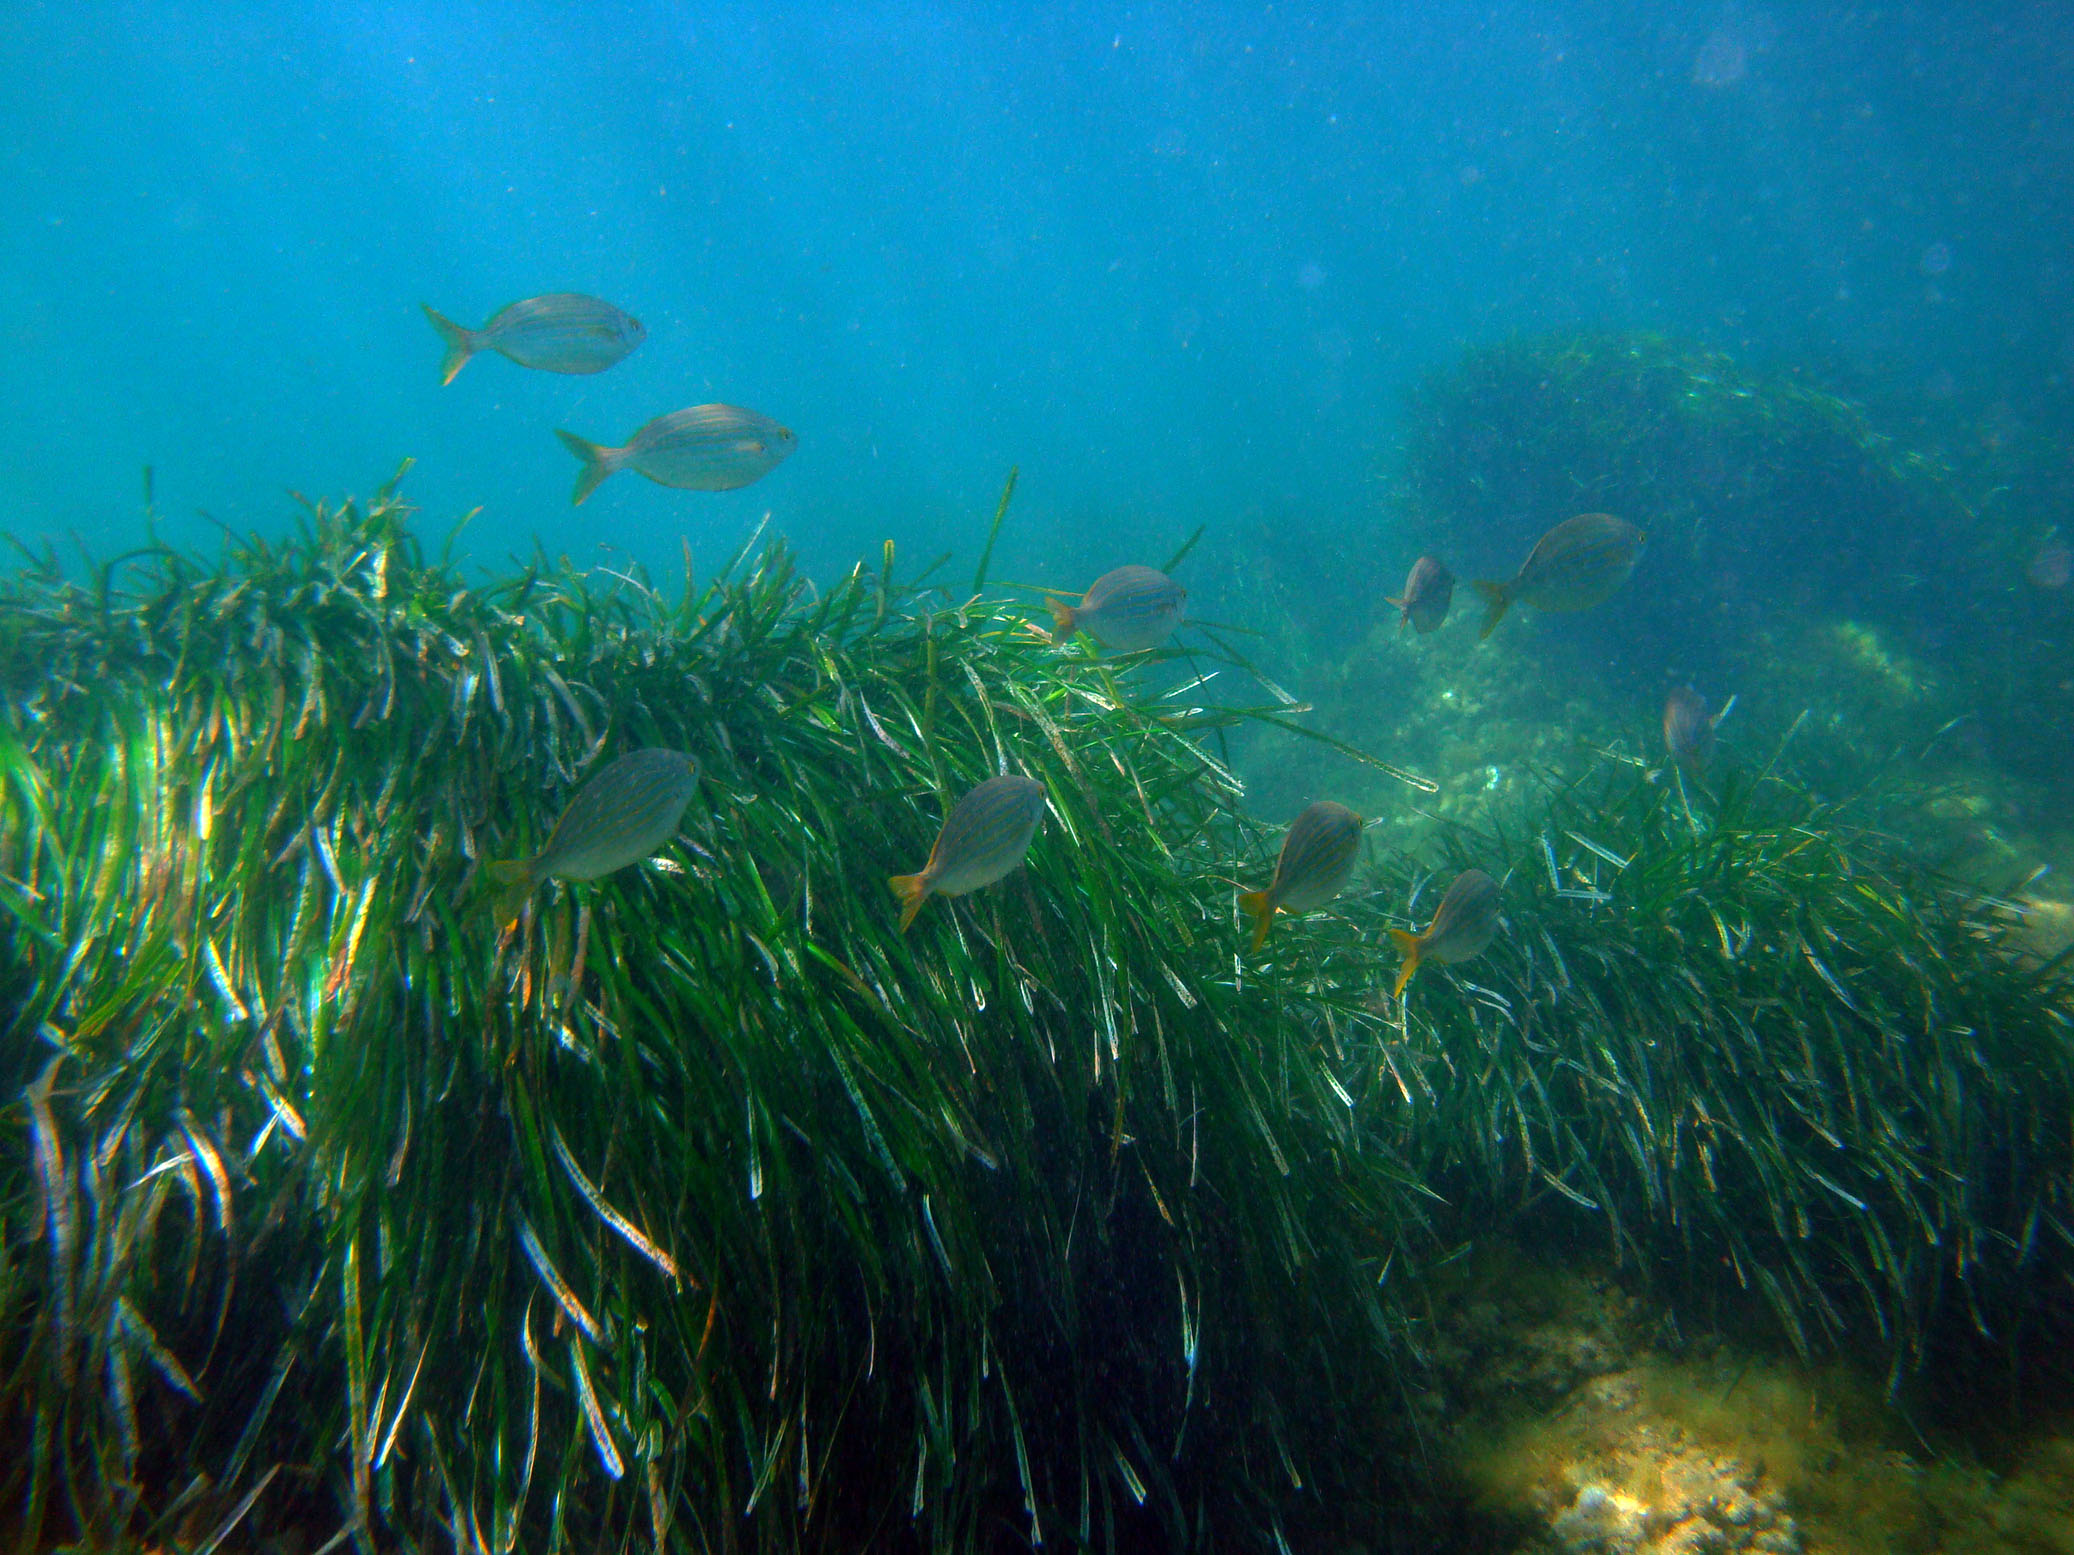
\includegraphics[width=0.4\textwidth]{Fig-1-1a.jpg}}
	\hspace{2mm}
	\subfloat {\label{fig:1-1b}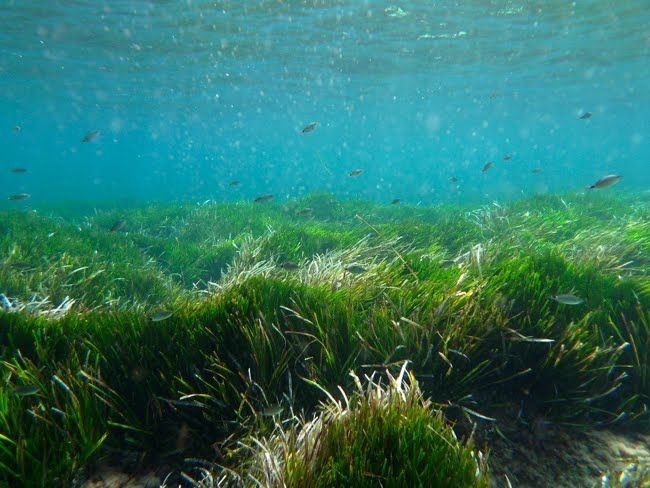
\includegraphics[width=0.4\textwidth]{Fig-1-1b.jpg}}
	\caption{Seagrass Posidonia Oceanica}
	\label{fig:1}
\end{figure}

and is widely spread along the coasts of Crete \cite{Dumay02} \label{Dumay02}. 
It plays an important role in a number
of geomorphological and ecological processes. Namely, it is a source of food for herbivorous fauna as
well as helter zones for fish and other marine organisms; it contributes to the nutrient recycling; it
provides sediments stability by reducing the degree of water movements, etc \cite{Francour99}\label{Francour99}.\\
The purpose of current MSc research work aims to apply methods of remote sensing and GIS
including processing and classification of satellite, aerial photos and videometric underwater imaging
as well as GIS-based spatial analysis towards mapping and environmental monitoring of \emph{P. oceanica}
along the coasts of Crete island, Greece. The technical implementation is based on ENVI, Erdas
Imagine, WASI and ArcGIS software using aerial and satellite images as well as results of the
underwater videometric measurements.

\subsection{Background}
\subsubsection{Global distribution of the seagrasses}
Globally, there are 58 recognized and described seagrass species \ref{fig:2}, belonging to two orders
(Hydrocharitales and Najadales), four families (Hydrocharitaceae, Posidoniaceae, Cymodoceaceae
and Zosteraceae), and 12 genera (Enhalus, Thalassia, Halophila, Posidonia, Syringodium, Halodule,
Cymodocea, Amphibolis, Thalassodendron, Zostera, Heterozostera and Phyllospandix) \cite{Kuo89}\label{Kuo89}.
\begin{wrapfigure}{r}{0.4\textwidth}
\centering
	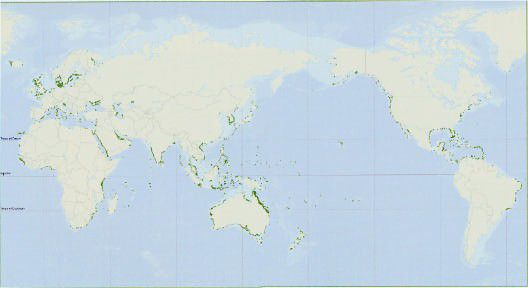
\includegraphics[scale=0.25]{Fig-1-2.jpg}
	\caption{Distribution of seagrasses in the world.\\ Source:\cite{Green03}\label{Green03} \label{fig:2}} 
\end{wrapfigure}
The distribution of the seagrasses is strongly influensed by several environmental factors, which
include climate (mostly, tropical and temperate areas), bathymetry (shallow shelf zones), hydrological
particularities (chemical content of water, nutritient availability and turbidity of waves), and geological 
characteristics - sedimentation and cover types of the seafloor \cite{McKenzie06}\label{McKenzie06}.\\
There are four European seagrass species in Mediterranean area \cite{Borum04}\label{Borum04}: Zostera marina,
Zostera noltii, Cymodocea nodosa and \textit{P.oceanica}. In Greece the common species are\textit{P.oceanica}
(L.) Delile, Cymodocea nodosa (Ucria) Ascherson, Zostera noltii Hornemann and Halophila
stipulacea \cite{Amoutzopoulou-Schina05}\label{Amoutzopoulou-Schina05}. 
These species differ in morphological and
phenological features (Fig. \ref{fig:3}) as well as in structure and dynamics. Thus, Cymodocea nodosa is
considered the pioneer species of \textit{P.oceanica} beds, the latter species forming the last stage. When P.
oceanica beds regresses, C. nodosa often replaces them \cite{DenHartog77}\label{DenHartog77}; as a result, \textit{P.oceanica},
C. nodosa, and Z. noltii do not form mixed persistent stands \cite{Buia91}\label{Buia91}.

\subsubsection{Ecological significance of the seagrasses}
Seagrass plays vital role in the marine ecosystems of the world ocean. Seagrasses are the only
flowering plant in the world that is able to live completely submerged. Seagrass is a habitat for
numerous marine fish species \cite{Nagelkerken00}\label{Nagelkerken00}, source of primary production and food for
fish, turtles and other organisms, which gives them special environmental value \cite{Noralez10}\label{Noralez10}.\\
Seagrass meadows produce enormous quantities of organic matter (leaves, epiphytes), which
constitutes the basis of the food web both within and outside the ecosystem \cite{Gobert06}\label{Gobert06}.

\begin{wrapfigure}{r}{0.4\textwidth}
\centering
	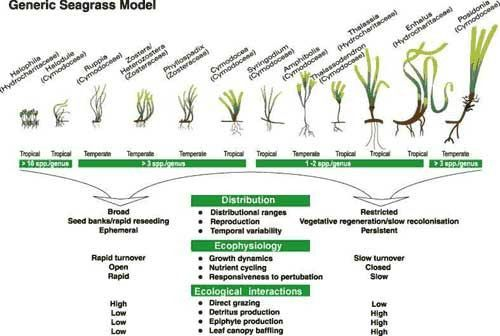
\includegraphics[scale=0.25]{Fig-1-3.jpg}
	\caption{Morphology of different types of seagrasses.
	\label{fig:3}
Source: \url{http://www.ozcoasts.org.au}}
\end{wrapfigure}

Finally, seagrasses are an important component in the environmental "food chain" of the coastal
ecosystems, being the food source for dugongs, turtles, swans and various fish \cite{Cappo95}\label{Cappo95}.\\
Due to their wide distribution, meadows size, easy collection and abundance, sensitivity to the
modifications of the coastal zone and their important role in maintaining coastal water quality
and clarity, seagrass is perfect indicator and descriptor of the environmental health of marine
ecosystems, and is highly suitable for the environmental monitoring \cite{Pergent-Martini05}\label{Pergent-Martini05}.\\
Being often confused with marine “algae”, “seagrasses” are vastly different from them. There are
fundamental differences between both marine organisms, the major of them should be briefly
mentioned: first, seagrasses are true plants with root system and leaves which photosynthesise, have
complex structure and create landscape-similar vast formations on the colonised seafloor areas with
soft sediment, whereas algae are simple organisms that can only holdfast; secondly, seagrasses are
complex vascular plants with reproductive mechanism such as fruits, seeds and spores, while algae
have simple few cell structure with spores and gametes; finally, seagrasses uptake nutrient through
root system, while algae nourish directly from the water column \cite{Dixon05}\label{Dixon05}. There are other
differences between “seagrass” and “algae” but they go beyond the scope of this work.

\subsubsection{Environmental vulnerability of the seagrasses}
Meadows of P. oceanica are subjected to the human activities, as they occur in coastal areas, where
they can be affected both directly \cite{Meinesz91}\label{Meinesz91} or indirectly, through the impact on the
quality of waters and sediments \cite{Duarte02}\label{Duarte02}. As \textit{P.oceanica} is a long-living plant with a slow
growth rate, the anthropogenic modifications of the coastal zone, happening more rapidly than the
capacity of the plant to adapt to these changes, reduce its distribution area \cite{Micheli05}\label{Micheli05}. One
of the main drivers of seagrass decline is, for instance, the location of the fish farming near the
seagrass meadows. The negative effects of the sedimentation of waste particles in the farm vicinities
on \textit{P.oceanica} meadows are diverse and complex, and may cause benthic deterioration, accumulation
of organic matter and seagrass decline \cite{Holmer08}\label{Holmer08}. Seagrasses are subject to anthropogenic
nutrient (N and P) loading, which may occasionally casue morphological (e.g. leaf length) and
physiological (e.g. chlorophyll and nitrogen content of the leaves) responses towards changed
environmental conditions \cite{Leoni06,Leoni07}\label{Leoni06} \label{Leoni07}. 

\begin{wrapfigure}{r}{0.5\textwidth}
\centering
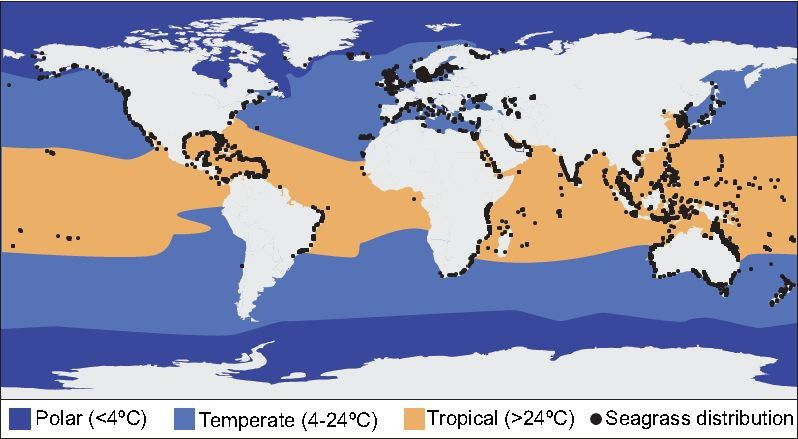
\includegraphics[scale=0.20]{Fig-1-4.jpg}
\caption{Distribution of seagrass in relation to mean
ocean temperature. \\
Source: \cite{Orth06}\label{Orth06}}
\label{Fig.4}
\end{wrapfigure}

The detailed research of the fish
farm-induced decline of the seagrass meadows \cite{Diaz-Almela06}\label{Diaz-Almela06}reports the relationships of
fish farm organic and nutrient content in the sediments with dynamics of the key seagrass species (P.
oceanica) in the Mediterranean Sea. Nowadays P.oceanica is in the alarming state of regression due
to the deterioration of the environment in the Mediterranean Sea \cite{Ribed02}\label{Ribed02}. Due to these reasons,
\textit{P.oceanica} is a protected species since 1988 in some European countries \cite{Francour99}\label{Francour99}, and
its presence serves as an indicator of a stable healthy environment. Among other negative factors,
affecting both growth and status of the seagrasses the environmental contaminants can be mentioned,
e.g. thermal, sewage, dredging and chemical pollution as well as any other kind of maritime works,
e.g. trawling and anchoring of boats \cite{Ribed02}\label{Ribed02}. Other human activities that cause degrading of the
seagrass are recreational boating, commertial overexploitation of coastal resources, eutrophication
\cite{McKenzie06}\label{McKenzie06}.\\
Besides anthropogenic factors, various biochemical, climatic and environmental processes can cause
negative influence on seagrass distribution. Seagrass is exposed to threats from the global climate and
environmental change, i.e. increases in sea surface temperature; sea level rise; increased frequency
and intensity of storms and waves; local decrease of water quality, increased sedimentation,
contaminantion and nutrification; desiccation; salinity fluctuations; nutrient changes; suspended
sediments \cite{Blake00}\label{Blake00}. These stress-drivers can alone result in large-scale seagrass
degradation, but often seagrass undergo simultaneous affects from several of these factors together.
This naturally increase environmental pressing and leads to drastical loss of very large areas of
seagrass globally \cite{Orth06}\label{Orth06}.
In tropical areas, where most of seagrasses are located (Fig.\ref{Fig.4}), seagrasses are subject to catastrophic
extinction and loss, due to the cyclones, typhoons, storms, regular floods and increased rainfalls. Recovery from such
events can take up to several years and often it is only possible by means of the seed reserves from the local
environmental surveys \cite{McKenzie07}\label{McKenzie07}. Other threats for seagrasses in tropical areas are 
increased nutrient availability in the coastal zones, increased
eutrophication and invasive macroalgae. These processes have strong affect on the status of the
seagrass meadows, and often lead to their complete disappearance \cite{Holmer09}\label{Holmer09}.
Other environmental threat for the seagrasses arise as a result of the environmental struggle and
competition for existence among species. Thus, meadows of P.oceanica in the Mediterranean Sea are
presently facing invasion by alien algal species, partuicularly in areas where P.oceanica is already
degrading, stressed, have gaps and patchy structure in meadows and show other signs of regression
\cite{Montefalcone10}\label{Montefalcone10}.
Seagrasses are vulnerable fragile species, important for the marine coastal ecosystems, especially for
the protection of the beach structure. However, the facts about seagrass global degrading sound
worrying: about 54 percent of the total seagrass meadows have lost any part of their area; the areas, where
the seagrass ecosystems are degrading or lost, are not located in a specific area or continent, but
registered globally; since 1980s global losses of the seagrases on our planet is equal to two footbal
fields per hour \cite{Mellors09b}\label{Mellors09b}.

\subsubsection{General characteristics of Posidonia oceanica}
The endemic Mediterranean seagrass Posidonia oceanica (further \textit{P.oceanica}), is a main species in
marine coastal environment of Greece, forming, despite its slow growth, the largest, most widespread,
homogeneous and dense meadows in the Mediterranean between 5 and 40 m depth \cite{DenHartog70}\label{DenHartog70}.

\begin{wrapfigure}{r}{0.5\textwidth}
\centering
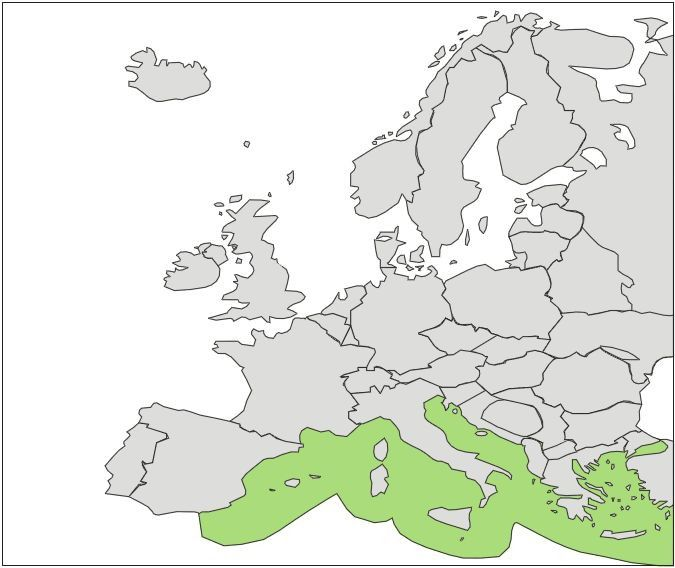
\includegraphics[scale=0.20]{Fig-1-5.jpg}
\caption{Geographical distribution of
\textit{P.oceanica}. Source: \cite{Borum04}\label{Borum04}}
\label{fig:5}
\end{wrapfigure}

The dominant and most productive coastal ecosystem of the Mediterranean, P.oceanica is
spatially restricted to the Mediterranean area (Fig.\ref{fig:5}), with its extention limited by the western part
of the Mediterranean Sea where cold Atlantic waters enter Gibraltar and mix with warm
Mediterranean waters, thus decreasing its temperature.
Morphological P.oceanica consists of long, 5-12 mm broad, “hairy-like” leaves, 3-4 mm thick roots
and short rhizomes (0.5-2.0 mm). The leaves are, perhaps, the most particular characteristics of

\begin{wrapfigure}{r}{0.4\textwidth}
\centering
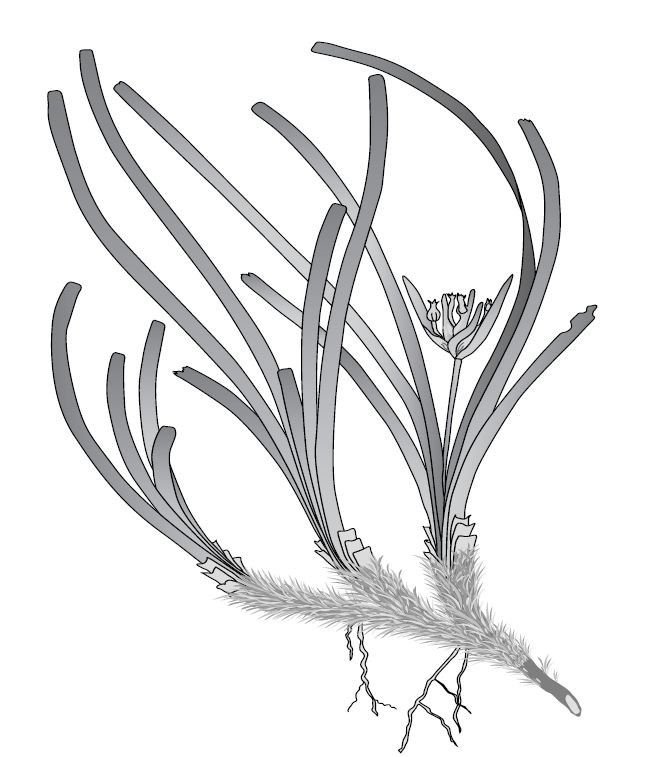
\includegraphics[scale=0.15]{Fig-1-6.jpg}
\caption{\textit{P.oceanica}.\\
Source \cite{Luque04}\label{Luque04}}
\label{fig:6}
\end{wrapfigure}

P.oceanica, making it highly recognizable and distinguishable from other seagrasses (Fig.\ref{fig:6}): having
usual length of 20-40 cm, in some cases they can reach up to 1 m \cite{Borum04}\label{Borum04}  (Fig.\ref{fig:8}).
Growing P.oceanica make a meadows which, in turn, consisnt of smaller patches, called “matte”
(Fig.\ref{fig:7}), a monumental construction made by the growth of rhizomes and leaves with entangled roots
and entrapped sediment \cite{Francour06}\label{Francour06}.
Representing one of the most productive Mediterranean ecosystems, \textit{P.oceanica} usually serves as a
perfect biological indicator for the assessment of the quality of waters and environmental health
\cite{Boudouresque89}\label{Boudouresque89}. Some authors \cite{Guidetti08,Montefalcone09}\label{Guidetti08} \label{Montefalcone09} used status and population dynamics of \textit{P.oceanica} as indicators for the evaluation

\begin{wrapfigure}{r}{0.4\textwidth}
\centering
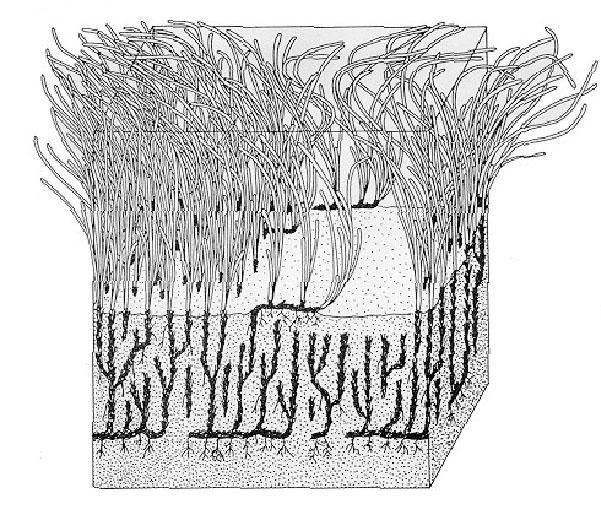
\includegraphics[scale=0.15]{Fig-1-7.jpg}
\caption{Scheme of matte structure of
P.Oceanica.\\ Source \cite{Pergent90}\label{Pergent90}}
\label{fig:7}
\end{wrapfigure}

of the meadow health status. \\
There are several environmental factors, determinating the growth of the \textit{P.oceanica}. The adaptation
to dry-summer subtropical climate reduces its extention to Mediterranean area only (Fig.\ref{fig:5}).
Besides, the distribution of the seagrasses changes with water depth: it is noticed \cite{Dural10}\label{Dural10} that
the highest flowering density is usually in the 4-7 m depth. 
\textit{P.oceanica} flowers appeared in shallow
stands in September while in November only in stands deeper than 15 m. This time delay is caused by
the different maximum summer temperatures at those depths \cite{Buia91}\label{Buia91}.

\begin{wrapfigure}{r}{0.4\textwidth}
\centering
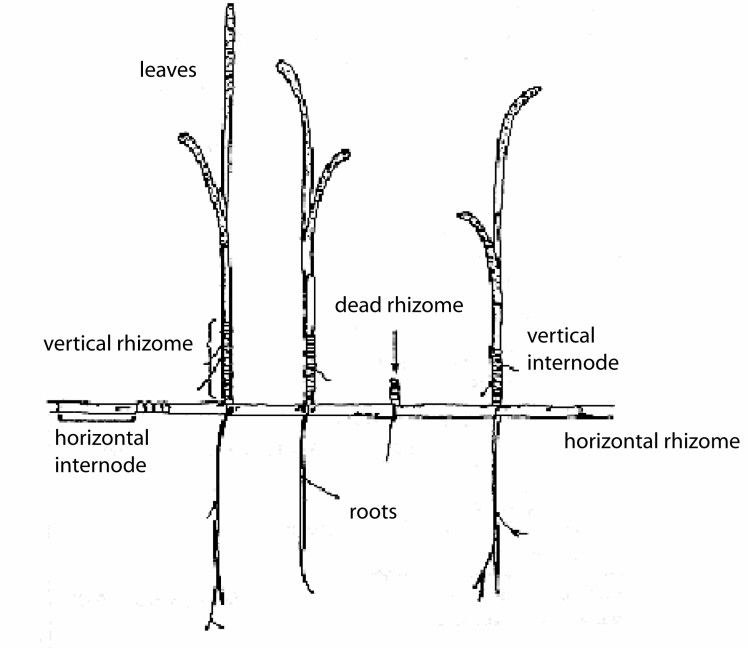
\includegraphics[scale=0.15]{Fig-1-8.jpg}
\caption{Structure and components of
P.oceanica \\ Source \cite{DiCarlo04}\label{DiCarlo04}}
\label{fig:8}
\end{wrapfigure}

The phenology of \textit{P.oceanica} is also affected by the coastal bathymetry: in the isolated meadows in
shallow waters plants have shorter and falciform leaves, compared to ones in the deeper and central
areas \cite{Dural10}\label{Dural10}. In \textit{P.oceanica} flower abundance is related to the structure of the meadow with
the maximal flower density in the densest stands, while the occurrence of flowering is regulated by
environmental factors \cite{Buia91}\label{Buia91}. Phenology of the \textit{P.oceanica} undergo
modifications with varying seasons during the year: during the flowering period (ca 3 months long)
the number of leaves on the flowering shoots decrease. Changes of the leaf growth also appear in the
flowering shoots with longer oldest leaves and shorter and narrower leaves induced during the
flowering \cite{Gobert01}\label{Gobert01}.

\subsection{Research problem}
Monitoring of the marine benthic ecosystems of seagrasses is essential for the environmental
assessment of the coastal zones. It increases our knowledge of the seagrass ecology, highlightes
threats to the seagrass and preventing them from possible losses and degrading and improves
techniques and methods of the underwater-based observations. Mapping the seagrass contributes to
the evaluating of the seagrass current distribution, analysis of its dynamics and changes over time, as
well as estimations of the degrading of seagrass meadows for the purpose of the coastal management.\\
Precise, correct and up-to-date information about the distribution of \textit{P.oceanica} is necessary for the
sustainable conservation of the marine environment and ecosystems in Mediterranean area, being an
important contribution to the environmental coastal zone management \cite{Pergent-Martini06}\label{Pergent-Martini06}.
However, mapping the sesgrass has limitations due to the specific location and characteristics of the
research object. The remote sensing techniques have traditionally been widely used for the seagrass
monitoring. 

\begin{wrapfigure}{r}{0.4\textwidth}
\centering
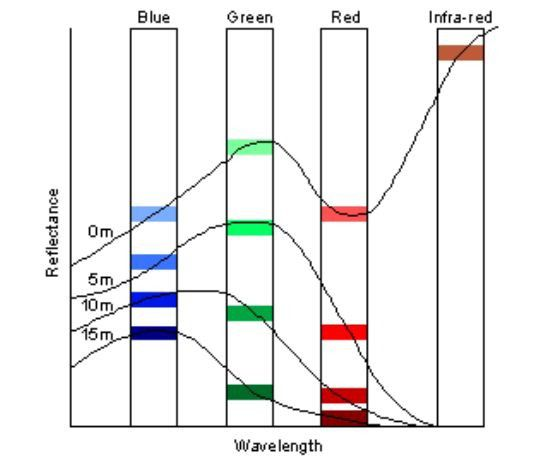
\includegraphics[scale=0.25]{Fig-1-9.jpg}
\caption{Spectra of the seagrass on different
depths (0 - 15 m). Source \cite{Edwards00}\label{Edwards00}}
\label{fig:9}
\end{wrapfigure}

The general overview of the application of various remote sensing data types (colour,
infrared, and black and white images) for the seagrass monitoring shows its high suitability and
potential as a research method \cite{Pasqualini01,Matarrese06}\label{Pasqualini01}\label{Matarrese06}. The using of the aerial
photographs as base maps for the seagrass meadows mapping is, perhaps, the most traditional
application \cite{McKenzie03,Kendrick00,Pasqualini99}\label{McKenzie03} \label{Kendrick00} \label{Pasqualini99}. The results of the image
processing of colour aerial photographs for the monitoring of littoral environment with seagrass beds
have been reported by several authors \cite{Kelly80,Walker89,Green96}\label{Kelly80} \label{Walker89} \label{Green96}.
Satellite imagery processing has also being used for the seagrass monitoring, due to their accuracy,
repeatability and informativeness as a source of data \cite{Dekker05b}\label{Dekker05b}, enabling regular temporal
coverage over the large remote areas and providing a cost-effective approach for the mapping of the
remotely located feature, such as underwater vegetation \cite{Jensen95}\label{Jensen95}. Satellite images provide
with detailed information on seagrass canopy and other environmental indicators \cite{Fyfe03}\label{Fyfe03}.
Various research papers report successful application of the image processing for the
seagrass mapping \cite{Calvo03,Dekker05a,Fornes06,Green96,Jackson07,Jensen95,Kendrick00,Lyzenga81,Malthus03,Matarrese08,Mount03,Pasqualini01,Pasqualini99,Pasqualini98a,Pergent-Martini06,Ralph05,Ribed02,Short01,Walker89}\label{Calvo03}\label{Dekker05a}\label{Fornes06}\label{Green96}\label{Jackson07}\label{Jensen95}\label{Kendrick00} \label{Lyzenga81}\label{Malthus03}\label{Matarrese08}\label{Mount03}\label{Pasqualini01}\label{Pasqualini99}\label{Pasqualini98a}\label{Pergent-Martini06}\label{Ralph05}\label{Ribed02}\label{Short01}\label{Walker89}. The application of the remote sensing data towards seagrass mapping is based on the spectral reflectance
 characteristics of the \textit{P.oceanica} seagrass, which enable its spectral discrimination from spectra of other seafloor types. 
It is proved \cite{Thorhaug07} \label{Thorhaug07} that the spectral signatures of different species of tropical seagrasses are well
distinguishable from each other. The application of the methods of images classification for seagrass
mapping is based on the classifying the pixels on the image according to their spectral reflectance
values \cite{Fornes06} \label{Fornes06}, so that the seafloor can be divided into several types: sand, rock, P.
oceanica, other vegetation, etc.
Other example of monitoring of \textit{P.oceanica} using remote sensing techniques \cite{Calvo03}\label{Calvo03}
reports the application of the CZCS images towards the case study of the Italian coast and shows
successful results of the neural-based classification using Isodata method of supervised classification.
In case of \textit{P.oceanica} meadows aerial and satellite images are particularly suited for the surveying
shallow waters \cite{Pasqualini98b}\label{Pasqualini98b} enabling to distinguish seagrass formations and dynamics of
the temporal evolution of seagrass meadows over the research area \cite{Pasqualini01}\label{Pasqualini01}.
However, using space borne satellite imagery for the seagrass mapping has certain limitations, due to
the uncertainties of the spectral signature of the seagrass at higher depths  (Fig.\ref{fig:9}), as well as some
optical particularities, e.g. light refraction under water, unevenness of the water surface, depths, etc.
Some problems can also arise in the images interpretations, as quite different objects may have
similar spectral reflectance, e.g. seagrass, dark-coloured bottom patches (mud), macroalgae.
The in-situ fieldwork including underwater videographic measurements is an important part of the
seagrass monitoring, and has been successfully applied towards seagrass mapping \cite{Haag08}\label{Haag08}.
The underwater measurements are used to validate the results and to receive detailed, accurate and
precise data for the selected locations. The underwater measurements cannot be applied for the whole
research area, however it provides with detailed monitoring along the route of the boat. Therefore, in
the selected locations it becomes a useful tool for the assessment of the distribution, density and
coverage of the seagrass along the tracklog. Besides, the underwater observations using scuba diving
equipment have been conducted for the measurements of depths.

\subsection{Research objective}
The current MSc research aims to explore the environmental conditions and dynamics of the spatial
distribution of \textit{P.oceanica} seagrass meadows along the Cretan coast, based on the remote sensing and
GIS techniques, knowledge about the coastal environment in Crete and integration of various data
from the following sources:
i) spectra of P.oceanica, carbonatic sand, silt and other seafloor types
ii) satellite imagery: Landsat, ASTER, MODIS, MERIS
iii) aerial photos: Google Earth
iv) in-situ fieldwork data of underwater videographic measurements
v) vector GIS layers.
The research aims to explore the dynamics of the environmental changes of the P.oceanica meadows
over time (2000-2010), as well as the extent of the spatial distribution over the whole island. The
main research objective is monitoring the seagrass \textit{P.oceanica} along the coasts of Crete, in order to
analyse the environmental changes of the P.oceanica meadows over the last 10 years (2000-2010)
and the spatial extent of its current distribution.
This research is supported by the in-situ measurements in two selected locations of the northern coast
of Crete (Ligaria beach in Agia Pelagia district and Xerocampos), using following methods of the
remote sensing techniques: underwater videometric measurements made by Olympus camera, aerial
Google Earth and satellite images from different sources, spatial GIS and statistical analysis.

\subsubsection{General objective}
The main objective of this study is to investigate the distribution of seagrass along the northern coast
of Crete using remote sensing techniques.
General objectives:
1) Mapping the spatial distribution of the seagrass \textit{P.oceanica} along the northern coasts of
Crete Island
2) Monitoring the dynamics of the environmental changes of the P.oceanica meadows over
time (2000-2010) in Ligaria beach, Agia Pelagia district.

\subsubsection{Specific objectives}
1. To apply remote sensing data (Google Earth aerial images, Landsat, SPOT satellie images)
for the monitoring of the seagrass meadows distribution
2. To study narrow-band spectral reflectance propoerties of \textit{P.oceanica} and other seafloor
cover types (sand and silt) using WASI swater colour simulation software
3. To use methods of the in situ diving observations and underwater videometric measurements
by Olympus camera in order to receive large-scale imagery of the P.oceanica mattes
4. To perform images classification (supervised and unsupervised) for the thematic mapping of
the P.oceanica seagrass distribution along the coasts of northern Crete.

\subsection{Research questions}
1. Is \textit{P.oceanica} spectrally distinct from other seafloor cover types with varying in-situ
conditions ?
2. Whether broadband and hyperspectral remote sensing data can be used for the mapping of
\textit{P.oceanica} ?

\subsection{Hypotheses testing}
A statistical testing will be used to compare between the spectral responses of the different seagrass
types, whether it is spectrally distinct and at least one pair is statistically different at every spectral
band.
Hypothesis Ho: seagrass types are not spectrally distinct from other seafloor types with
varying in-situ conditions, which means
Ho: μ1 =μ2 =μ3=...= μn.
The alternative Hypothesis Ha claims the opposite statement: seagrass is spectrally
distinct with varying in-situ conditions, Ho: μ$\neq$μ2$\neq$μ3$\neq$ ... $\neq$μn.
The distribution of the spectral responses at every spectral band is assumed to be normal as well as
the equality of the statistical variances.
The hypothesis testing is suggested to be carried out using the anova statistical test. The purpose of
anova test is to visualize in an effective and quick way the spectral differences between seagrass
species and their spatial distribution. Thus, the key hypotheses of the research will be tested to prove
whether the results of the research are accurate, reasonable and correct.

\subsection{Research scheme}

\subsection{Research approach}
Seagrass consistent monitoring and mappint is necessary and important for the sustainable coastal
development and conservation measures. Earlier, many seagrass meadows have been destroyed by
human activities in the coastal zone, mainly due to the ignorance of their existence, because
information on the seagrass bed exact location was not available \cite{Choo06}\label{Choo06}. Well-time seagrass
observations and mapping enables precise control of its spatial distribution, detection of any changes
in the seagrass landscapes, highlightes potential environmental threats in the coastal zone (e.g.
declining of meadows) before they become unmanageable for the coastal management services.
Choosing the right and most effective approach method for the seagrass monitoring is essential.
Remote sensing methods alone, though having evident advantages, are insufficient, because satellite
images of underwater habitats are notoriously difficult to identify and interpret. The best research
method should be based on the integrated approach, well described in various scientific works \cite{Brown02,Montefalcone06,Kirkman96}\label{Brown02} \label{Montefalcone06} \label{Kirkman96}, which includes combination of various
techniques of the seagrass monitoring, i.e. remote sensing imagery classification of aerial and satellite
images, GIS-based spatial analysis and ground in-situ surveys.
The current study is based on the application of the remote sensing data, broadband satellite imagery,
aerial images and the results of the underwater videographic measurements towards seagrass
mapping. Image classification is based on the principle of the differentiation between the spectral
signatures of various seafloor cover types. The spectrum of light coming up from the ocean surface in
shallow waters keeps information on the optical properties of the seawater components and benthic
substrate which can be read from their spectral signatures \cite{Werdell03}\label{Werdell03}. Spectral
reflectances, distinct for each seafloor cover type, enable their discrimination on the image. The preprocessing
of the images includes imagery corrections for atmospheric noises and effects of the water
column. Reflectance spectra of the seagrass canopy at different depths of the water-column are
analysed for the discrimination of their spectral signatures, enabling to separate various seafloor types
during classification. The results of the of imagery classification are analysed for the detection of the
dynamics in \textit{P.oceanica} seagrass distribution along the northern coasts of Crete. Aerial imagery from
Google Earth with high spatial resolution, suitable for the large-scale detailed mapping of seagrass
mattes, is used for the improvement of the accuracy of large seagrass meadows and separate mattes
within the meadows. The in situ underwater videometric measurements of the seafloor are collected
during the fieldwork in Crete, for the validation of the classification results and to determine the exact
current distribution of the \textit{P.oceanica} meadows. The image processing includes steps of the remote
sensing techniques, i.e. calibration, masking from land and cloud, atmospheric correction, sea surface
glint and depth effects correction as recommended \cite{Matarrese08}\label{Matarrese08}. During the image classification
working step the training sites for the supervised classification methods are designed, as well as its
control and trials of different classification approaches (Unsupervised, K-means or Isodata;
Supervised, Maximum Likelihood).
\pagebreak

\section[Overview of literature]{Seagrass monitoring: overview of literature and research resources}
%\markright{II. Seagrass monitoring: overview of literature and research resources}
%\renewcommand{\headrulewidth}{0.4pt}

\subsection{Seagrass global monitoring: history and perspectives}
Mapping and monitoring the seagrass is important for the environmental assessment of the marine
ecosystemsn in coastal areas. Regular tracking of current distribution of seagrass meadows, based on
correct information and cartographic visualization of seagrasses, is a preventive environmental
management, which helps to analyse potential environmental risks of coastal areas, decrease of the
number of species, loss of meadows and patches of the seagrasses.
The tradition of global seagrass mapping though has not a very long history comparing to the
terrestrial cartography, due to the technical difficulties of underwater observations, yet nowadays is
has become a successful, rapidly developping, increasingly popular and challenging research branch.
Seagrasses can be mapped using various approaches, with the most popular method of the remote
sensing application, enabling to detect and discriminate the substratum and various vegetation types
growing on the seafloor.
Several global seagrass surveys organise and provide regular monitoring of the segrass distribution,
health and species sustainability, amongst which the most world-known are, perhaps, the following
ones: \href{http://www.seagrassnet.org/}{Global Seagrass Monitoring project}, \href{http://www.seagrasswatch.org/}{Seagrasswatch}, 
located in Australia, \href{http://mediterranean.seagrassonline.org/}{the Mediterranean association Seagrass-2000},
\href{http://www.imedea.uib.es/index.php}{the Mediterranean Institute for Advanced Studies},
\href{http://www2.fiu.edu/~seagrass/}{Seagrass Ecosystems Research Laboratory in South Florida},
\href{http://www.flseagrass.org/}{Florida Seagrass organisation}, \href{http://www.seagrasses.org/}{the Seagrasses.org} and the 
\href{http://wsa.seagrassonline.org/}{World Seagrass Association}.
 These organizations aim at global seagrass monitoring, providing with
research results and reporting guidelines and manuals with standartized methods and
recommendations, specific for the seagrass research and monitoring. There are also university marine
centres and research institutes conducting seagrass monitoring and as a particular part of their
research. Their reports and guidelines were used for references in the current research.
Regular obserbvations and monitoring of the seagrasses are known since 1960s, mainly in tropical
regions (Australia). Since that time traditional methods of the seagrass monitoring and common
recommendations are being elaborated. The development of the underwater SCUBA diving
equipment and devices enabled to conduct underwater detailed measurements and observations
largely contributed to the improvement of the traditional in-situ observations of seagrass. From the
other side, development of the remote sensing methods and data acquisition from space contributed to
the new methods of seagrass mapping, using distance approach and generally based on images
classification.

\subsection{\textit{In-situ} observations of the seagrass meadows}
The traditional methods of in-situ seagrass monitoring include in general the following standard
scheme \cite{McKenzieetal03} \label{McKenzieetal03}. The seagrass is being sampled on the selected sites using transect lines,
quadrant frame, single point markers, markers, GPS and other equipment. The seagrass sampling is
taken on the regular way with observation polints covering the study area with normal distribution.
During the measurement process, the vertical photograph of the measurements frame is taken, and the
following points are traditionally estimated: percentage of the seagrass cover withing the quadrate,
species composition, sediment composition, canopy height, epyphyte abundance, algae percent cover,
count of microfauna and a specimen of seagrass is being taken. This scheme, well described by
McKenzie \cite{McKenzieetal03}\label{McKenzieetal03} is widely used and well-known among the marine biologists and
seagrass researchers. Applications of the in-situ seagrass observations of the structuring epiphyte
community composition in the P.oceanica ecosystems in Mediterranean Sea is, for example,
described by Villegas \cite{Villegas06}\label{Villegas06}. Realization of traditional methods for mapping seagrass usually
involves intensive and time-consuming in-situ observations during the fieldwork, as, for example,
reported by Iverson and Bittaker \cite{Iverson86}\label{Iverson86}. Other methods of seagrass in-situ monitoring are based on
using the active hydroacoustic sonar sensors that send towards a sea floor a signal of energy and then
collect the return echoes for the analysis, yet this requires specialised equipment and is mostly used in
the depth waters, combined with bathymetric measurements. Another limitation of the acoustic
techniques is that they are not effective at identifying the composition or even the presence of
submerged aquatic vegetation such as seagrasses and seaweeds \cite{Werdell03}\label{Werdell03}, because
initially acoustic methods were intended for the bathymetric surveying, i.e. they are not adjusted for
the benthic habitat discrimination. The results of the in-situ measurements and observation are usually
managed and treated using integrated GIS approach, as, for example, reported by Schmieder \cite{Schmieder97}\label{Schmieder97}.

\subsection[Measuring water optical properties]{Measuring water optical properties: \\hyperspectral radiometers}
The application of the remote sensing data for seagrass mapping is based on our knowledge of the
spectral reflectance properties of the target objects, and using it for the classification of these objects
on the image. In case of seagrasses it is spectral reflectance of the seafloor cover types, which can be
analysed using measurements of optical properties of sea water: radiance and irradiance.
Optical remote sensing methods can get through the clear waters to approximately 15–30 m \cite{Mumby04}\label{Mumby04}.
 When sunlight enters the waters and goes down into the water column, parts of the
electromagnetic energy are absorbed and scattered, which is determined by the optical and physical
properties of the water, e.g. concentration of suspended particles, chlorofill, coloured dissolved
organic matter (gelbstoff) that make up the water content \cite{Ackleson2003}\label{Ackleson, 2003}. Besides, light is strongly
dependent on wavelengths, i.e. it is greater in blue wavelengths (400 nm) than in others.

\begin{figure}
	\centering
	\subfloat [RAMSES-ACC-UV - Hyperspectral UVA/UVB Irradiance Sensor: 280-500 nm]{\label{fig:1-1a}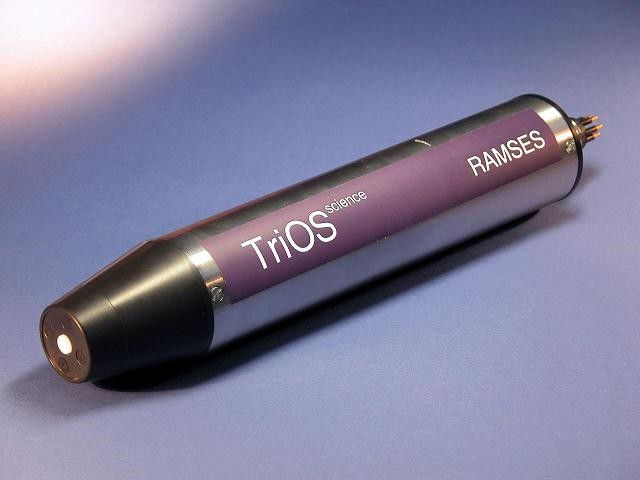
\includegraphics[width=0.4\textwidth]{Fig-2-1.jpg}}
	\subfloat [RAMSES-ARC - Hyperspectral UV-VIS Radiance Sensor: 320-950 nm.]{\label{fig:1-1b}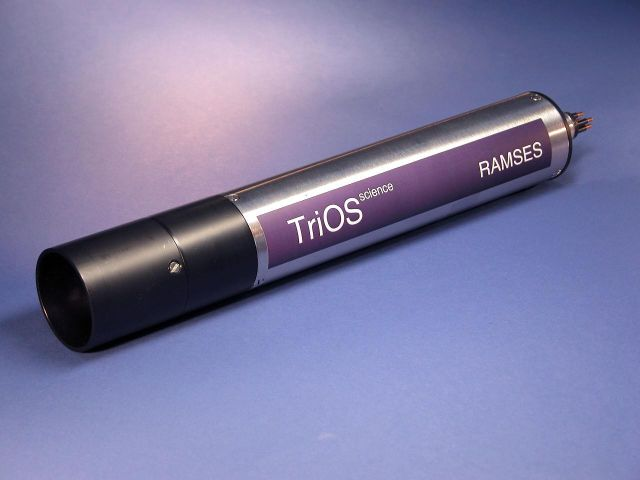
\includegraphics[width=0.4\textwidth]{Fig-2-2.jpg}}
	\caption{RAMSES Hyperspectral Sensors. Source: \href{http://www.trios.de}{Trios}}
	\label{fig:10}
\end{figure}

The optical properties of the sea water vary with different environmental conditions and reflect
current chemical content and physical specifics of the water, revealing the variability and distribution
of color of the sea waters, determined by the material in the water, e.g. chlorophyll, as well as its
physical properties, e.g. water absorption, attenuation, backscattering \cite{Maffione01a}\label{Maffione01a}.
Shallow waters generally contain more dissolved substances and suspended particles, which directly
influnces the transparency and colour of the waters of shelf zones \cite{Jerlov52}\label{Jerlov52}. Being highly
dynamic environments, coastal waters experience a variety of processes which alter their optical
properties incessantly. The effects of these processes influence application of the hyperspectral
remote sensing and reinforce other proceses \cite{Maffione01b}\label{Maffione01b}. Thus, waves and tides, increase
sedimentation processes which in turn may change microrelief properties and topology. 
The optical properties of the water are best reflected in the values of its radiance and irradiance,
which can be converted into spectral reflectance, or reflectivity. The spectral irradiance (E) is a
radiant flux of the electromagnetic solar radiation energy, received per surface unit area in a given
time (W·m−2·nm−1), while radiance (L) characterizes total emission or reflection that passes through
or is emitted from a particular area (W·sr−1·m−2 ·nm−1). Therefore, the spectral reflectance, or the
reflectivity of the object, can be estimated by the direct mathematical division of these first two
characteristics, and is expressed in persentage.
Therefore, the irradiance and radiance of the water should be measured in order to estimate spectral
reflectance of the various seafloor cover types. The optical measurements of the irradiance and
radiance of the sea water and bottom cover types of the seafloor can be received by the means of the
optical sensors spectroradiometers. There are several companies producing radiometers with various
characteristics and adjusted for defferent purposes, e.g. portable and miniature spectrometers from
\href{http://www.stellarnet.us}{StellarNet}, Hyperspectral Ocean Colour Radiometer (HyperOCR) sensor by
\href{http://www.satlantic.com}{Satlantic}, traceable spectroradiometers by \href{http://www.orboptronix.com}{Orbotronix} 
and lots of others. Among other radiometers there are ones designed by the \href{http://www.trios.de/}{Trios company} producing
optical sensors, GER-Series Field portable spectroradiometers from
\href{http://www.spectrapartners.nl/}{SpectraPartners}, etc. Trios-RAMSES hyperspectral radiometers
(Trios-RAMSES Hyperspectral UVA/UVB Irradiance Sensor and RAMSES-ARC Hyperspectral UV-
VIS Radiance Sensor) are small-sized, low power-consumpting, flexible for fieldwork yet with high
level of precision, specially calibrated for air and for water application as well as colour
measurements  (Fig.\ref{fig:10}). These products have been used for the radiance and irradiance
measurements in Agia Pelagia bay, Crete island, 2009.

\subsection[Application of remote sensing data]{Application of remote sensing data towards seagrass mapping}
Various methods and approaches have been applied towards mapping of the seagrasses, based on
digitized aerial photographs, GPS data, remote sensing and SCUBA-based fieldwork measurements.
SCUBA-based in-situ observations, though providing high resolution and accuracy results in seagrass
mapping, is limited in application, because of their time consumption, weather-dependancy and
unsuitability for the case of monitoring large areas of water for small-scale mapping. Methods of
underwater videography with GPS is a tool of seagrass monitoring which has certain advantages, i.e.
high spatial and visual resolution, non-destructive sampling, effectiveness at all depths and rapid data
collection in the field \cite{Schultz08}\label{Schultz08}. However, it cannot cover large areas for small-scale mapping.
Remote sensing techniques offer clear advantages over other methods of in-situ field measurements
and seagrass observations, mentioned above. Preference of the remote sensing methods consists in
their weather-independency, cost-effectiveness, accuracy and spatial coverage, which enables
periodic monitoring of the seagrass mewdoes and gives access to the distant and unapproachable
areas. Integrated together with GIS vector layers and maps, remote sensing data enable historical
mapping \cite{Carter08,Ardizzone06}\label{Carter08} \label{Ardizzone06} and assessment of change detection.\\
However, application of the remote sensing techniques for mapping of submerged vegetation,
seafloor cover types and benthic vegetation, inter alia seagrasses, are still in their development.

\begin{wrapfigure}{r}{0.4\textwidth}
\centering
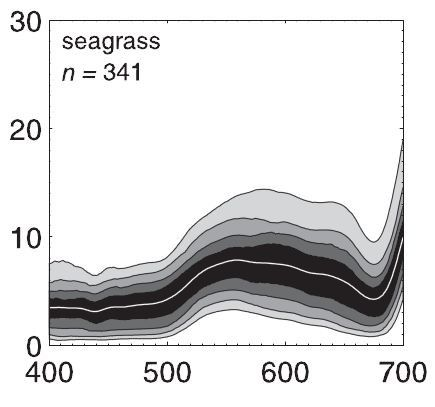
\includegraphics[scale=0.30]{Fig-11.jpg}
\caption{In situ optical reflectance spectra of
seagrass. Shaded areas - percent of spectra lying within
the range of reflectance. White lines - mean spectra.
Source: \cite{Hochberg03b}\label{Hochberg03b}}
\label{fig:11}
\end{wrapfigure}

Approaches and methods for seagrass protection and monitoring still remain location specific or, at
least, nation specific, depending to large extent on the tools available for researchers \cite{Mellors09a} \label{Mellors09a}.
Universal, international, standardised methods for seagrass directly for seagrasses
as such still should be developed. Various case studies have been performed, yet their mostly report
methods adjusted for particular areas, without evaluating starndard general algorithms that could be
extrapolated towards other regions. \\ Application of the remote sensing towards seagrass mapping is
generally based on the assumption that various types of the seafloor bottom have different
characteristics of the reflectivity, which is visually expressed in distinct colors of the objects. In its
turn, reflectivity of the sediments is affected by the water optical properties and content. For
example, Stephens \cite{Stephens03}\label{Stephens03} prove that microalgal biomass and community structure affect
hyperspectral reflectance of sediments, which enable to estimate total microalgal biomass from
measurements of hyperspectral reflectance. Spectral measurements of the target objects are made
my the means of the radiometers, which receive and register the amounts of enegry (radiance and
irradiance) from the objects. \\ Measuring optical properties of water allow to calculate spectra of the
objects and to discriminate them on the aerial and satellite images. Thus, various scientists report
success in spectral discrimination of submerged vegetation and other seafloor cover types on imagery
using hyperspectral optical properties of the sea water for the assessment of benthic habitats \cite{Lewis01,Louchard03,Dehouck08,Werdell03}\label{Lewis01} \label{Louchard03} \label{Dehouck08} \label{Werdell03}.
Studies of spectral reflectances of the different seagrass species comparing to the spectra of sand and
other seafloor cover types \cite{Vahtmae06}\label{Vahtmae06} prove that spectra of green, brown and red benthic
macroalgae differ from each other, as well as from sand and deep water reflectance spectra. These
differences are well detectable by the means of the remote sensing research methods. Comparing to
the terrestrial plants, aquatic vegtation inter alia seagrass cannot be detected using red edge of the
spectrum, as these wavelengths are significantly absorbed by water \cite{Kirk94}\label{Kirk94}, as well as by
scattering and absorption by phytoplankton. Some authors \cite{Dierssen03}\label{Dierssen03} also use
spectrally based radiative transfer approach to quantitatively estimate shallow-water bathymetry and
leaf area index (LAI) of the seagrass. The spectral reflectances in general are the
result of the spectral absorption in different bands, typical for each target object.
Spectral reflectance of the seagrass  (Fig.\ref{fig:11}) is largely influenced by the water
depth where it is located, and is generally decreasing in values by increasing depths.
The most important spectral diapason for marine mapping of submerged vegetation
and, particularly, for seagrass, is 350-800 nm \cite{Barille09}\label{Barille09}.
Using airborne imagery for retrospective data (before 1970s) together with the most
recent imagery allows to detect changes in seagrass distribution on over different years
and to analyse dynamics of the seagrass distribution\cite{Ball09}\label{Ball09}. Another important advantage
of the application of the remote sensing data for mapping of submerged aquatic vegetation has
commertial nature: using remote sensing data and methods enables more low-cost and up-to-date
seagrass mapping \cite{Mumby99}\label{Mumby99}, and is especially useful for the areas where the fieldwork data
capturing is unavailable.

\begin{wrapfigure}{r}{0.5\textwidth}
\centering
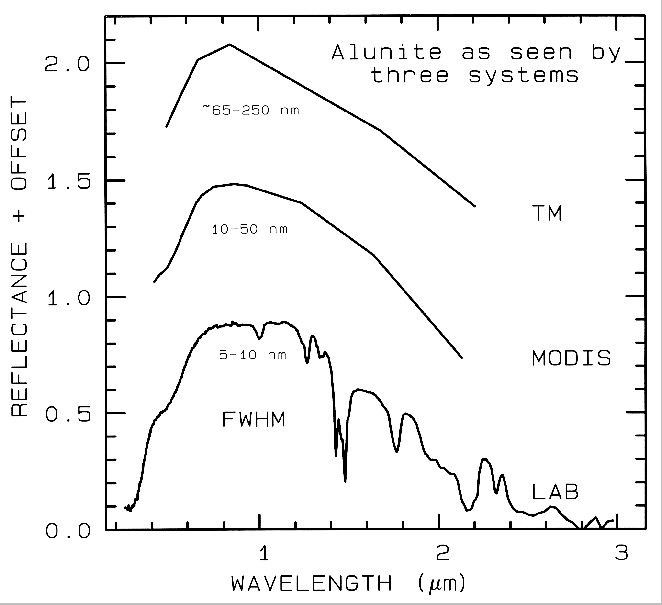
\includegraphics[scale=0.25]{Fig-12.jpg}
\caption{Difference between broaddand
multispectral and hyperspectral resolution of
spectral signatures. Source: \cite{Clark99}\label{Clark99}}
\label{fig:12}
\end{wrapfigure}

Seagrass meadows may reach spatial scales from several up to hundreds of metres, therefore they are
susceptible by the means of satellite imagery from remote sensors, both with moderate resolution
(e.g., \href{http://landsat.gsfc.nasa.gov/}{Landsat MSS, Landsat TM, Landsat ETM+}, \href{http://envisat.esa.int/instruments/meris/}{MERIS}, \href{http://asterweb.jpl.nasa.gov/}{ASTER}, \href{http://modis.gsfc.nasa.gov/}{MODIS}) and high resolution as
well (e.g., \href{http://www.satimagingcorp.com/gallery-ikonos.html}{IKONOS}, \href{http://www.digitalglobe.com/index.php/85/QuickBird}{Quickbird}, \href{http://www.spotimage.fr/}{SPOT}, \href{http://www.itres.com/products/imagers/casi550}{CASI}). The possibility of their application towards seagrass mapping
vary and is limited by the technical characteristics (Table \ref{tab:1}) and resolution of these sensors  (Fig.\ref{fig:12}). In the next subparagraphs
we briefly discuss the limitations and research experience of the using of various imagery
for the seagrass mapping.

\begin{table}[htbp]
\caption{\textbf{Characteristics of selected ocean-colour sensors}}
\begin{center}
\rowcolors{1}{OldLace}{FloralWhite}
\begin{tabular}{|p{2cm}|p{20mm}|p{15mm}|p{17mm}|p{15mm}|p{15mm}|p{15mm}|}
\hline\hline
\textbf{Satellite Sensor:} & {\textbf{Landsat}} & {\textbf{SPOT}} & {\textbf{ENVISAT}} & {\textbf{Terra}} & {\textbf{GeoEye}} & {\textbf{Nimbus 7}} \\ \hline\hline
	\textbf{Origin} & USA & France & Europe (ESA) & USA (NASA) & USA & USA \\ \hline
	\textbf{Instrument} & \textit{TM, ETM+} & \textit{Pan, XS} & \textit{MERIS} & \textit{MODIS} & \textit{SeaWiFS} & \textit{CZCS}\\ \hline
	\textbf{Number of channels} & 8 & 6 & 15 & 36 & 8 & 5 \\ \hline
	\textbf{Wavelength coverage} & 185-1700 & 500-1750 & 412.5- 900 & 469-1640 & 412-865 & 443-750 \\ \hline
	\textbf{Ground resolution (nadir), m} & 15-pan,30(MS),60 (TIR) & 2.5, 5, 10,20 & 1.2 km/300 m & 1.0 km & 1.13 km & 825 m \\ \hline
	\textbf{Band Width (nm)} & 0.45-10.4 & 10,20 & 2.5,7.5,9,10 14,20 & 0.18,0.3,0.5,10 - 50 & 20,40 & 20,100 \\ \hline
	\textbf{Launched} & 1972, 1999 & 1986 & 2002 & 1999 & 1997 & 1978 \\ \hline
	\textbf{Recurrent period, days} & 16 & 24 & 35 & 16 & 16 & 16 \\ \hline
\end{tabular}
\end{center}
\label{tab:1}
\end{table}



\subsubsection{Review of multispectral imagery used for seagrass mapping}
Seagrass mapping using remotely sensed data from multispectral sensors is based on the classification
and discrimination of the seafloor types using their spectral characteristics in different wavebands.
Perhaps, the most known imagery, widely used in the remote sensing mapping, is received from the
group of Landsat sensors, known for its historical, pioneeer role in the satellite industry.
Being the longest running satellite system, lunched in 1972, Landsat is the only source of archival
data going back to 1984 at a sufficient spatial resolution \cite{Dekker05}\label{Dekker05}, which makes its data
desirable for historial mapping or environmental analysis of change detection of the seagrass
landscapes.
The Landsat TM and Landsat ETM+ data, with the most recent from sensor Landsat 7, an advanced
and multispectral scanning, launched in 1999, proved to be feasibile and useful for the mapping of
submerged vegetation, such as seagrasses or coral reefs. The successful applications of the imagery
Landsat TM towards the seagrass mapping, were reported in numerous research works \cite{Palandro03,Gullstroom06,Wabnitz08,Bierwirth93,Ferguson97,Rasib97}\label{Palandro03} \label{Gullstroom06} \label{Wabnitz08} \label{Bierwirth93} \label{Ferguson97} \label{Rasib97}. The Landsat data are particularly suitable for the
case of change detection of seagrass landscapes at a decadal scale, because being the main sensor
onboard the Landsat satellites, Landsat Thematic Mapper (TM) provides the longest time series
available for change detection analysis over submerged vegetation \cite{Palandro03}\label{Palandro03}.

\begin{wrapfigure}{r}{0.5\textwidth}
\centering
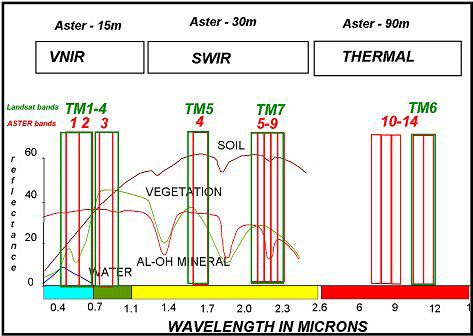
\includegraphics[scale=0.35]{Fig-13.jpg}
\caption{Band coverage of ASTER and Landsat channels on
the e/m spectrum. Source:\cite{Kalinowski04}\label{Kalinowski04}}
\label{fig:13}
\end{wrapfigure}

Another well-known multispectral sensor, SPOT provides multispectral imagery with a spatial
resolution of 10 m, covering covers a surface area of 3600 km² (60*60 km swath), 26-day
orbital repeat cycle for nadir viewing and imagery with a spatial resolution 20 - 2.5 m
\cite{SPOT}\label{SPOT}. \href{http://www.spotimage.fr/}{SPOT} imagery was used for mapping beds of Posidonia oceanica in the
Mediterranean Sea \cite{Pasqualini05} \label{Pasqualini05}. The \href{http://www.satimagingcorp.com/gallery-ikonos.html}{IKONOS}, offering multispectral and panchromatic imagery, was the first to collect publicly
available high-resolution imagery at 1- and 4-meter resolution from \href{http://www.geoeye.com}{Geoeye}. IKONOS
imagery has been applied for the seagrass mapping due to its high resolution and accessibility. Thus,
the results of image classification in case study of shallow-water marine environment \cite{Mumby02}\label{Mumby02}
made using IKONOS, Landsat TM, and CASI, show that in the blue part of the
spectrum, the best results are achieved by IKONOS and CASI, while Landsat TM has not high
enough resolution. It may be caused to some extent by the loss of the radiance contrast, atmospheric
Rayleigh scattering and defects of scattering. However, comparing between CASI and IKONOS, the
same authors prove that CASI enable to receive still more accurate results of the the classification
than IKONOS \cite{Mumby02}\label{Mumby02}.
Another comparative analysis of the application of \href{http://www.itres.com/products/imagers/casi550}{CASI}, Landsat and \href{http://www.digitalglobe.com/index.php/85/QuickBird}{Quickbird} imagery \cite{Phinn08}\label{Phinn08}
 demonstrates the high suitability of CASI images for the fine-scale mapping of seagrass
landscapes. Thus, CASI and Quickbird-2 images enable to identify even separate seagrass species
with small width and heterogeneous nature of the seagrass patches, which could not be detected using
Landsat TM images with their 30*30m resolution.
Advanced Spectrometer for Thermal Emission and Reflection Radiometer (\href{http://asterweb.jpl.nasa.gov/}{ASTER}), launched in
1999 onboard Terra sensor, provides high-resolution images of the Earth in 15 different bands of the
electromagnetic spectrum, ranging from visible to thermal infrared light  (Fig.\ref{fig:13}). It has diverse
subsystems for the visible near infrared (VNIR) with 15 m resolution, shortwave infrared (SWIR), and
thermal infrared (TIR) wavelength regions \cite{Kalinowski04}\label{Kalinowski04}. For each channel there is separate
onboard calibration (OBC) system, telescope with independent pointing and different detector technsology \cite{Arai05}\label{Arai05}. 
This makes ASTER imagery expecially suitable for the application towards detailed
mapping of surface temperature, emissivity and reflectance of objects and bathymetric elevations as
well. Successful application of the ASTER imagery towards mapping of submerged vegetation
reported, for example, by Hirose \cite{Hirose04} \label{Hirose04}. Other multispectra images have also been used for the
seagrass interpretation. For example, the success of using imagery from the multispectral airborne
scanner Daedalus AADS1268 is reported by Heege et al \cite{Heege03}\label{Heege03} where they aim at classification of
macrophytes in shallow waters of the Lake Constance.
In regard to the methods chosen for the image interpretation, the supervised classifications proves to
be the most worthy in a majority of case studies \cite{Palandro03,Peneva08}\label{Palandro03} \label{Peneva08}. While
often methods of the unsupervised classification are used as a tool for classifying submerged object
and features on the multispectral images and aerial imagery \cite{Fletcher09}\label{Fletcher09}, it still does not
provide common algorithms that can be applied to other images and regions. Thus, the strength of the
optical signal coming from the various types of the seafloor is strongly influenced by the effects of the
water column, its depth and chemical properties. Yet methods of the unsupervised classification
overleap mixed spectral effects of the water column which shift the real values of the spectra, with the
pure reflectance from the benthos; as a result, it may cause significant errors \cite{Dierssen03}\label{Dierssen03}.
 Therefore, for the accurate assessments of various seafloor cover types, water
column depth and its optical properties, methods of supervised classification should be preferably
used as being more suitable in classification and interpretations of imagery.
While this and other studies \cite{Phinn08}\label{Phinn08}demonstrated the advantages and success of the
application of multispectral imagery for the spectral discrimination of the seafloor cover types and
mapping the submerged landscapes on the basis of pixels classification, the application of data from
hyperspectral sensors has better potential due to their higher resolution.
\pagebreak

\subsubsection{Review of hyperspectral imagery used for seagrass mapping}
The application of the hyperspectral sensors is most effective and provide more accurate classification
results (Fig.2.1.), 

\begin{wrapfigure}{r}{0.5\textwidth}
\centering
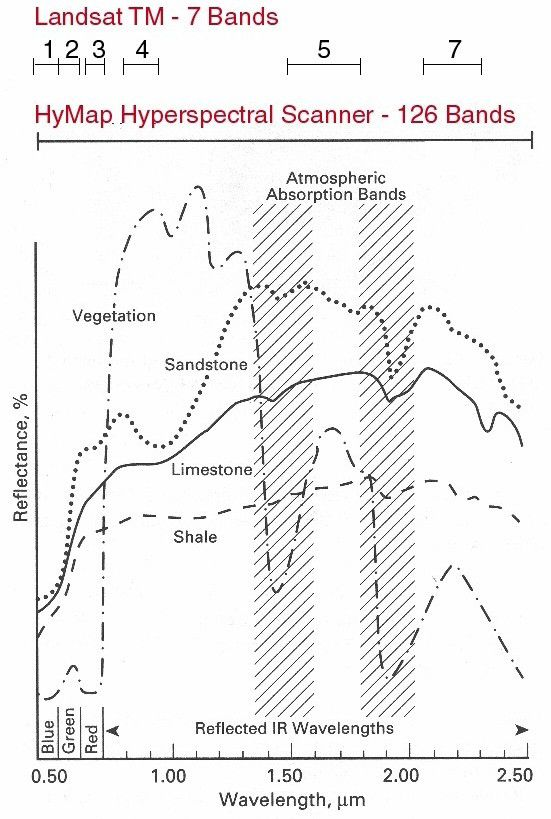
\includegraphics[scale=0.30]{Fig-14.jpg}
\caption{Multispectral vs. hyperspectral band
coverage. Source: \cite{Sabins97}\label{Sabins97}}
\label{fig:14}
\end{wrapfigure}

due to their higher spectral resolution \cite{Bharathi03}\label{Bharathi03} with interval
narrows to 10 nanometers, while broadband sensors are limited to the spectral width of ca
150 nm (Fig.\ref{fig:14}). 
Hyperspectral imagery is acquired through the simultaneous acquisition of images in many
narrow, contiguous spectral bands from hyperspectral scanners (mostly) cover the 400-
to 2500-nm spectral bands \cite{Schmidt03}\label{Schmidt03}.
Perhaps, the most advantageous and general characteristics of hyperspectral imagery is its
high spectral resolution, desirable for the case of seagrass monitoring. 

\begin{wrapfigure}{r}{0.5\textwidth}
\centering
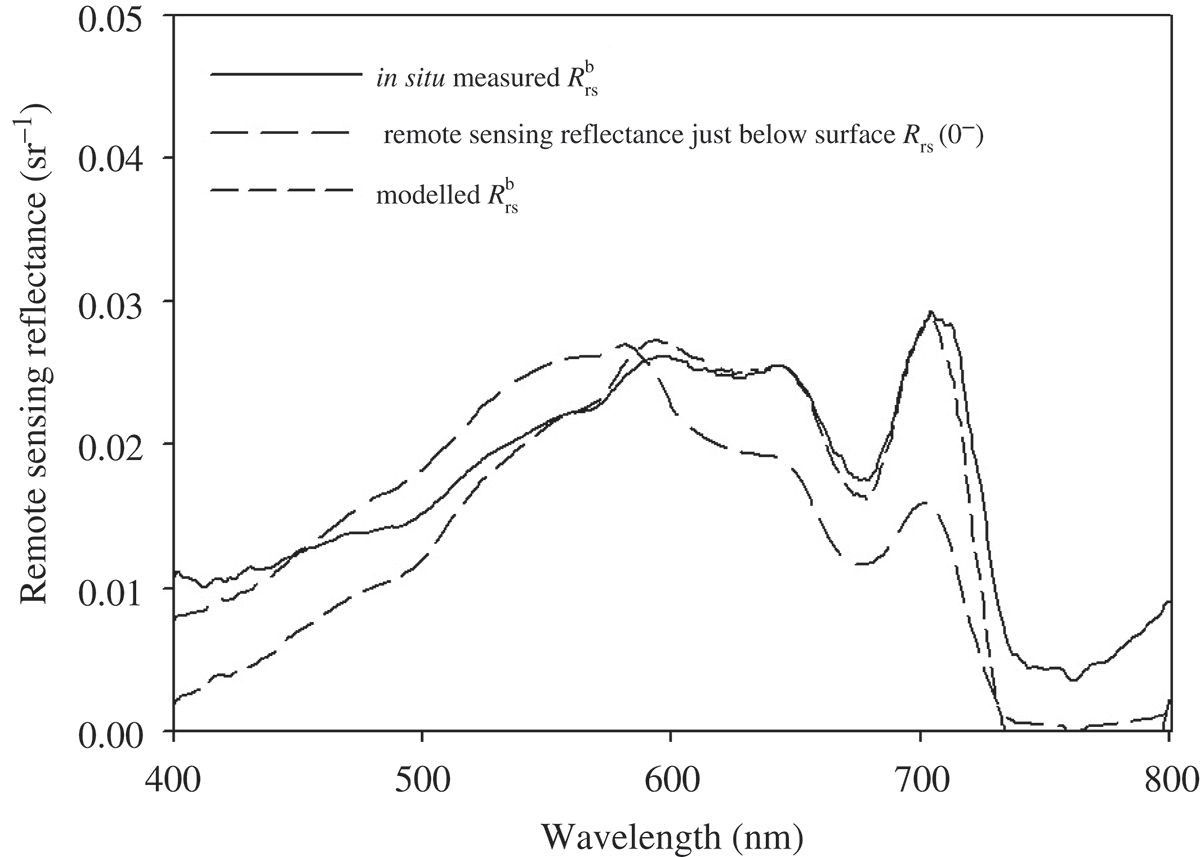
\includegraphics[scale=0.15]{Fig-15.jpg}
\caption{Reflectance spectra of seagrass; Rrs(0-)
- subsurface RS reflectance; Rrs b - the bottom
reflectance. Source:\cite{Yang10}\label{Yang10}}
\label{fig:15}
\end{wrapfigure}

The most suitable
scanner fit for detailed seagrass mapping would cover bands of 550-750 nm and have a spectrum
resolution of 5-15 nm \cite{Fyfe04}\label{Fyfe04}, which exactly characterizes typical airborne and
hyperspectral satellite scanners. Important features may be detected in the narrow
wavelengths of hyperspectral imagery, while this information can be lost in the broader
wavelengths of other sensors. With its 126 spectral bands, HyMap imagery enables to
distinguish features of interest, i.e. seagrass types \cite{Peneva07}\label{Peneva07}, which is the major
advantage of the of hyperspectral data for mapping landscapes of the seagrasses.
While comparing multispectral imagery with airborne hyperspectral, the last one showed higher
overall accuracies \cite{Phinn08}\label{Phinn08}. Several, regular and narrow (10 nm) spectral bands, specific for
hyperspectral imagery, are strong tool enabling to detect even slight and subtle differences in the
spectral reflectances between various seafloor types, e.g. different seagrass species at diverse depths,
algae, corals, dark-coloured sands or other types of sediments \cite{Hochberg03a}\label{Hochberg03a}. 
Therefore, there is great potential of the application of hyperspectral remote sensing imagery towards seagrass
mapping at species level, as long as they are distinguishable spectrally (Fig.\ref{fig:15}) which, for example, has been
tested in the case study of Australian marine ecosystems by Fyfe \cite{Fyfe04}\label{Fyfe04}. Application of various
classifications methods, inter alia maximum likelihood, minimum distance and means, towards
hyperspectral imagery \cite{Peneva08}\label{Peneva08}, combined with fieldwork measurements ensures accurate
mapping results with the maximum likelihood methos producing the best results.
Therefore, accurate mapping of the seagrass landscapes and other seafloor types using remote sensing
approaches requires application of high-spatial resolution (higher than 5 m) or hyperspectral imagery.
Comparative analysis of the application of hyperspectral and multispectral imagery towards the
seafloor types classification \cite{Hochberg03a}\label{Hochberg03a} demonstrates that coral, seagrasses and
sand wery vell distinguishable in their spectra with an overall classification accuracy of 98 percent.
However, the use of data from various sensors, both hyperspectral and multispectral, are possible and
reasonable, as soon as it meets the research specific objective. 
Thus, the use of multispectral imagery
with high spatial resolution is preferable to using hyperspectral medium resolution data in case of
mapping benthic vegetation in areas where the spatial heterogeneity is very high \cite{Vahtmae07}\label{Vahtmae07}.

\section{Materials and methods}
%\markright{III. Materials and methods}

The research is technically based on WASI, for the analysis of spectral signatures, \href{http://www.esri.com/software/arcgis/index.html}{ArcGIS} and \href{http://www.erdas.com/products/ERDASIMAGINE/ERDASIMAGINE/Details.aspx}{Erdas Imagine} software for the processing and analysing of aerial and broadband images, Google Earth and  \href{http://landsat.gsfc.nasa.gov/}{Landsat}.
\href{http://www.esri.com/software/arcgis/index.html}{ArcGIS 10.0} software is used for the spatial analysis, general mapping and cartographic layout
presentation; the raster processing techniques are applied for the detection of seagrass spatial
distribution using supervised classification.
The research data include Google Earth aerial images and scenes from the \href{http://landsat.gsfc.nasa.gov/}{Landsat TM and ETM+}
covering research period of 10 years in the same year time, taken from \href{http://www.usgs.gov/pubprod/}{USGS}, \href{http://glovis.usgs.gov/}{GloVis}, \href{http://www.osdpd.noaa.gov/ml/index.html}{NOAA} and \href{http://glcfapp.glcf.umd.edu:8080/esdi/index.jsp}{The Earth Science Data Interface}. 
The satellite imagery provides
vital information of the most recent changes in \textit{P.oceanica} within the coastal areas, as well as the
condition (poor or destroyed).
The raster processing includes making mosaic-like covering for the whole research area. The Google
Earth images are most appropriate for the detailed mapping than stellite than \href{http://landsat.gsfc.nasa.gov/}{Landsat} or \href{http://asterweb.jpl.nasa.gov/}{ASTER} enabling to produce accurate maps with correct results. Therefore, the main set of images for the
current work is Google Earth aerial images. The  \href{http://landsat.gsfc.nasa.gov/}{Landsat} images are used for the general overview.
Besides aerial and satellite photographs, data acquired during the fieldwork (21 Sep – 11 Oct) are
necessary addition to the mapping helping to solve problems of interpretation during the images
classification \cite{Pasqualini98a}\label{Pasqualini98a}. Therefore, this work includes sampling of the in-situ
measurements of the seagrass distribution.
The sampling stations were located in two candidate places on the northern (Ligaria) and southern
(Xerocampus) parts of Crete island, as these regions are well suitable for the seagrass, due to the
annual mean water temperatures and geological factors, i.e. seafloor conditions and sediments. The
field campaign has been carried out during the September-October period 2010. 
The information about the location of the seagrass (mostly represented by the P.oceanica species) is useful for the
understanding of the relationship between the spatial distribution of the seagrass and the environment
of the selected areas of Cretan beaches. The results of the videographic measurements are used for the
seafloor types detection, because the objects represented on the photos can be well distinguished and
classified according to the following well-known characteristics \cite{Butler87}\label{Butler87}: size (yet some
measurements are necessary for the similar-looking objects); shape (the general form is most reliable
evidence for identification); colour (common and reliable object indicator); texture (when changes in
tone are too small to be distinguishable, texture may assist identification, e.g., stippled, granular,
rough, smooth, etc.); associated features (those usually found near other objects, e.g., rocks and soil).

\pagebreak

\subsection{Study area}
General area: Island of Crete, Greece (Fig.\ref{fig:16}).\\
The study area of the current MSc research is located in the shallow areas of the Ligaria beach, Agia
Pelagia and Xerocampos, Crete island, Greece (Fig.\ref{fig:17}). These shelf areas have maximal depth of four meters.
Seagrass sampling has been performed at two stations at a depth of 4 meters, in the following selected
areas:
1. Ligaria beach (Agia Pelagia district), 36°20′N 22°59′E
2. Xerokampos, 35°12′N 26°18′E
3. Agia Pelagia, 36°20′N 22°59′E

\begin{figure}[h]
\centering
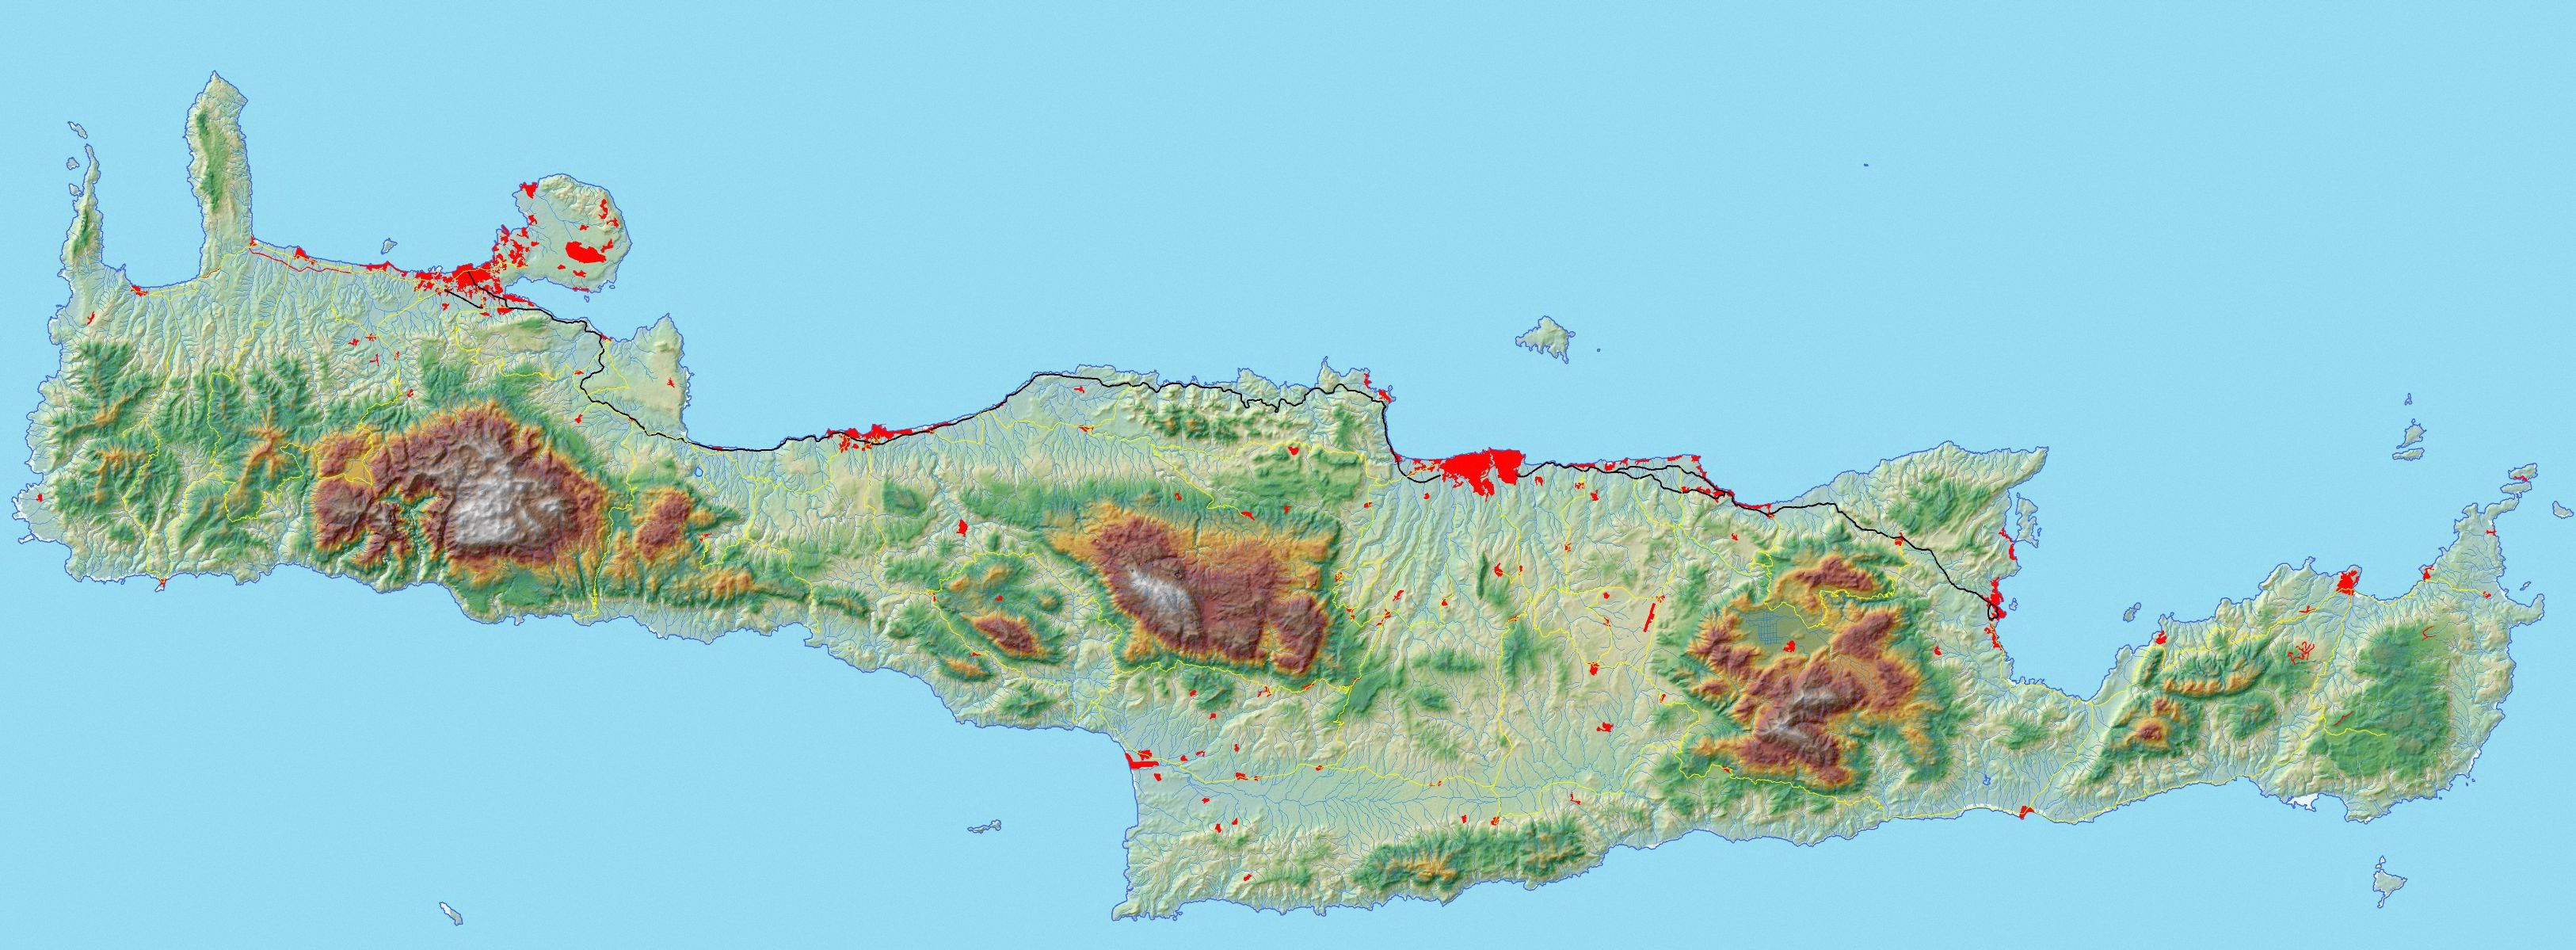
\includegraphics[scale=0.10]{Fig-16.jpg}
\caption{Study area: Crete island}
\label{fig:16}
\end{figure}

\subsection{Fieldwork data collection}
Seagrass sampling has been performed at two research stations at Crete island - Ligaria beach
(36°20′N 22°59′E) and Xerokampos (35°12′N 26°18′E), at depths lesser than 4 meters. 

\begin{figure}[h]
\centering
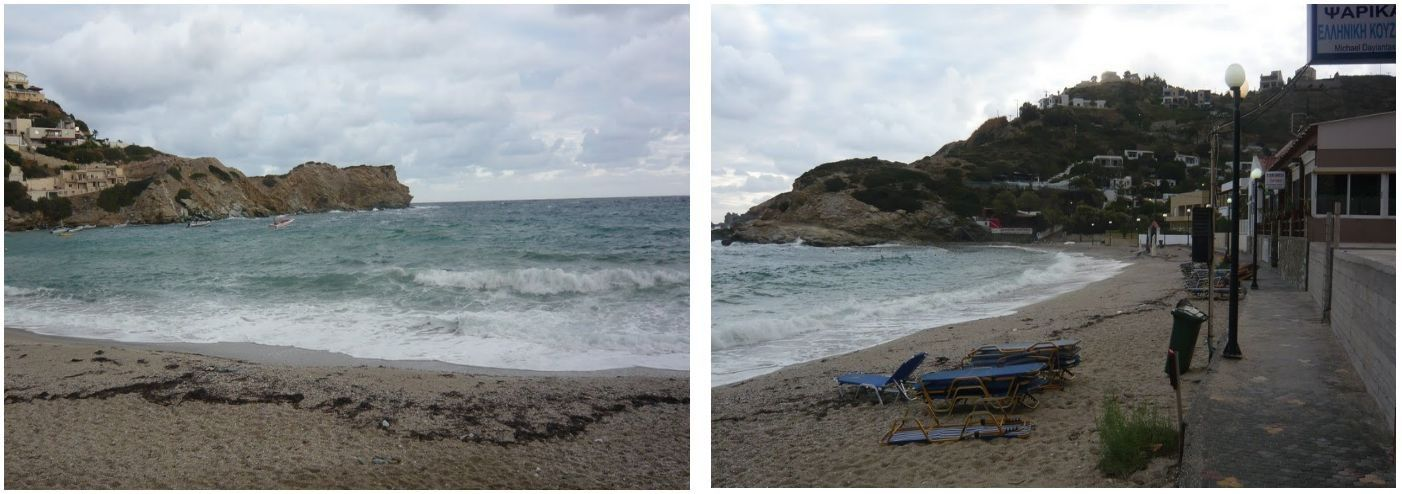
\includegraphics[scale=0.25]{Fig-17.jpg}
\caption{Study area: Ligaria beach, Crete island}
\label{fig:17}
\end{figure}

The Ligaria Beach is a narrow, sandy and pebble beach (Fig.12), located ca 15 km north-west from Heraklion.
The in-situ measurements were conducted during the fieldwork in the period 21.09.2010-11.10.2010.
The fieldwork on seagrass monitoring included visual estimations and photo- and video footage of the
above-ground seagrass patches, sediment seafloor cover types, species compositions, water depth and
geograpic locations recorded using GPS.

\subsubsection{Fieldwork equipment}
The research materials and equipment were provided by \href{http://www.nhmc.uoc.gr/index-2.htm}{the Natural History Museum of Crete}, the \href{http://www.uoc.gr/Department/index.html}{University of Crete} and the ITC, and included the following items (Fig.\ref{fig:18}): 1) three iPAQs; 2)
three GPS; 3) Three underwater video cameras, Olympus ST 8000, suitable for
photographing up to up to 33 foot depths and high-resolution 12.0-Mpixel image sensor; 4)
Markers and cords for the depths measurements; 5) Waterproof plasctic Otterbox for keeping the
iPAQ dry; 6) \href{http://www.padi.com/scuba/}{SCUBA Diving equipment}, taken from the Ligaria Diving Centre; 7) Boat (Fig.\ref{fig:19}); 

\begin{figure}[h]
	\centering
	\subfloat [iPAQ, HP]{\label{fig:19a}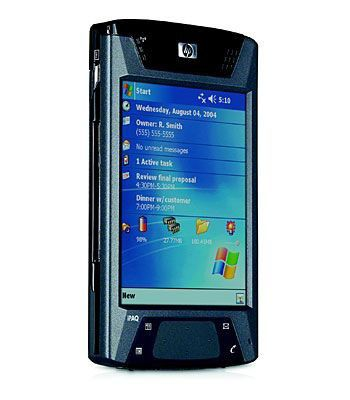
\includegraphics[width=0.3\textwidth]{Fig-19a.jpg}}
	\subfloat [Waterproof Otterbox for iPAQ]{\label{fig:19a}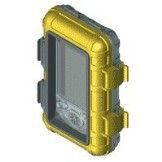
\includegraphics[width=0.3\textwidth]{Fig-19b.jpg}}
	\subfloat [GPS]{\label{fig:19a}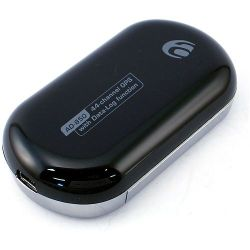
\includegraphics[width=0.15\textwidth]{Fig-19c.jpg}}
	\subfloat [Olympus waterproof camera]{\label{fig:19a}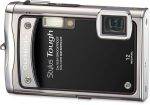
\includegraphics[width=0.25\textwidth]{Fig-19d.jpg}}
	\caption{Fieldwork equipment}
	\label{fig:18}
\end{figure}

A GPS and iPAQ have been used for detection of the geodetic coordinates and keeping the tracklogs
along the boat route for GIS project.

\begin{figure}[h]
\centering
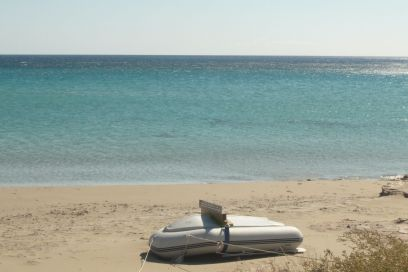
\includegraphics[scale=0.70]{Fig-18.jpg}
\caption{Boat used for the fieldwork measurements on Crete island. 2010}
\label{fig:19}
\end{figure}

\newpage

\subsubsection{Sampling design}
The sampling design of the fieldwork was aimed at surveying of the spatial distribution of the
meadows of \textit{P.oceanica}, and spatial pattern of the seagrass meadows consisted from separate
patches. The fieldwork included several routes of the boat in the Ligaria beach sampling site, nine
routes in total, in the directions parallel to the coastline, ca 180-200 m long each, thus enabling the
course plot to cover the area of growing seagrass: shelf areas not deeper than four meters.
The measurements of the seafloor cover types have been made using underwater video cameras
Olympus ST 8010, mounted under the boat to capture video footage and imagery. The data records
were made along each path using these cameras. A videographic approach, tested previously \cite{Norris97}\label{Norris97},
 was applied during the fieldwork on Crete island, for collecting information on benthic cover types and
distribution of the seagrass patches from photo transects, in order to use for the calibration of mapping approaches.
Three underwater video cameras, located on the bottom of the boat, provided videometric measurements of the
seafloor during the track, and resulted in a series of consequent overlapping images of the sea bottom under the
boat path. The general locations of the sampling sites and routes were selected on the basis of the visual examination
of the seagrass beds during snorkelling and SCUBA diving, recommendations from the Greek collaborators of the Natural Nistory Museum of Crete, and available maps covering the research area. To ensure even and objective selection of sampling sites
we used transect sampling method, i.e. photographs were taken along the research path. Transect
method is a common sampling technique in studies of the seagrass monitoring \cite{Shortis07}\label{Shortis07},
enabling the occurrences of the seagrass meadows to be recorded and counted in a systematic and
accurate way, detect spatial distribution of the single seagrass mattes to be properly identified,
without location bias. 

\begin{figure}[h]
	\centering
	\subfloat [view from below]{\label{fig:19a}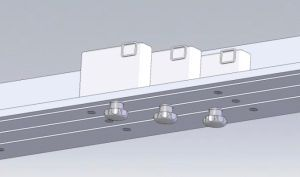
\includegraphics[width=0.3\textwidth]{Fig-20a.jpg}}
	\subfloat [view \textit{en-face}]{\label{fig:19a}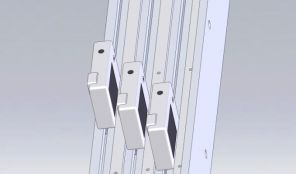
\includegraphics[width=0.3\textwidth]{Fig-20b.jpg}}
	\subfloat [view from above]{\label{fig:19a}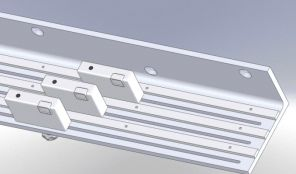
\includegraphics[width=0.3\textwidth]{Fig-20c.jpg}}
	\caption{Scheme of placements of the Olimpus cameras during the measurements}
	\label{fig:20}
\end{figure}

The videographic measurements and photos, enabling to detect types of the
seafloor, were captured by means of three underwater digital video cameras Olympus ST 8000 (Fig.\ref{fig:20}), at
five minutes interval along the tracklog path (Fig.\ref{fig:21}).
research sampling design also included measurements of depths, because bathymetry is one of the
most determinating factors for the seagrass locations. Measurements of depths were performed during
the fieldwork using cord, iPAQs, and markers in order to assure that the videometric measurements
are taken at depths not more than four meters, in the shelf area.
As a result, nine transects were established of one m wide and 20 m long track, to cover seagrass beds
with videographic measurements. The GPS allowed to capture measurement locations on the iPAQ,
encapsulated in a plastic waterproof Otterbox. Camera were adjusted horizontally by a leveller and
were mounted under the bottom of the boat to capture video footage and imagery (Fig.\ref{app:20}). The data
were taken at proper weather conditions: sunny, serene and cloud-free days with glassy sea state. The
locations of the route were randomly selected in the areas of the Ligaria beach, to ensure most dense
coverage of the seagrass meadows in the research area. The underwater measurements of the seagrass
coverage were carried out by taking video footage and photos of ca 0.5 m2 size each.
The results of the underwater videometric measurements include series of digital images helping to
classify seafloor cover types and seagrass meadows, according to the differences in the structure,
colour, texture and shapes of the depicted objects.

\begin{figure}[h]
\centering
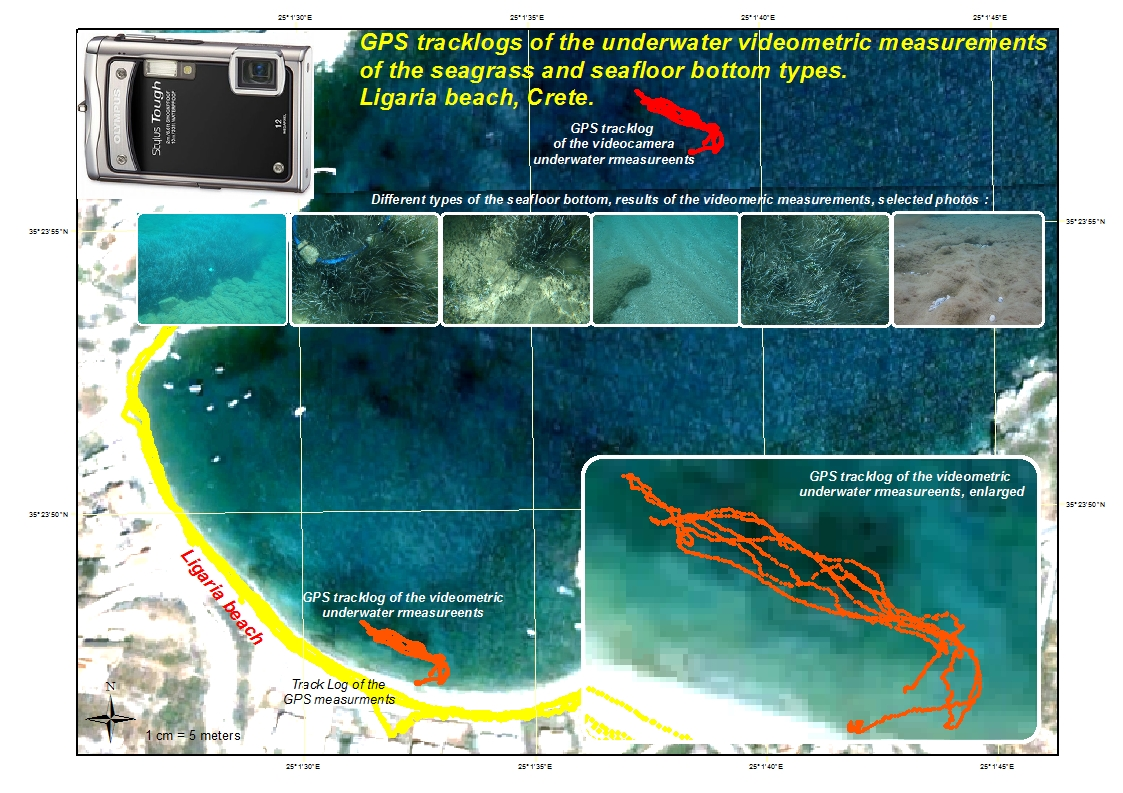
\includegraphics[scale=0.40]{Fig-21.jpg}
\caption{Locations of the video measurements and GPS tracklogs, Ligaria}
\label{fig:21}
\end{figure}

Along the Ligaria beach there are several types of the seagrass landscapes, namely, segrass meadows
continuously covering vast areas (Fig.\ref{app:18}), aggregated seagrass patches, represented by separate
mattes with short irregular channels between them (Fig.\ref{app:18}) and isolated seagrass patches, or mattes,
which located separately from broad meadows (Fig.\ref{app:18}).
The results of the underwater videometric measurements of the Olympus cameras made during the
ship route include nine total tracklog routes in the selected research area, including series of
consequent images, completely covering the area under the boat path. The received data contain
information on seagrass presence within the study area, distribution of seagrass P.oceanica meadows
and nature of the seafloor cover types (rocks, sandy, mixed). Seagrass species on the Ligaria and Agia
Pelagia beach consist of P.oceanica. The types of sediment on the Ligaria vary from coarse sand,
P.oceanica patches, sand, mud, rock gravel and fine sand (Fig.\ref{app:20}).

\subsection{Data of spectral measurements}

\subsection{Google Earth aerial imagery for seagrass mapping}
Apart from the satellite imagery, the aerial photographs from the Google Earth provide
a powerful tool for seagrass mapping, because they are important, reliable, detailed
and up-to-date source of imagery.
\begin{wrapfigure}{r}{0.5\textwidth}
\centering
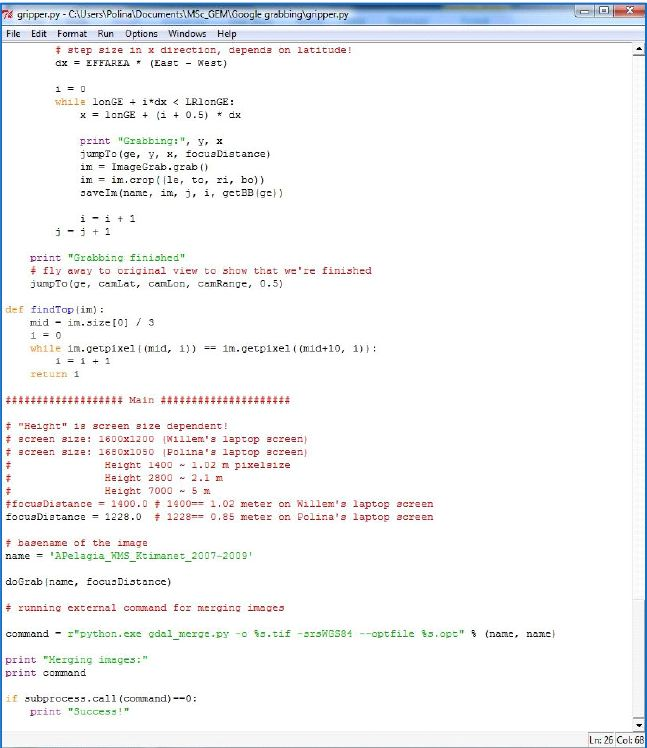
\includegraphics[scale=0.27]{Fig-22.jpg}
\caption{Capturing aerial imagery from the Google Earth: grabbing process}
\label{fig:22}
\end{wrapfigure}

Perhaps, the most clear advantage of the Google
Earth imagery is high resolution (15 m in land areas and lower in the oceans).
Obtained from the airborne platforms, Google Earth images have general spatial
resolution of several meters (though vatying in different areas), which allows very
detailed habitat and seafloor types discrimination, comparing with images
acquired from the spaceborne satellite platforms.
The spatial coverage of the Google imagery is lesser comparing to spaceborne images, but this can be solved as
well: while in general providing smaller area coverage than satellites images, the Google Earth
images can be stitched to the composite maps of the acceptable spatial extent, using Google grabbing
process which allows multiple overlapping of single images over the flight paths, and generates
mosaics.

\subsection{Application of satellite imagery for seagrass mapping (Landsat, ASTER, MODIS)}

\pagebreak
\section{Results}
%\markright{IV. Results}

\subsection{Review of the collected data}
The remote sensing imagery were collected for the Crete island area covering the research period and
area, enabling the field data to be used for the calibration and validation. The available aerial and
satellite imagery are commonly used for the mapping of seagrass landscapes and their application is
proven by various research papers. The imagery include satellite multi-spectral imagery (Landsat-TM,
ETM+) and aerial imagery from the Google Earth.
The overview of the collected data enables to summarize their following types:
1. Spectra of P.oceanica and other seafloor types at different environmental conditions
2. Aerial imagery from the Google Earth
3. Satellite images from the open sources (Landsat)
4. Underwater videometric measurements of the Olympus cameras made during the ship route
The available satellite imagery (Fig.\ref{app:20}) and aerial images are read into the ArcGIS project.
The available broadband and hyperspectral remote sensing data are used for the mapping of the
seagrass in shelf areas no deeper than 4.0 meters, for the environmental monitoring in order to detect
the dynamics in changes of the seagrass distribution along Crete during the past 10 years using
different satellite images for 2000-2010.
The spatial resolution of Landsat ETM+ image is 30 m in the visible and near infrared bands (bands
1-5 and 7); the spatial resolution of ASTER 15 m for the visible and near-infrared bands. IKONOS
acquires data in 3 visible channels and NIR, with spatial resolution of 1-4 meters. ASTER and
IKONOS images are suggested to be included as soon as available, in addition to the Landsat. The
research includes fieldwork in-situ measurements of the seagrass distribution along the northern and
south-eastern coasts of Crete in chosen locations.
The optical measurements of the irradiance and radiance of the sea water and bottom cover types of
the seafloor have been received by the means of the optical sensors Trios-RAMSES Hyperspectral
UVA/UVB Irradiance Sensor and RAMSES-ARC Hyperspectral UV-VIS Radiance Sensor (Fig.2.3
and 2.4), both adjusted for the measurements of the irradiance and radiance.
The highest measured values are located in the diapason of 410-730 nm for the water irradiance and 430-650 for the water radiance (Fig.\ref{fig:23}). 

%\begin{figure}[h]
	%\centering
	%\subfloat [Irradiance]{\label{fig:23a}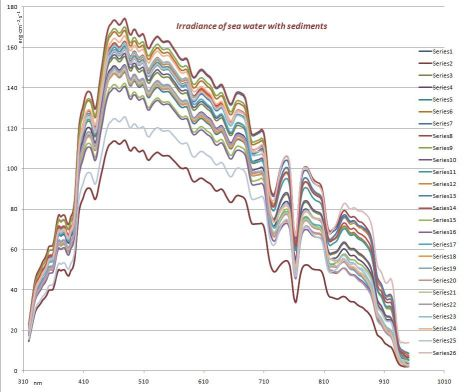
\includegraphics[width=0.8\textwidth]{Fig-23a.jpg}}\\
	%\subfloat [Radiance]{\label{fig:23b}\includegraphics[width=0.8\textwidth]{G-Radiance_Bezier.jpg}}
	%\caption{Optical properties of the sea water with sediments}
	%\label{fig:23}
%\end{figure}

Afterwards, the measured values of the
radiance and irradiance, respectively, have been used for the computation of the spectral reflectance
properties of the sea water and bottom cover types (Fig.\ref{fig:23}). The spectral range of radiance
cover diapason of 320-950 nm, and ittadiance measurements are covered in the interval of 280-500
nm, which is suitable for a characteristics of seagrass reflectance.
Different curves on the radiance and irradiance graphs (Fig.\ref{fig:23}) represent several series of
the measurements. The values of the spectral reflectance are received from the
computations of these values using Excel mathematical formulae. The graphs shown on Fig.\ref{fig:23} display values of the radiance and irradiance of the sea water in Agia Pelagia, with and
without sediments and suspended particles, respectively.
\begin{figure}[h]
\centering
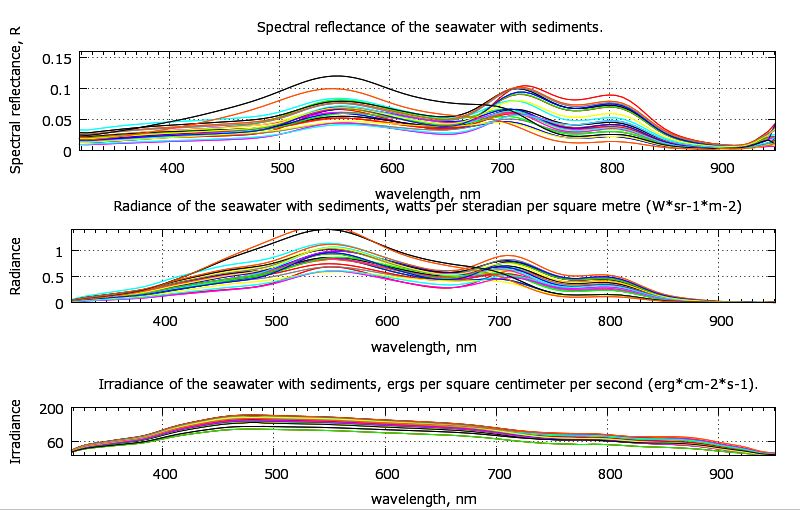
\includegraphics[scale=0.5]{GNU-17.jpg}
\caption{Optical properties of the sea water with sediments, measured in aquarium tank. Agia Pelagia district, Crete}
\label{fig:25}
\end{figure}

\subsection{Data pre-processing}
A collection of visible spectra of two seafloor cover types - \textit{P.oceanica} and carbonatic sand - were
tested for the spectral variability and separability under varying conditions of dfifferent environmental
constituents (e.g. depth, water content, sun angle etc), in order to determine the
potential that it may have on the approaches for further images processing and classification.The raw
initial data of measurements of the spectral reflectance have been preprocessed and analysed. These data
have been measured using different step of the wavebands: some measurements
were made with 3 nm interval, while others – using 4 and 1 nm step.

\begin{wrapfigure}{r}{0.6\textwidth}
\centering
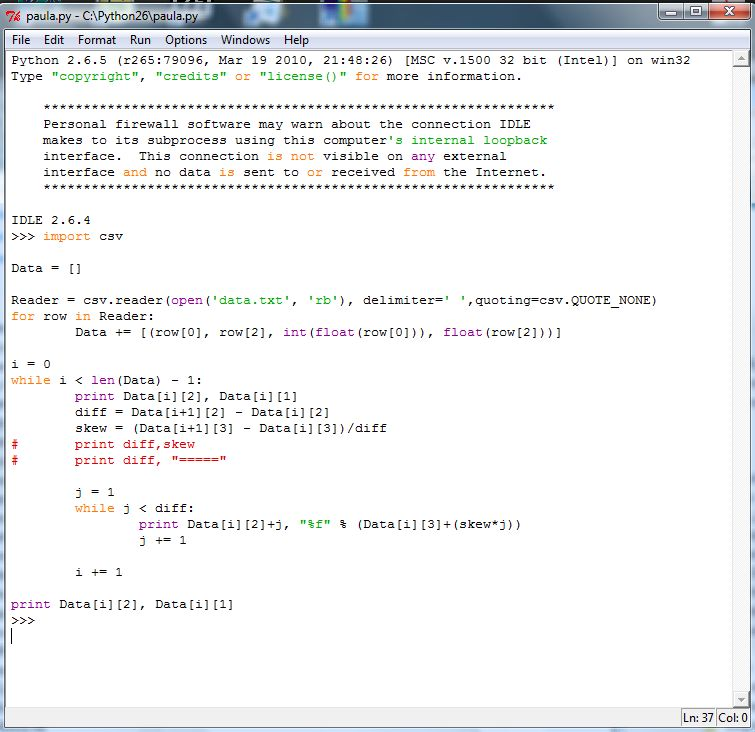
\includegraphics[scale=0.23]{Fig-24.jpg}
\caption{Script written on Python, for the interpolation raw data of the Trios-RAMSES measurements}
\label{fig:24}
\end{wrapfigure}

Therefore, these data had to be interpolated and standardized to one
format, which is values of spectral reflectancese with one nm step. For the
interpolation we used script written on Python programming language that allowed to receive more 
detailed data by interpolating them from 3 and 4 nm step up to 2 nm (Fig.\ref{fig:24}).
The interpolated data contained spectral measurements of the seagrass P.oceanica (measured at Agia
Pelagia beach, Crete), sand (measured at Agia Pelagia beach, Crete), silt and default artificial
spectrum of constant albedo at WASI (Fig.\ref{fig:25}). We included measurements of the Thalassia seagrass
(measured at Southern Chinese Sea by C.Yang \cite{Yang10} \label{Yang10}) for the comparison of the spectral reflectances of
different seagrass speciea under various environmental conditions.

\begin{figure}[h]
\centering
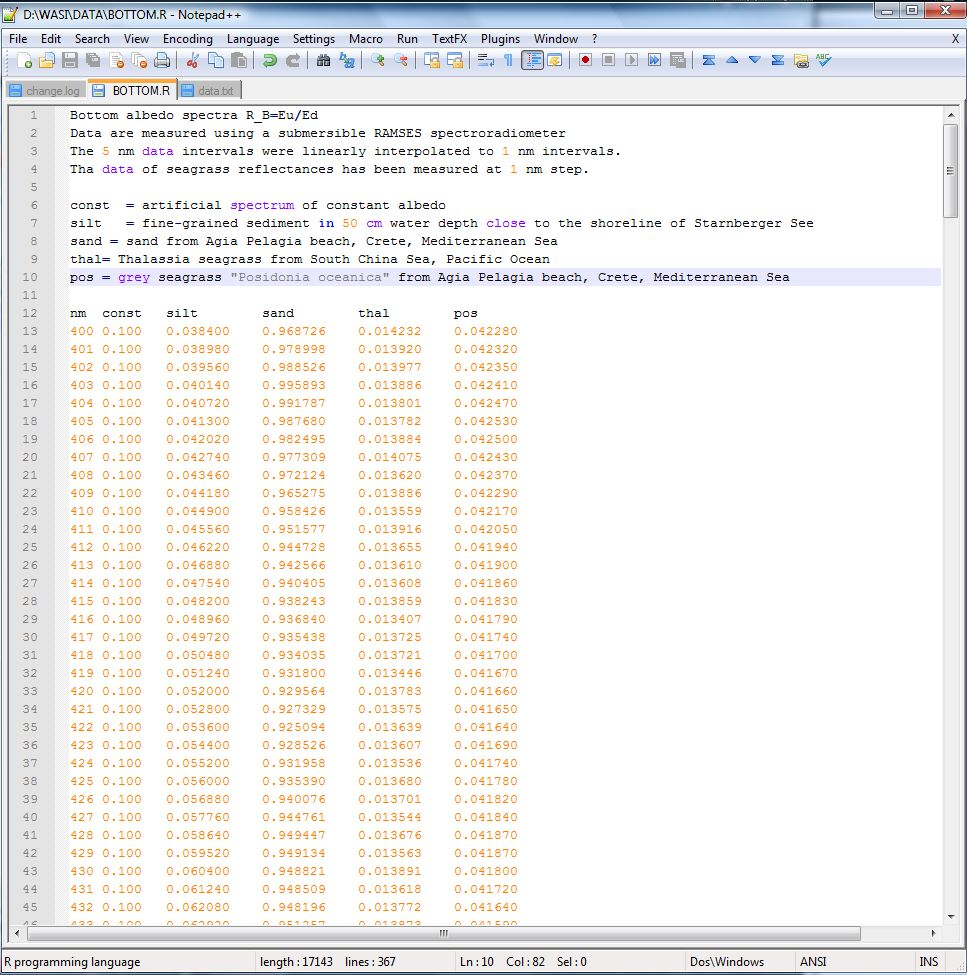
\includegraphics[scale=0.25]{Fig-28.jpg}
\caption{Fragment of \textit{Bottom.R} file: values of spectral measurements of the
seagrasses (various species), sand, silt and artificial spectrum of constant albedo}
\label{fig:25}
\end{figure}

The most suitable wavebands for the seagrass monitroring usually lay between 400 and 700 nm,
which can be concluded by the visual examination, comparison and analysis of the different spectra of
the seagrasses. Therefore, we chosen the spectra 400-750 as the most appropriate range for
further research experiment.The results of the linear interpolation (Fig.\ref{fig:25}) demonstrate values of the
sand spectral reflectances with 1 nm interval covering the wavelength diapason of 400-750 nm.\\
The initial measured data were stored in raw-oriented format, so that re-formatting them into the
column-based layout was done using “transpose” command in Open Office. The next step included
calculation of the median, mean, quartiles and other statistical values at every data set (see Appendix).
After the preliminary analysis, the measured data were visualised using GNUplot programm, which
enables fine plotting of various data. The most acceptable method of interpolation was Bézier curve ,
as it has trend-friendly graph better showing the general behavior of the curves at different wavebands
comparing to splines (see Appendix for more results). Therefore, after several experiment with
various interpolation techniques, we have choosen Bézier curves interpolation which contain convex
hulls made on its control points, and therefore is best suitable for our case: analysis of optical
properties of seawater.
\subsection{Analysis of spectral signatures}
The distinguishing spectral signatures for various seafloor types (e.g. seagrass species, coral reefs,
various types of sand, mud, other sediments, (Fig.\ref{fig:26})) exist in well-defined and narrow (10–20 nm)
wavelength ranges. 

\begin{figure}[H]
\centering
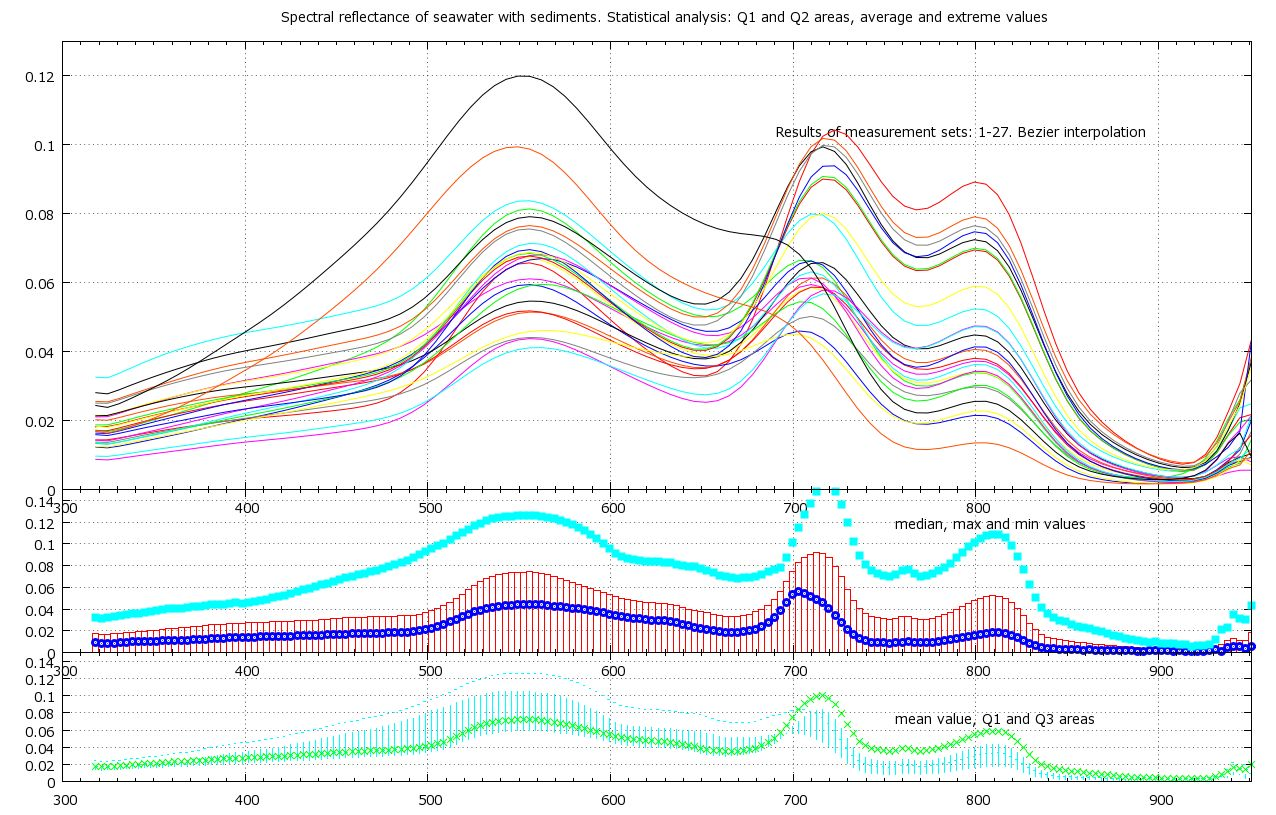
\includegraphics[scale=0.30]{GNU-18.jpg}
\caption{Multiplot graph showing spectral reflectance of the seawater with sediments, measured in aquarium tank, Agia Pelagia district, Crete. Gnuplot. \\Two complimentray graphs below show the results of the statistical analysis}
\label{fig:26}
\end{figure}

The values of their spectral reflectance are accepted as constant. The results of
spectral measurements enable to analyse, whether P.Oceanica is spectrally distinct from other sea
floor types with changing environmental conditions, using the differences in their spectral signatures
on the graphs in a WASI, the Water Colour Simulator software. \\The Water Colour Simulator WASI, a
software tool for analysing and simulating the most common types of spectra \cite{Gege05}\label{Gege05}, is highly
suitable for the seagrass spectral analysis.
There are several environmental characteristics, included in WASI interface (Fig.\ref{fig:29}), which influence the
results of water spectral reflectance, e.g. different bottom depths, concentration of suspended particles
in water column, water temperature, sun angle, concentration of gelbstoff (coloured dissolved organic
matter), concentration of phytoplankton, aerosol scattering, exponent of backscattering by small
particle \cite{Gege04}\label{Gege04}. The backward-scattering coefficient (bb), also included in WASI, is a
fundamental optical property which plays a central role in the ocean-color remote sensing, providing
the remotely sensed optical signal, as well as suspended particle distributions, water clarity, and
underwater visibility \cite{Maffione97}\label{Maffione97}. WASI enables simulation of backscattering of pure
water, large and small particles. The values of all these parameters can be redacted and changed
manuall. However, the most important, major factors affecting the in-situ conditions are water depth
and cover fraction of the seafloor types: P.oceanica and carbonatic sand (Fig.\ref{fig:27}).

\begin{figure}[H]
\centering
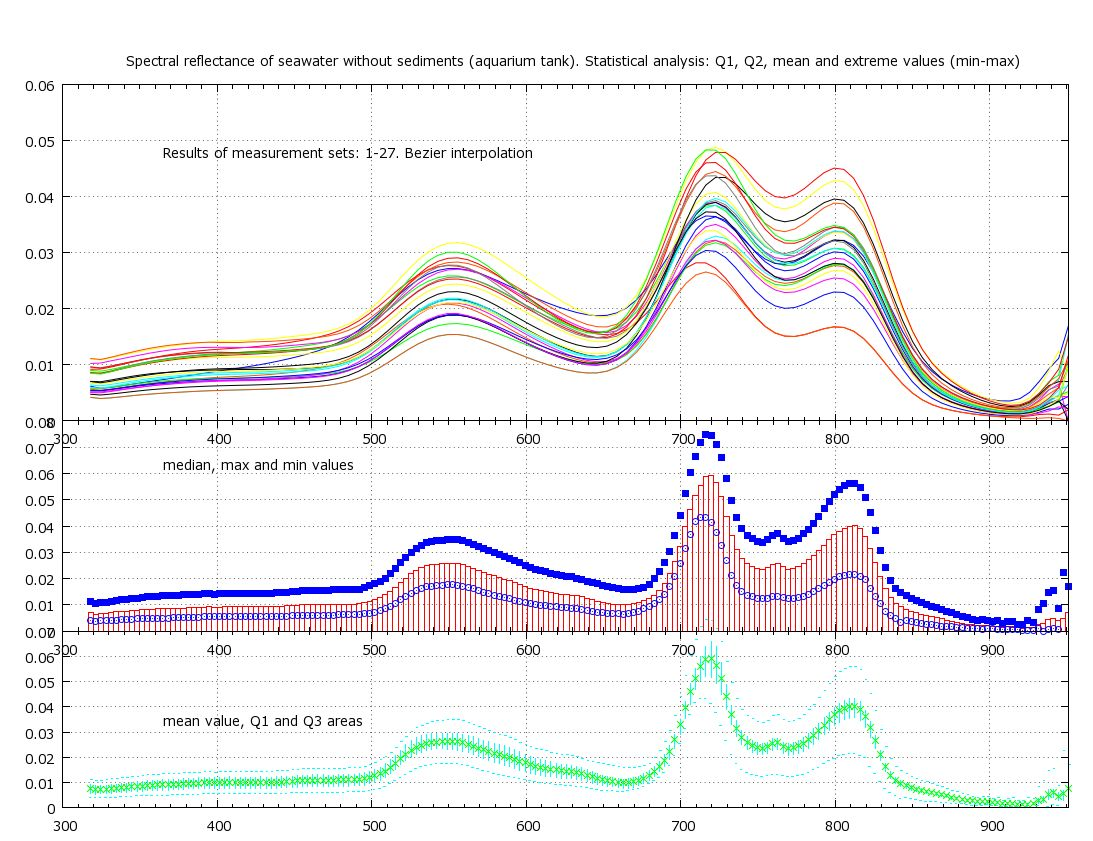
\includegraphics[scale=0.30]{GNU-21.jpg}
\caption{Multiplot graph showing spectral reflectance of the seawater without sediments, measured in aquarium tank, Agia Pelagia district, Crete. Gnuplot. \\Two complimentray graphs below show the results of the statistical analysis}
\label{fig:26}
\end{figure}

Seagrass \textit{P.oceanica} can be mapped using remotely acquired spectral imagery, if it has distinctive
reflectance signatures at different depths. Therefore, the depths of the shelf area are the first variable
condition for this research question. The depths values chosen for the current research are lesser than
3.5 meters, covering shelf zone, and providing the best enironmental conditions for the seagrass
\textit{P.oceanica}: 0.5, 2.0 and 3.5 meters with an interval of 1.5 meters. 

\begin{figure}[H]
\centering
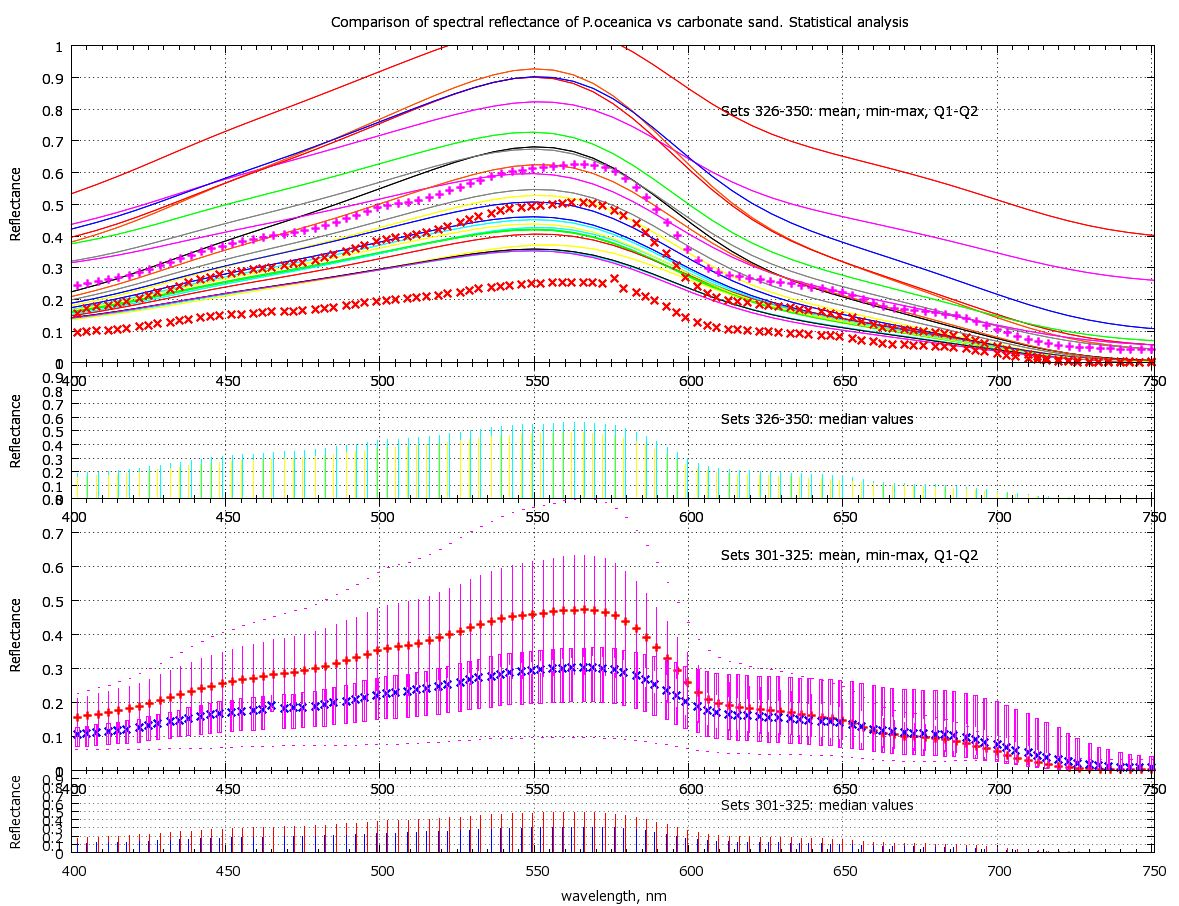
\includegraphics[scale=0.30]{GNU-20.jpg}
\caption{Statitical comparison of spectral reflectances of \textit{P.oceanica} and carbonate sand. Selected measurements sets}
\label{fig:26}
\end{figure}

The 3.5 m depth limit was chosen based on the analysis of the separability of seagrass reflectance signatures, received by the means of
previous in-situ measurements (year 2009) of the radiance and irradiance of water in Agia Pelagia
bay, which indicated that \textit{P.oceanica} seagrass could be only well separated within depths of 3.5 m.
A statistical analysis of WASI-simulated spectral reflectance has been used in order to answer the first
research question: whether the P.oceanica spectra is spectrally distinct at varying environmental insitu
conditions, and if \textit{P.oceanica} remains spectrally distinct with the increasing water column depth.
To answer this research question, different seafloor cover types are discriminated using data of the
broadband remote sensing.

\begin{table}[htbp]
\rowcolors{1}{LightSteelBlue}{Honeydew}
\caption{Results of the statistical analysis of spectral reflectance of \textbf{P.oceanica}, with average values (for sets 1 - 350). Generalisation up to step 20 nm}
\begin{center}
%\rowcolors{1}{lightgray}{white}
\begin{tabular}{|c|c|c|c|c|c|c|}
\hline
Wavelength, nm & mean & Q1 & min & Q3 & max & median \\ \hline
\textbf{318.23354} & 0.030467 & 0.038907 & 0.029764 & 0.069762 & 0.116100 & 0.048984 \\ \hline
\textbf{338.29900} & 0.033560 & 0.043030 & 0.032847 & 0.076252 & 0.128290 & 0.054334 \\ \hline
\textbf{358.37932} & 0.039897 & 0.051320 & 0.039131 & 0.091143 & 0.154409 & 0.066354 \\ \hline
\textbf{378.47247} & 0.045786 & 0.058849 & 0.045039 & 0.105993 & 0.177150 & 0.078339 \\ \hline
\textbf{398.57640} & 0.052346 & 0.066859 & 0.051625 & 0.122328 & 0.201038 & 0.091905 \\ \hline
\textbf{418.68905} & 0.058942 & 0.074842 & 0.058240 & 0.138984 & 0.226028 & 0.106207 \\ \hline
\textbf{438.80838} & 0.070690 & 0.089761 & 0.069999 & 0.167825 & 0.267712 & 0.130580 \\ \hline
\textbf{458.93235} & 0.080107 & 0.102089 & 0.079392 & 0.191424 & 0.304933 & 0.149762 \\ \hline
\textbf{479.05891} & 0.086278 & 0.110348 & 0.085546 & 0.207940 & 0.332934 & 0.162881 \\ \hline
\textbf{499.18600} & 0.098498 & 0.126592 & 0.097689 & 0.239161 & 0.380603 & 0.188192 \\ \hline
\textbf{519.31159} & 0.110222 & 0.143976 & 0.109022 & 0.265948 & 0.421370 & 0.210237 \\ \hline
\textbf{539.43363} & 0.125694 & 0.166156 & 0.124310 & 0.302678 & 0.475842 & 0.240492 \\ \hline
\textbf{559.55006} & 0.131844 & 0.175865 & 0.130257 & 0.319385 & 0.503907 & 0.253726 \\ \hline
\textbf{579.65885} & 0.121915 & 0.166084 & 0.120186 & 0.302078 & 0.485661 & 0.237873 \\ \hline
\textbf{599.75794} & 0.077236 & 0.111113 & 0.075669 & 0.200557 & 0.343876 & 0.154016 \\ \hline
\textbf{619.84529} & 0.057038 & 0.085386 & 0.055588 & 0.154781 & 0.281737 & 0.117003 \\ \hline
\textbf{639.91885} & 0.050841 & 0.077438 & 0.049432 & 0.141810 & 0.265181 & 0.106188 \\ \hline
\textbf{659.97657} & 0.038118 & 0.059971 & 0.036997 & 0.110774 & 0.223366 & 0.082411 \\ \hline
\textbf{680.01641} & 0.032892 & 0.052265 & 0.032012 & 0.095789 & 0.198389 & 0.071686 \\ \hline
\textbf{700.03633} & 0.034756 & 0.058426 & 0.033643 & 0.101504 & 0.215413 & 0.075789 \\ \hline
\textbf{720.03426} & 0.026287 & 0.047084 & 0.025162 & 0.082940 & 0.193535 & 0.061184 \\ \hline
\textbf{740.00817} & 0.009740 & 0.022355 & 0.010145 & 0.042861 & 0.132244 & 0.029414 \\ \hline
\textbf{759.95601} & 0.008651 & 0.020234 & 0.009191 & 0.039371 & 0.128165 & 0.026558 \\ \hline
\textbf{779.87573} & 0.006019 & 0.014157 & 0.006397 & 0.028320 & 0.100314 & 0.019322 \\ \hline
\textbf{799.76528} & 0.008607 & 0.020030 & 0.009050 & 0.037323 & 0.118123 & 0.026535 \\ \hline
\textbf{819.62263} & 0.008777 & 0.020295 & 0.009288 & 0.037598 & 0.118055 & 0.026799 \\ \hline
\textbf{839.44571} & 0.002562 & 0.008010 & 0.002864 & 0.017472 & 0.076515 & 0.011432 \\ \hline
\textbf{859.23249} & 0.002653 & 0.006921 & 0.002897 & 0.016121 & 0.070377 & 0.009889 \\ \hline
\textbf{878.98091} & 0.002327 & 0.008080 & 0.002821 & 0.018625 & 0.082462 & 0.011617 \\ \hline
\textbf{898.68893} & 0.004077 & 0.013098 & 0.004709 & 0.031217 & 0.101146 & 0.019767 \\ \hline
\textbf{918.35451} & 0.006215 & 0.020162 & 0.007229 & 0.045213 & 0.199711 & 0.029950 \\ \hline
\textbf{937.97559} & 0.005783 & 0.026132 & 0.007307 & 0.065475 & 0.195072 & 0.040848 \\ \hline
\textbf{951.03058} & 0.002296 & 0.026581 & 0.002380 & 0.067924 & 0.265845 & 0.041463 \\ \hline
\end{tabular}
\end{center}
\label{fig:5}
\end{table}

The results enable to study reflectance properties of the seagrass and other
seafloor types. Application of the optical radiative transfer model WASI is suggested to simulate
remote sensing sensors (MODIS, ASTER, MERIS and SeaWiFS), (Fig.\ref{fig:28}).

\begin{figure}[h]
	\centering
	\subfloat [CZCS]{\label{fig:34a}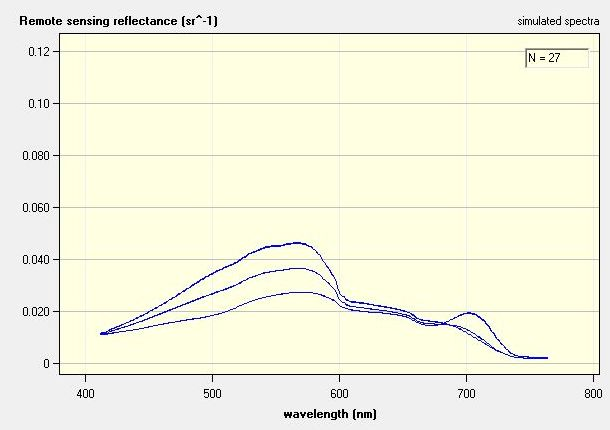
\includegraphics[width=0.4\textwidth]{Fig-35a.jpg}}
	\subfloat [MERIS]{\label{fig:34b}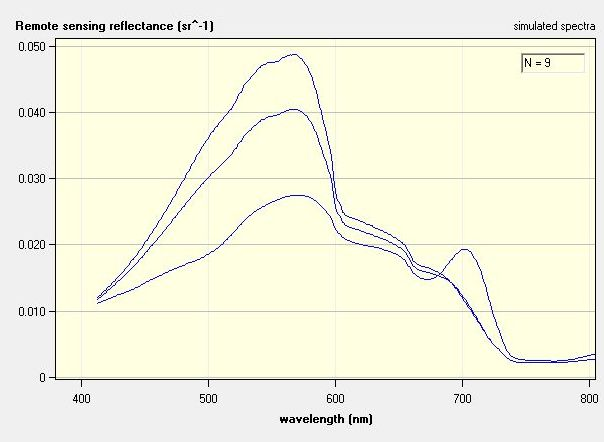
\includegraphics[width=0.4\textwidth]{Fig-35b.jpg}}\\
	\subfloat [MODIS]{\label{fig:34c}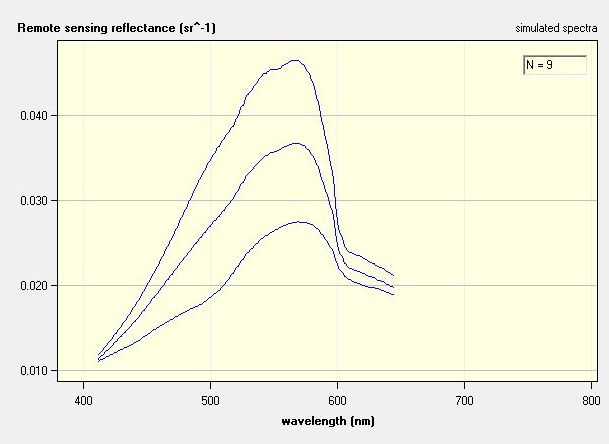
\includegraphics[width=0.4\textwidth]{Fig-35c.jpg}}
	\subfloat [SeaWiFS]{\label{fig:34d}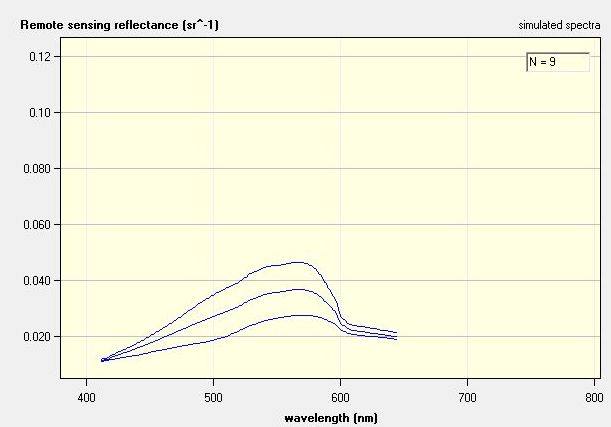
\includegraphics[width=0.4\textwidth]{Fig-35d.jpg}}
	\caption{Simulated remote sensing reflectance of \textit{P.oceanica} at various sensors}
	\label{fig:28}
\end{figure}

In order to focus on the factors of primar importance, other and less influencing factors are excluded,
i.e. sun angle, concentration of the suspected particles in the water column, content of gelbstoff, etc.
For these factors default values of WASI are accepted.
Under normal conditions by independent water colour sampling, values of the remote-sensing
reflectance can vary by 12–24 per cent \cite{Toole00}\label{Toole00}, and these variations in the radiometric
determinations are mainly caused by the variety of the environmental factors.
Different factors influence colour and spectral reflectance of water, among which different bottom
depths, concentration of suspended particles in water column, water temperature, sun angle,
concentration of gelbstoff (coloured dissolved organic matter), concentration of phytoplankton,
aerosol scattering, exponent of backscattering by small particles, cloudness, viewing geometry and
wind speed (which is, however, not the major source of uncertainty). All these environmental
components increase the absorbtion and scattering of light which, in its turn, results in a complex
relationship between their concentrations and the radiance of water that finally influence its spectral
reflectance.
However, although there are a variety of environmental factors that contribute to the spectral
reflectance, the most important ones from the mentioned above are water depth and seafloor fraction.
It is because spectra of the seagrass \textit{P.oceanica} vary qualitatively over the depths interval of 0.5–4 m,
and secondly, the content and cover fraction of the seafloor have the most distinctive effect on the
spectral reflectance of the water.
Therefore, in current MSc research we focus on these two major factors, and study the response of the
water reflectance towards changing conditions of the water column depth and seafloor bottom cover
fraction (seagrass P.oceanica, carbonate sand and silt).
The analysis of the spectral signatures of the seagrass and sand clearly shows (Fig.\ref{fig:27}) that seagrass
has spectral reflectance much lesser than that of a carbonate sand, in general not increasing values of
10 percent reflectance in spectra of 500-600 nm, while sand has spectral reflectance approaching 33 percent in its
highest values.

\subsubsection{Water color spectral simulation using WASI}
The main aim of this part of research is to clarify if the bottom reflectance of the different seafloor types including patches of
the seagrass \textit{P.oceanica}meadows, silt and carbonate sand differ and can be clearly discriminated while mapping. A study is
based on three seafloor types containing silt, carbonate sand and seagrass, as well as mixed
types, where the spectral signatures were examined. WASI software (Fig.\ref{fig:29}) is used to simulate
spectral reflectance and colour discrimination of water, affected by presence of \textit{P.oceanica} and other factors, under various
environmental conditions which influence its colour.

\begin{figure}[h]
\centering
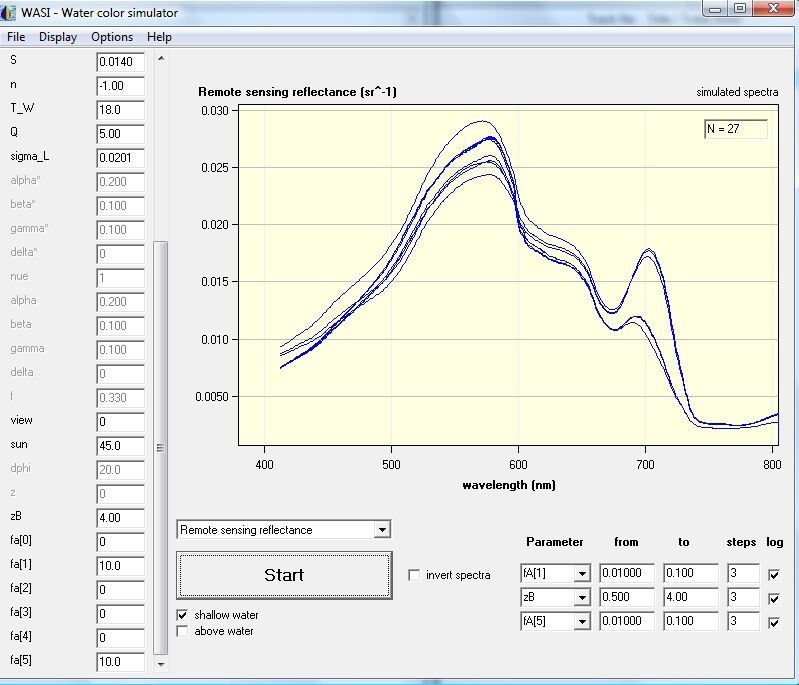
\includegraphics[scale=0.30]{Fig-30.jpg}
\caption{Main interface of WASI water color spectral simulation: \\ Spectral reflectance of \textit{P.oceanica} and silt at 0.5-
4.0m}
\label{fig:29}
\end{figure}

The data provided with the model was determined at freshwater of the Boddensee \cite{Gege05}\label{Gege05}, 
yet the model was adjasted for the marine
environment, so that its parameters (concentration of chlorophyll, concentration of small particles,
yellow substance, etc) now perfectly simulate the Mediterranean water conditions.
The remote sensing reflectance has been compared under the conditions of different water depths and
cover fraction of the seafloor, in order to assess spectral signatures of the seagrass and carbonate sand
as major seafloor types. WASI enables to use forward or inverse calculation for the spectrum types at
a diapason of 350-800 nm with a 1nm spectral resolution. For the spectral analysis we applied
forward calculations, which is a computing and plotting of series of spectra according to specified
parameter settings, with exactly defined depths and cover fraction.
The specific parameters chosen for the simulation of the environmengal conditions where seagrass
grow. The adaptations to life in salt sea water requires various phisical and chemical parameters
which include salinity, temperature of 17-25°C, light requirements with 10-20 percent on average, ranging
from 4.4percent  minimal up to 29 percent \cite{McKenzie09}\label{McKenzie09}, so that the zenith angle is taken as 35-
45° and reflection factor 0.0201. P.oceanica. 
The calculations are done for the spectrum 350-800 nm, covering the most important part of the RS spectrum: 1) Blue-green 0.45 - 0.5 μm; 2) Green 0.5 - 0.6 μm; 3) Red 0.6 - 0.7 μm; 4) Red-NIR 0.7 - 0.8 μm (Fig.\ref{fig:30}).

\begin{figure}[h]
	\centering
	\subfloat [Concentration of Gelbstoff at depths 0.5 – 8.0 m]{\label{fig:31a}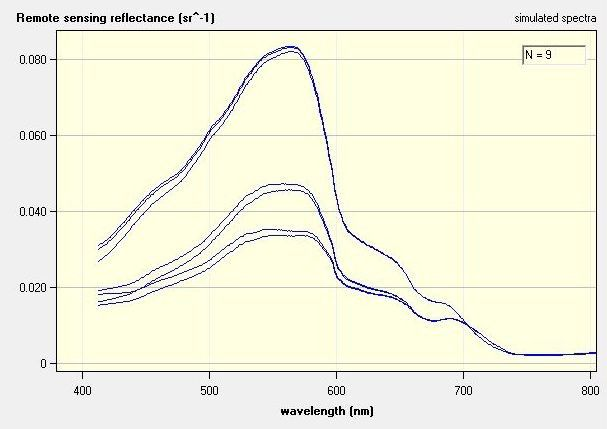
\includegraphics[width=0.4\textwidth]{Fig-31a.jpg}}
	\subfloat [Bottom reflectance at depth 0.5-4.0 meters]{\label{fig:31b}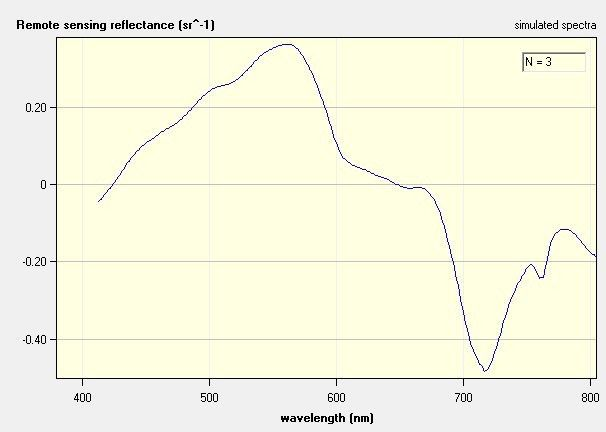
\includegraphics[width=0.4\textwidth]{Fig-31b.jpg}}
	\caption{Sea water physical properties, modelled by WASI}
	\label{fig:30}
\end{figure}
\paragraph{Model parameters: depth and bottom cover fraction}
Although seagrass \textit{P.oceanica} can be found until depth limits down to 40 m depth (Hartog
1970), the most preferrable limits of its distribution in the Mediterranean Sea are shallow waters until
4 meters of depth. 

\begin{table}
\rowcolors{1}{Aquamarine}{Azure}
\caption{Model-specific parameters of water WASI adjusted to simulate environment of the Mediterranean Sea along Crete}
\centering
%\rowcolors{1}{lightgray}{white}
% \scalebox{0.7}
  \begin{tabular}{|  p{2cm} | p{6cm} | p{25mm} | }
    \hline
    \textbf{Parameter, WASI} & \textbf{Name and description} & \textbf{Values} \\ \hline\hline
    C-L & Concentration of large suspended particles & 8 \\ \hline
   C(i), i=0..5 & Concentration of Phytoplankton & 0.035 -0.089 ug -l \\ \hline
    bbS & Specific backscattering for small particles & 0.005 m2g-1 \\ \hline
   T-W & Temperature of water & 17-25 °C \\ \hline
    n & Exponent of Backscattering by small particles & 0.005 m2g-1 \\ \hline
    Q &Anisotropy factor of upwelling radiation ("Q-factor") & 5.00 \\ \hline
    sigma-L & Reflection factor of sky radiance & 0.0201 \\ \hline
    b1 & Backscattering coefficient of saline waters & 0.00144 m-1 \\ \hline
    λ0 & Reference Wavelength for Gelbstoff absorption & 440 \\ \hline
    sun & Sun zenith angle & 45.0 \\ \hline
    zB & Bottom depth & 4.00 \\ \hline
   f(i), i=0...5 & Areal fraction of bottom surface type number n & 01/10/10 \\ \hline
    K0 & Coefficient of Attentuation & 1.0546 \\ \hline
   view & Viewing angle (0 = nadir) & 0\\ \hline
    C-X & Concentration of non-chlorophyllous particles (absorption at λ0) & 0 \\ \hline
   λS & Reference wavelength for scattering of small particles & 500 \\ \hline
    C-S & Concentration of small suspended particles & 0 \\ \hline
   S & Exponent of Gelbstoff absorption & 0.0140 \\ \hline
    C-Y & Concentration of Gelbstoff (absorption at λ0) & 0.400 \\ \hline
    Bn & BDRF of bottom reflectance (sand) & 0.318 sr -1\\
    \hline
  \end{tabular}
   \label{table:1}
\end{table}

The increase of depths (zB) influences weakening of light and thus directly affects
production of chlorophyll, because when light passes through the water and suspended particles, it is
being largely modifed through the absorption and scattering before it finally reaches plant canopy of
the seagrass. Therefore, the most healthy and suitable areas for the seagrass grow are located at depths
lesser than 4 meters (Fig.\ref{fig:31}).

\begin{figure}[h]
	\centering
	\subfloat [depth of 0.5 m]{\label{fig:32a}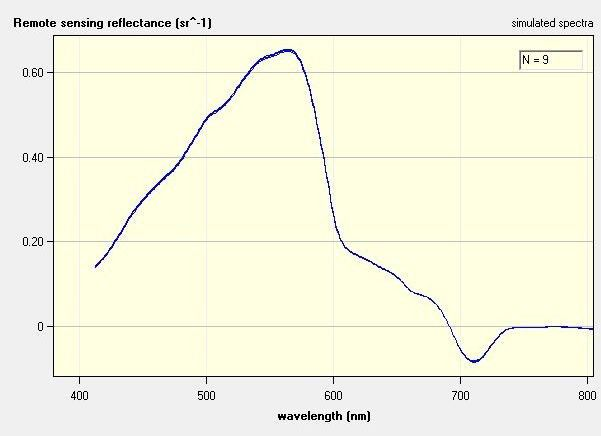
\includegraphics[width=0.4\textwidth]{Fig-32a.jpg}}
	\subfloat [depth of 2.0 m]{\label{fig:32b}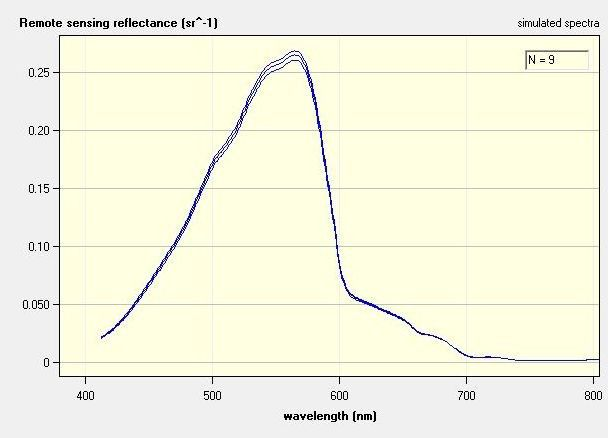
\includegraphics[width=0.4\textwidth]{Fig-32b.jpg}}\\
	\subfloat [depth of 3.5 m]{\label{fig:32c}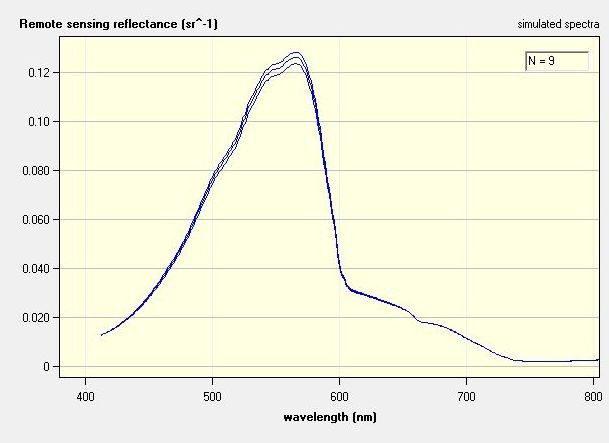
\includegraphics[width=0.4\textwidth]{Fig-32c.jpg}}
	\subfloat [depths of 0.5, 2.0 and 3.5 m]{\label{fig:32d}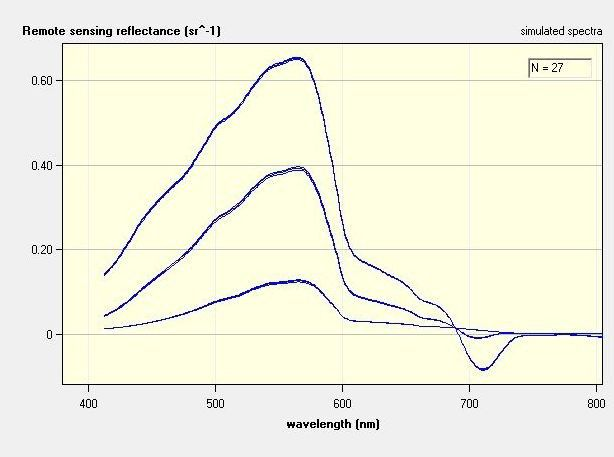
\includegraphics[width=0.4\textwidth]{Fig-32d.jpg}}
	\caption{Remote sensing reflectance of \textit{P.oceanica} at various depths}
	\label{fig:31}
\end{figure}

An analysis of the spectral reflectances of \textit{P.oceanica}.is done using the WASI simulations in order to
determine, which wavebands can be still used to identify \textit{P.oceanica}. The analysis of spectra shows
that the appropriate wavebands for seagrass mapping lay between 500 and 600 nm and has
also peaks at around 700 nm, ca between 680 and 710 nm (Fig.\ref{fig:31}). The highest values of the bottom
reflectance are at spectra of 500-600 nm. The most appropriate depths at which the spectral signatues
could still be discrtiminated for seagrass are lesser than 2.5 meters.
The remote sensing properties of the broad-band satellite sensors are often limited and do not allow
easy and unique discrimination of seagrass from other seafloor tyeps. Therefore, we focus on narrowband
spectra with the resolution of 1 nm.

\paragraph{Spectral discrimination of \textit{P.oceanica}}
The patches of white sandy bottoms of the seafloor, studied in the fieldwork in Ligaria beach, are
much brighter than mattes of P.Oceanica ((Fig.\ref{app:30}): bottom types in Ligaria), which can be clearly seen
at the graph comparing values of the spectral reflectance of the carbonate sand and than that of P.
oceanica (Fig.\ref{fig:33}).

The graph is received in excel spreadsheet using mean values of spectral reflectances of
sand (Fig.\ref{fig:34}) and seagrass (Fig.\ref{fig:32}), respectively, which have been calculated from measurements of radiance and
irradiance received in Agia Pelagia bay.

\begin{figure}[h]
\centering
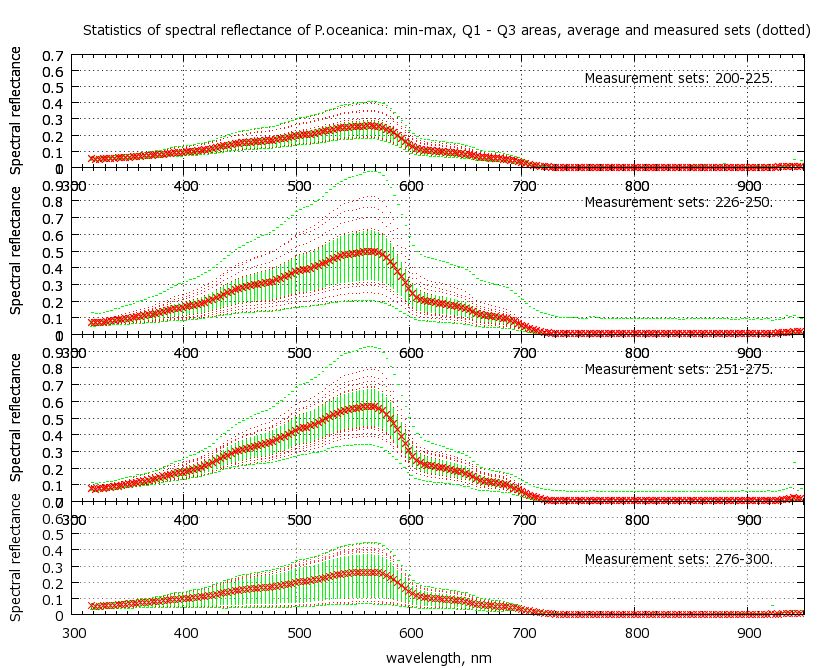
\includegraphics[scale=0.40]{GNU-19.jpg}
\caption{Statistical analysis of the spectral reflectance of \textit{P.oceanica}: min-max, average values (red bold points), Q1-Q3 areas (green vertical dashed) and measured values (dotted): multiplot of measurement sets 200-300}
\label{fig:29}
\end{figure}

\begin{figure}[h]
	\centering
	\subfloat [Sand]{\label{fig:27a}\includegraphics[width=0.4\textwidth]{Fig-27a.jpg}}
	\subfloat [\textit{P.oceanica}]{\label{fig:27b}\includegraphics[width=0.4\textwidth]{Fig-27b.jpg}}
	\caption{Bottom albedo of carbonate sand and \textit{P.oceanica}, Agia Pelagia}
	\label{fig:33}
\end{figure}

\paragraph{Spectral discrimination of sand}

\subsubsection{Statistical analysis of the observational data and hypothesis testing}
The raw data of measurements of spectral reflectances of P.oceanica have been tested statistically. We
analysed 400 datasets made on two different data.
The total amount of measured data was large and included following datasets made using
hyperspectral radiometer Ramses: 350 measuremetn sets of P.oceanica reflectance for 14th Oct, 400
sets of P.oceanica reflectance for 15th Oct, 84 datasets for seawater reflectance with sediments, 105
datasets for seawater reflectance without sediments, 87 sets for spectral reflectance of carbonat sand.
Fig. 4.11. Spectral reflectance of water with sediments
Therefore, a statistical approach is necessary for the processing of such data. Statistical pre-processing
of large sets of serial data enables to generalyse data by using the most typical and predicted values of
spectral reflectance for further calculations, and to get rid of the extreme values, noise and errors.
The statistical calculators were made by means of Open Office and included following computations
at each data set (table 1): mean, median, Q1 and Q3, standard deviation, min and max values. The
statistical pre-processing and analysis were made shown the mean values of spectral reflectances,
which were used for comparison with reflectance data of various seafloor cover types as well as
seawater with and without sediment.
The visualization of the data plotting was made by means of Gnuplot software, which enabels fine
drawing and advanced displaying of large amounts of serial data, ultimate control over graph properties, 
the simplicity of plotting and the ease of scripting. (see Fig.15 and Appendix).
The graphs illustrating spectral signatures of various seafloor cover types display the mean values and
areas of quartiles (Q1, Q3, shaded areas on graphs), which cover most probable data distribution
(spectral reflectance) for each spectral band. In x-axis I displayed the areas of 400 – 950 nm in
spectra, where the measurements were done; the y-axis was adjusted for the better visualisation of the
P.oceanica spectra: as its spectral values are mostly located in the lower part of the spectra (usually no
more than 0.20 nm, except for borders), I did not extend the y-scale up to 100 percent, in order to
focus on the most necessary area of spectral values (Fig. 15 and Appendices). The mean values are
highligted using bold points, as I used these values for plotting the final graph of P.oceanica spectra in
Ligaria beach, Agia Pelagia.
\begin{figure}
\begin{center}
\includegraphics[scale=0.45]{GNU-13.jpg}
\caption{Multiplot of spectral reflectance of P.oceanica. Series 1-100. Shown midspread of the statistical quartiles Q1 and Q3 (vertical dashes) and
mean value within the range (red bold dots). Gnuplot visualization­}
\label{app:1}
\end{center}
\end{figure}
\begin{figure}
\begin{center}
\includegraphics[scale=0.5]{GNU-16.jpg}
\caption{Multiplot of spectral reflectance of carbonate sand. Series 1-75. Shown midspread of the statistical quartiles Q1 and Q3 (vertical dashes) and
mean value within the range (red bold dots). Gnuplot visualization­}
\label{app:1}
\end{center}
\end{figure}

A statistical hypothesis test has been applied for the making decision and controlling the wealth of the
observational data of of the hyperspectral measurements of the water reflectances.
The received results are statistically significant if they are unlikely to have occurred by chance alone,
according to a pre-determined threshold probability, the significance level. Therefore, we applied
critical tests of significance to analyse the measured data according to their significant value.
Answering the first research question, we suggest the following statement.
Assuming that the null hypothesis, Hypothesis Ho, is true, which is “the spectral distinguishability of
the seagrass P.oceanica from other seafloor types is not changing with varying in-situ conditions,
Ho: μ1 =μ2 =μ3=...= μn.”, what is the probability of observing the values of spectral reflectance of
P.oceanica at various depths, for the test statistic, that is at least as extreme as the values of spectral
reflectance of P.oceanica at these depths, that was actually observed? The alternative Hypothesis Ha
Fig.15. Multiplot display of spectral reflectances of P.oceanica. Measurement sets 1-100, 15th
October. Bold red dots show the mean values within each dataset; vertical areas: quartiles Q1-Q2.
claims the opposite statement: “the spectral discernibility of the seagrass P.oceanica is distinctly
changing with varying in-situ conditions, i.e. increasing depth, Ho: μ$\neq$μ2$\neq$μ3$\neq$ ... $\neq$μn“.
Two statistical approaches have been tested for confirmatory data analysis and hypothesis testing.

\paragraph{ANOVA-testing}
The ANOVA (ANalysis Of Variance) testing is applied for the analysis of the probability of the
spectral reflectance of P.oceanica to be more or less spectrally disticnt from other seafloor cover
types with changing depth. W are checking the statement Hypothesis Ho, is true, which is “the
spectral distinguishability of the seagrass P.oceanica from other seafloor types is not changing with
varying in-situ conditions, Ho: μ1 =μ2 =μ3=...= μn.” which gives the following outcome.
P(reject H0|H0 is valid)= P(X>c|p=)=.05
where c comes for critical values and p=probability.
The result P=.05 is, hence, very small, which makes the statement of Hypothesis Ho highly unlikely
(less than 1 in a 10 chance). The one-way ANOVA highlighted a significant difference between data
of spectral reflectances of P.oceanica at different depths, i.e. true is the opposite statement:
Hypothesis Ha=“the spectral discernibility of the seagrass P.oceanica is distinctly changing with
varying in-situ conditions, i.e. increasing depth, Ho: μ$\neq$μ2$\neq$μ3$\neq$ ... $\neq$μn“.

\paragraph{Student-t testing}
The Student-t test is one of the most commonly used techniques for testing a hypothesis on the basis
of a difference between sample means. In our case the Student t-test demonstrates if the variation
between two analysed groups – values of spectral reflectances of seagrass P.oceanica and sand - is
significant. Therefore, we use Student t-test to compare two sets of quantitative data of spectral
reflectances of P.oceanica and sand, respectively, with samples collected independently of one
another. The Student-t test can be performed knowing just the means, standard deviation, and number
of data points. Therefore, we used the data (Appendix 11) of means of spectral reflectances of both
bottom cover types within data sets, their standard deviation, and the number of data points.
The results show the following outcome.
As a result of the statistical testing, we came to the following conclusion.
The Hypothesis Ha is true, which claims that the spectral discernibility of the seagrass P.oceanica is
distinctly changing with varying in-situ conditions, i.e. increasing depth, Ho: μ1≠μ2≠μ3≠...≠ μn .
Statistical results are illustrated with Error bars made using Excel's vertical box and Whisker Charts
(Box Plots, Fig..).
The graphs werer plotted on the basis of the following statistical data calculated from the sampling
measurements data: Table 2.

\begin{table}
\rowcolors{1}{Khaki}{LightYellow}
\caption{Statistical analysis of the measurements of spectral reflectance of P.oceanica (fragment).}
\centering
  \begin{tabular}{| c | c | c | c | c |}
    \hline
    \textbf{Statistical values} & \textbf{318.19} & \textbf{418.3448} & \textbf{518.8361} & \textbf{619.3662} \\ \hline \hline
    Mean & 0.034521 & 0.049235 & 0.076088 & 0.085287 \\ \hline
    St Dev & 0.019849 & 0.030338 & 0.042587 & 0.046569 \\ \hline
   Median & 0.033035 & 0.046197 & 0.07704 & 0.080277 \\ \hline
   Q1 & 0.019293 & 0.023706 & 0.045606& 0.049468 \\ \hline
   Q3 & 0.042477 & 0.057934 & 0.092289 & 0.114191 \\ \hline
   Minimum & 0.007898 & 0.010087 & 0.021373 & 0.022691 \\ \hline
   Maximum & 0.076835 & 0.110906 & 0.18938 & 0.216231 \\ \hline
   25th Pct & 0.019293 & 0.023706 & 0.045606 & 0.049468 \\ \hline
   50th Pct & 0.013743 & 0.022491 & 0.031435 & 0.030808 \\ \hline
   75th Pct & 0.009441 & -0.01174 & -0.01525 & -0.03391 \\ \hline
   Min & 0.011395 & 0.013618 & 0.024232 & 0.026777 \\ \hline
   Max & 0.034358 & 0.052972 & 0.097091 & 0.1 \\ \hline
  \end{tabular}
   \label{table:1}
\end{table}

where the abbreviations stand for the following values:
Mean: Average of the data to be plotted, AVERAGE {data}
St Dev: Standard deviation, STDEV{data}
Median: Median of the data, MEDIAN{data}
Calculating interquartile ranges: Q1=First quartile, PERCENTILE({data}*0.25) and Q3=Third
quartile, PERCENTILE({data}*0.75)
Minimum: Minimum value,MIN{data}
Maximum: Maximum value, MAX{data}
25th Pct: Plotting value of first quartile = Q1
50th Pct: Plotting value of median = Median-Q1
75th Pct: Plotting value of third quartile = Median-Q3
Min: Lower error bar lenth=Q1 - Minimum
Max: Upper error bar lenth=Maximum - Q3
The statistical analysis is displayed on the Graph 1.1 which compares the spread in sets of
measurement data of spectral reflectances of under various environmental conditions (depth).

\subsubsection{Results of the remote sensing application}
The in situ spectral reflectance data of \textit{P.oceanica} and sand were used to model these seafloor cover
types as the different sensors would percept them: MODIS, ASTER, MERIS, SeaWiFS and CZCS.
These models simulate spectral views of the chosen sensors, how these sensors will "see" seagrass (Fig.\ref{fig:28}) and sand as
pixels, with accepted default atmosphere and water column effects (given by WASI software). In such
a way we defined an empirical upper limit to the discriminative potential of these sensors. To create
these sensor-specific reflectance spectra, spectral responses of each of these sensor were applied for
the spectral signature of seafloor cover types in full-resolution spectra.

\pagebreak

\subsection{Image processing using Erdas Imagine}
The analysis of the imagery of Cretan coasts is based on the images classification and is aimed to
investigate the distribution of the seagrass P.oceanica within the research area.
In the image processing part of the research supervised classification has been applied to the aerial
and satellite images. Seagrass meadows and other seafloor cover types were evaluated through a
detailed examination of the imagery. \\
Seagrass beds are clearly visible in color aerial Google Earth
photographs (Fig.\ref{fig:35}), contrasting against slightly-yellow and browny sand bottom. The seagrass areas are
detected using different bands combinations, masked and studied for the estimation of the changes in
the areas. The classification is based on the spectral properties of the \textit{P.oceanica}, such as brightness,
colour, texture and structure of the seagrass mattes (Fig.\ref{fig:35}a). The raster-based mapping
includes supervised classification with training sites of seagrasses (10-15 set areas) in different bands
for each photograph by classification a series of polygons characteristic of each of the sea floor
bottom types: sandy surface, seagrass bed for each species including \textit{P.oceanica} (meadows), patchy
seagrass bed and algae on rock, rocks, muddy surface, etc (Fig.\ref{fig:36}).

\begin{figure}
	\centering
	\subfloat [small-scaled (1:54,000)]{\label{fig:35a}\includegraphics[width=0.8\textwidth]{Fig35a.jpg}}\\
	\subfloat [enlarged (1:10,000)]{\label{fig:35b}\includegraphics[width=0.8\textwidth]{Fig35b.jpg}}
	\caption{Seafloor types of the Arina beach: \textit{P.oceanica} sand, rocks}
	\label{fig:35}
\end{figure}

On the basis of the image processing and classification, applied to the northern coats of Crete, the
marine bottom types between 10 m depth has been mapped, including the limit depths of the of the
seagrass meadows provided on the basis of the available and collected field data. The classification
has been completed using ENVI and Erdas Imagine software.

\begin{figure}
\begin{center}
\includegraphics[scale=0.40]{Fig-36.jpg}
\caption{Results of the image classification in Erdas Imagine: seagrass distribution in Bali area, Crete}
\label{fig:36}
\end{center}
\end{figure}

\subsection{Seagrass mapping using ArcGIS}

\subsubsection{Data integration}
The integrated approach used in this research work has high potential as a means to monitor changes
in seagrass landscape occurring in a shallow waters over Crete area.

\begin{figure}
\begin{center}
\includegraphics[scale=0.25]{Fig-37.jpg}
\caption{Google aerial images incorporated into the GIS project: fragment of ArcMap layout}
\label{fig:37}
\end{center}
\end{figure}

It encompasses the integration of
high resolution aerial color Google Earth photography, spaceborne satellite imgery, assessment of
spectral signatures using WASI software, image processing by means of Erdas Imagine (Fig.\ref{fig:39}) and Arc GIS
based mapping. The use of GIS for data incorporation (Fig.\ref{fig:37}), storage, analyses, visualizing and mapping
enables to analyse environmental changes within seagrass landscapes based on data from various
sources: aerial and satellite images, geographically referenced maps of Crete island and results of
images classification showing areas of seagrass distribution.
The final mapping has been supported in ArcGIS through the data exporting, conversion and
integration of various data in one GIS-project. Data collected during the fieldwork, imagery
of the seagrass distribution are added into a GIS dataset for the assessment and spatial analysis.

\subsubsection{Upscale mapping of the seagrass landscapes}
Although ocean pelagic landscapes have a high degree of spatial variance and less structurally
complex, comparing to the terrestrial ones, the landscape-level phenomena have similar features, and
there are accepted definitions of landscapes elements within the seagrass meadows \cite{Robbins94}\label{Robbins94}. 
In general, the structure of seagrass landscape is more simplier than that of the terrestrial
ecosystems in biodiversity and complexity, however, seagrass landscapes show variation in spatial
patterns over different special scales. Complexity of the landscape of seagrass meadow show the
measure of patches in size and shape, expressed in ratio of patch perimeter to area. The fragmentation
of the seagrass landscapes is expressed in contiguity displaying patch aggregation within meadows.\\
The general principles of the hierarchy within the seagrass landscapes are based upon the quantitative
analysis of the spatial patterns, consisted by components and separate elements. Thus, the bunches of
individual shoots construct patches, the first hierarchical level. Patches are arranged into discrete
clumps of mattes (at a scale of centimeters to meters) which, in turn, make up beds with l-100m in
diameter. Finally, seagrass beds, are arranged into meadows that may extend over kilometer-wide
areas, historically defined as landscapes \cite{Robbins94}\label{Robbins94}.

\begin{figure}[h]
	\centering
	\subfloat [Meadows of the seagrass. Source: Googel Earth]{\label{fig:38a}\includegraphics[width=0.4\textwidth]{Fig-38a.jpg}}
	\subfloat [Patches (mattes) of the seagrass. Source: in-situ videometric measurements]{\label{fig:38b}\includegraphics[width=0.47\textwidth]{Fig-38b.jpg}}
	\caption{Variations in spatial structure of the seagrass landscapes}
	\label{fig:38}
\end{figure}

Besides spatial structure of the seagrass meadows, there are strong and complex patterns of depth zonation, specific fo individual
seagrass species, but such detailed clasiification goes beyond the scope of the current MSc research.
Unique feature of seagrass meadows, most characteristic for shallow areas, is dynamics of their
landscapes. Homogeneous, continuous seagrass meadows can reach in size up to 40 m2 (Fig.\ref{fig:38} a),
however they are often interrupted by gaps and channels of open spaces generated by the complex,
disturbin sedimentation processes, turbulence and turbidity regime of waters and landscape dynamics,
which form gaps and channels within meadows, making them “patchy-looking”, i.e. diversified by
separate mattes (Fig.\ref{fig:38} b). The traditional definition for gap in vegetation cover is “disturbancegenerated
openings in either floral or faunal cover” \cite{Connell78}\label{Connell78}.

\begin{figure}[h]
\begin{center}
\includegraphics[scale=0.25]{Fig-39.jpg}
\caption{Results of the unsupervised classification of the seafloor cover types and land structure, Agia Pelagia; raster layer read into the ArcGIS project}
\label{fig:39}
\end{center}
\end{figure}

Formation and increase of these
gaps within the mosaic of seagrass meadows is caused by different reasons. The most probable
drivers for the process of gaps formation within seagrass meadows are removal of interior vegetation,
differential growth of seagrass meadows and increased sedimentation. Thus, storms lead to severe
deposition of sediments, burying parts of seagrass meadow, the same effect has movements and
deposition of sediments during and after floods\cite{Bell99}\label{Bell99}.
Increased nutrient sedimentation, expecially phosphorus, were explored \cite{Jensen01}\label{Jensen01} as a
potential mechanism for increasing patch dynamics and morphological plastisity within seagrass
meadows. Finally, increasing the degree of fragmentation of the landscapes of P.oceanica meadows
can be caused by the invasion of alien species, such as Cymodocea nodosa, Caulerpa prolifera,
Caulerpa taxifolia. Invaders are in general strong colonizers comparing to native P.oceanica: they
occupy much greater habitat space within the regressed meadows of stressed native seagrass
\cite{Montefalcone10}\label{Montefalcone10}. However, on the northern coasts of Crete the only dominating seagrass
species is P.oceanica.
Morphological differences in scale of seagrass landscape formations, discussed above, cause need for
the different-scale mapping. Therefore, the investigation of the seagrass meadows at different levels is
performed using underwater videometric measurements, aerial and satellite imagery.

\pagebreak

\subsubsection{Results of GIS mapping}
This research part results in series of thematic maps showing seagrass spatial distribution over the Island of
Crete. The research is based on the aerial images classification and analysis using ArcGIS and Envi
software (Fig.24). The map of the seagrass locations within the research area of Ligaria beach illustrates the seagrass
distribution at a more detailed scale.

\pagebreak
\section{Discussion and conclusions}
%\markright{V. Discussion and conclusions}
The suggested methodology of the analysis of seagrass adaptation towards different environments of
the coastal zones can be applied to other marine coastal areas with growing seagrass.\\
More than 50 percent of the world population lives within one km of the coast which results in continued
anthropogenic pressures in coastal regions. \\Therefore, management of coastal resources and shelf
zone protection in the Mediterranean Sea become increasingly important and require large-scale
monitoring and mapping of the shelf zone as vital instrument for the environmental assessment.
\pagebreak

\section{Keywords}
\markright{Keywords}
Seagrass, \textit{\textit{P.oceanica}}, analysis of spectral reflectance, remote sensing, monitoring, Google Earth, Crete
\pagebreak

\begin{appendices}
\pagenumbering{roman}
\appendix
\appendixpage
\addappheadtotoc
\appendixname{\textbf{1:\\Results of the measurements of seafloor spectral reflectance}}
%\setcounter{figure}{0}

\begin{figure}[h]
\begin{center}
\includegraphics[scale=0.20]{App-1.jpg}
\caption{Values of spectral reflectances of seagrass P.oceanica (fragment)}
\label{app:1}
\end{center}
\end{figure}
\begin{figure}[h]
\begin{center}
\includegraphics[scale=0.20]{GNU-401-420.jpg}
\caption{Spectral reflectance of P.oceanica. Measurement series 401-420}
\label{app:1}
\end{center}
\end{figure}
\begin{figure}[h]
\begin{center}
\includegraphics[scale=0.20]{GNU-401-420-candles.jpg}
\caption{Statistical analysis of the measurement data: spectral reflectance of the P.oceanica. 
Visualisation of the interquartile ranging. Example of data set 401-420. Shown midspread of  statistical quartiles Q1 and Q3, min and max values within the range.}
\label{app:1}
\end{center}
\end{figure}
\begin{figure}[H]
\begin{center}
\includegraphics[scale=0.20]{GNU-enlarged-M-401-420.jpg}
\caption{Enlarged fragment of the statistical analysis of the measurement data. Example of data set 401-420. 
Visualisation of the interquartile ranging and plotted together with measurement data.}
\label{app:1}
\end{center}
\end{figure}
\pagebreak
%%%

\begin{table}[htbp]
\rowcolors{1}{Ivory}{GhostWhite}
\caption{Model summary of the \textit{regression} analysis: curve estimation and ANOVA table tested for single observations within one measurement set: spectral reflectance of \textbf{P.oceanica}. SPSS}
\begin{center}
\begin{tabular}{|c|c|c|c|}
\hline\hline
\textbf{R} & \textbf{R square} & \textbf{Adjusted R square} & \textbf{Std. Error of the Estimate} \\ \hline\hline
.277 1 & .077 & .068126692 & .462 \\ \hline
\end{tabular}
\end{center}
the independent variable is wavelength. 
\label{fig:5}
\end{table}

\begin{table}[htbp]
\rowcolors{1}{Ivory}{GhostWhite}
\caption{\textit{ANOVA} table: exponential curve estimation in the regression analysis, tested for single observations within one measurement set: spectral reflectance of \textbf{P.oceanica}. SPSS}
\begin{center}
\begin{tabular}{|c|c|c|c| c|c|}
\hline\hline
& \textbf{Sum of squares} & \textbf{df} & \textbf{Mean Square} & F & Sig.\\ \hline\hline
Regression & 1.810 & 1 & 1.810 & 8.477 & .004\\ \hline
Residual & 21.781 & 102 & .214 & & \\ \hline
Total & 23.592 & 103 & & & \\ \hline
\end{tabular}
\end{center}
the independent variable is wavelength. 
\label{fig:5}
\end{table}

\begin{table}[htbp]
\rowcolors{1}{Ivory}{GhostWhite}
\caption{Coefficients of the \textit{regression analysis} (exponential curve estimation) of the spectral reflectance of \textbf{P.oceanica}. SPSS}
\begin{center}
\begin{tabular}{| c | c | p{2cm}| c | c | c |}
\hline\hline
& \multicolumn{2}{|c|}{Unstandardized Coefficients}\\
\cline{2-3}
& B & Std.Error & Stand. Coef. Beta & t & Sig.\\ \hline\hline
wavelength & -.001 & .000 & -.277 & -2.912 & .004 \\ \hline
constant & .464 & .121 & & 3.821 & .000 \\ \hline
\end{tabular}
\end{center}
a. The underlying process assumed is independence (white noise).\\
b. Based on the asymptotic chi-square approximation.
\label{fig:5}
\end{table}
\pagebreak

\begin{figure}[h]
\begin{center}
\includegraphics[scale=0.20]{GNU-Stat-M-401-420.jpg}
\caption{Fragment of the statistical analysis of the P.oceanica reflectance. Example of data set 401-420. 
Visualisation of the measured data together with styatistical values: interquartile ranging, medians, means.}
\label{app:1}
\end{center}
\end{figure}
\begin{figure}[H]
\centering
\includegraphics[scale=0.25]{GNU-Radiance_Bezier.jpg}
\caption{Radiance of the seawater with sediments. Measured in 
aquarium tank. Bezier Interpolation}
\label{fig:23}
\end{figure}

\begin{table}[htbp]
\rowcolors{1}{Ivory}{GhostWhite}
\caption{Results of the \textit{ANOVA one-way} analysis: results of the \textit{single factor} (depth) testing of the radiance of\textbf{P.oceanica} at various depths: 0.5, 1.5 and 2.5 meters}
\begin{center}
\begin{tabular}{|c|c|c|c|c|c|c|}
\hline\hline
\textbf{Source of Variation} & \textbf{SS} & \textbf{df} & \textbf{MS} & \textbf{F} & \textbf{P value} & \textbf{F crit} \\ \hline
Between Groups & 373841.7048 & 2 & 186920.8524 & 407.85359 & 1.11677 & 3.01153 \\ \hline
Within Groups & 261233.1668 & 570 & 458.3038014 & & & \\ \hline
Total &  635074.8716 & 572 & & & & \\ \hline
\end{tabular}
\end{center}
P>0.05, which means that there is a significant difference in radiance of P.oceanica at three different depth (0.5, 1.5 and 2.5). 
\label{fig:5}
\end{table}

\begin{table}[htbp]
\rowcolors{1}{Ivory}{GhostWhite}
\caption{Summary of the \textit{ANOVA one-way} analysis: results of the \textit{single factor} (depth) testing of the radiance of\textbf{P.oceanica} at various depths: 0.5, 1.5 and 2.5 meters}
\begin{center}
\begin{tabular}{|c|c|c|c|c|}
\hline\hline
\textbf{Groups} & \textbf{Count} & \textbf{Sum} & \textbf{Average} & \textbf{Variance} \\ \hline\hline
Column 1 & 191 &	760.126692 & 3.9797209 & 18.6948046 \\ \hline
Column 2 & 191 &	4527.214218 & 23.7026922  & 251.4863978 \\ \hline
Column 3 & 191 &	12465.19972 & 65.2628257 & 1104.7302015 \\ \hline
\end{tabular}
\end{center}
P>0.05, which means that there is a significant difference in radiance of P.oceanica at three different depth (0.5, 1.5 and 2.5). 
\label{fig:5}
\end{table}
\pagebreak

\rowcolors{1}{GhostWhite}{LightCyan}
\begin{longtable}{|c|c|c|c|c|c|c|}
\caption{Results of the statistical analysis of spectral reflectance of \textbf{P.oceanica}, sets 1-350). Wavelength step: 3 nm. Measured on Agia Pelagia beach, 15th October} \label{tab:6} \\
\hline
  \multicolumn{1}{|l|}{\textbf{wl}} &
   \multicolumn{1}{l|}{\textbf{mean}} & 
   \multicolumn{1}{l|}{\textbf{Q1}} & 
   \multicolumn{1}{l|}{\textbf{min}} & 
   \multicolumn{1}{l|}{\textbf{Q3}} & 
   \multicolumn{1}{l|}{\textbf{max}} & 
   \multicolumn{1}{l|}{\textbf{median}} \\ \hline
\endfirsthead

\multicolumn{7}{c}{Table 4: Spectral reflectance of \textbf{P.oceanica} \textit{(continued from previous page)}}\\
\hline \multicolumn{1}{|l|}{\textbf{wl}} & \multicolumn{1}{l|}{\textbf{mean}} & \multicolumn{1}{l|}{\textbf{Q1}} & \multicolumn{1}{l|}{\textbf{min}} & \multicolumn{1}{l|}{\textbf{Q3}} & \multicolumn{1}{l|}{\textbf{max}} & \multicolumn{1}{l|}{\textbf{median}} \\ \hline
\endhead

\textbf{318.23354} & 0.030467 & 0.038907 & 0.029764 & 0.069762 & 0.116100 & 0.048984 \\ \hline
\textbf{321.57666} & 0.028129 & 0.037310 & 0.027965 & 0.066572 & 0.110918 & 0.046450 \\ \hline
\textbf{324.92025} & 0.030163 & 0.038570 & 0.029502 & 0.068216 & 0.114120 & 0.047710 \\ \hline
\textbf{328.26428} & 0.030457 & 0.038936 & 0.029789 & 0.069098 & 0.116080 & 0.048574 \\ \hline
\textbf{331.60876} & 0.031407 & 0.040192 & 0.030731 & 0.071247 & 0.119681 & 0.050299 \\ \hline
\textbf{334.95367} & 0.032480 & 0.041545 & 0.031781 & 0.073494 & 0.123651 & 0.051941 \\ \hline
\textbf{338.29900} & 0.033560 & 0.043030 & 0.032847 & 0.076252 & 0.128290 & 0.054334 \\ \hline
\textbf{341.64474} & 0.034067 & 0.043938 & 0.033356 & 0.077587 & 0.131152 & 0.055506 \\ \hline
\textbf{344.99089} & 0.035346 & 0.045272 & 0.034616 & 0.080212 & 0.135395 & 0.057653 \\ \hline
\textbf{348.33743} & 0.036199 & 0.046719 & 0.035465 & 0.082716 & 0.139829 & 0.059655 \\ \hline
\textbf{351.68436} & 0.037336 & 0.048027 & 0.036587 & 0.085062 & 0.144101 & 0.061509 \\ \hline
\textbf{355.03166} & 0.038611 & 0.049598 & 0.037852 & 0.087963 & 0.149193 & 0.063835 \\ \hline
\textbf{358.37932} & 0.039897 & 0.051320 & 0.039131 & 0.091143 & 0.154409 & 0.066354 \\ \hline
\textbf{361.72735} & 0.040712 & 0.052408 & 0.039951 & 0.093252 & 0.157952 & 0.068034 \\ \hline
\textbf{365.07572} & 0.041541 & 0.053517 & 0.040782 & 0.095491 & 0.161650 & 0.069682 \\ \hline
\textbf{368.42442} & 0.042378 & 0.054625 & 0.041622 & 0.097634 & 0.164944 & 0.071524 \\ \hline
\textbf{371.77346} & 0.043682 & 0.056205 & 0.042926 & 0.100782 & 0.169458 & 0.074006 \\ \hline
\textbf{375.12281} & 0.044525 & 0.057191 & 0.043779 & 0.102916 & 0.172533 & 0.075888 \\ \hline
\textbf{378.47247} & 0.045786 & 0.058849 & 0.045039 & 0.105993 & 0.177150 & 0.078339 \\ \hline
\textbf{381.82243} & 0.047361 & 0.060698 & 0.046615 & 0.109681 & 0.182421 & 0.081219 \\ \hline
\textbf{385.17269} & 0.048457 & 0.062067 & 0.047717 & 0.112447 & 0.186097 & 0.083586 \\ \hline
\textbf{388.52322} & 0.049503 & 0.063533 & 0.048767 & 0.115361 & 0.190440 & 0.086143 \\ \hline
\textbf{391.87402} & 0.051271 & 0.065536 & 0.050529 & 0.119310 & 0.196618 & 0.089165 \\ \hline
\textbf{395.22508} & 0.052033 & 0.066436 & 0.051298 & 0.121231 & 0.199547 & 0.090884 \\ \hline
\textbf{398.57640} & 0.052346 & 0.066859 & 0.051625 & 0.122328 & 0.201038 & 0.091905 \\ \hline
\textbf{401.92796} & 0.053246 & 0.067963 & 0.052517 & 0.124750 & 0.204926 & 0.093940 \\ \hline
\textbf{405.27975} & 0.054472 & 0.069505 & 0.053749 & 0.127847 & 0.209718 & 0.096463 \\ \hline
\textbf{408.63176} & 0.055492 & 0.070692 & 0.054773 & 0.130382 & 0.213406 & 0.098620 \\ \hline
\textbf{411.98399} & 0.056331 & 0.071703 & 0.055621 & 0.132628 & 0.216692 & 0.100545 \\ \hline
\textbf{415.33642} & 0.057682 & 0.073235 & 0.056976 & 0.135758 & 0.221309 & 0.103354 \\ \hline
\textbf{418.68905} & 0.058942 & 0.074842 & 0.058240 & 0.138984 & 0.226028 & 0.106207 \\ \hline
\textbf{422.04186} & 0.060504 & 0.076815 & 0.059805 & 0.142833 & 0.231707 & 0.109487 \\ \hline
\textbf{425.39485} & 0.062547 & 0.079376 & 0.061847 & 0.147773 & 0.238892 & 0.113584 \\ \hline
\textbf{428.74801} & 0.064817 & 0.082141 & 0.064115 & 0.153137 & 0.246681 & 0.118126 \\ \hline
\textbf{432.10132} & 0.066664 & 0.084493 & 0.065967 & 0.157743 & 0.253230 & 0.122093 \\ \hline
\textbf{435.45478} & 0.068616 & 0.086926 & 0.067925 & 0.162414 & 0.259765 & 0.126092 \\ \hline
\textbf{438.80838} & 0.070690 & 0.089761 & 0.069999 & 0.167825 & 0.267712 & 0.130580 \\ \hline
\textbf{442.16211} & 0.072701 & 0.092360 & 0.072010 & 0.172808 & 0.275027 & 0.134721 \\ \hline
\textbf{445.51596} & 0.074550 & 0.094801 & 0.073855 & 0.177420 & 0.282203 & 0.138517 \\ \hline
\textbf{448.86992} & 0.076196 & 0.096995 & 0.075496 & 0.181512 & 0.288621 & 0.141853 \\ \hline
\textbf{452.22397} & 0.077581 & 0.098795 & 0.076876 & 0.184975 & 0.294309 & 0.144634 \\ \hline
\textbf{455.57812} & 0.079009 & 0.100624 & 0.078296 & 0.188516 & 0.300251 & 0.147486 \\ \hline
\textbf{458.93235} & 0.080107 & 0.102089 & 0.079392 & 0.191424 & 0.304933 & 0.149762 \\ \hline
\textbf{462.28665} & 0.081264 & 0.103609 & 0.080545 & 0.194453 & 0.309937 & 0.152238 \\ \hline
\textbf{465.64102} & 0.082366 & 0.105087 & 0.081658 & 0.197331 & 0.314862 & 0.154601 \\ \hline
\textbf{468.99543} & 0.083316 & 0.106273 & 0.082589 & 0.199757 & 0.319033 & 0.156521 \\ \hline
\textbf{472.34990} & 0.084192 & 0.107427 & 0.083464 & 0.202075 & 0.323294 & 0.158350 \\ \hline
\textbf{475.70439} & 0.085122 & 0.108714 & 0.084392 & 0.204674 & 0.327802 & 0.160310 \\ \hline
\textbf{479.05891} & 0.086278 & 0.110348 & 0.085546 & 0.207940 & 0.332934 & 0.162881 \\ \hline
\textbf{482.41344} & 0.088011 & 0.112712 & 0.087275 & 0.212533 & 0.340090 & 0.166595 \\ \hline
\textbf{485.76798} & 0.090064 & 0.115295 & 0.089321 & 0.217585 & 0.348041 & 0.170644 \\ \hline
\textbf{489.12252} & 0.091822 & 0.117678 & 0.091073 & 0.222210 & 0.355070 & 0.174440 \\ \hline
\textbf{492.47704} & 0.093593 & 0.120058 & 0.092835 & 0.226915 & 0.361882 & 0.178261 \\ \hline
\textbf{495.83154} & 0.095851 & 0.123152 & 0.095072 & 0.232757 & 0.370879 & 0.182979 \\ \hline
\textbf{499.18600} & 0.098498 & 0.126592 & 0.097689 & 0.239161 & 0.380603 & 0.188192 \\ \hline
\textbf{502.54043} & 0.100497 & 0.129243 & 0.099648 & 0.243918 & 0.387852 & 0.192036 \\ \hline
\textbf{505.89480} & 0.101834 & 0.131069 & 0.100939 & 0.246962 & 0.392456 & 0.194588 \\ \hline
\textbf{509.24911} & 0.103094 & 0.133022 & 0.102139 & 0.249966 & 0.397001 & 0.196947 \\ \hline
\textbf{512.60336} & 0.104998 & 0.136069 & 0.103967 & 0.254523 & 0.404017 & 0.200556 \\ \hline
\textbf{515.95752} & 0.107481 & 0.139807 & 0.106364 & 0.259986 & 0.412790 & 0.205238 \\ \hline
\textbf{519.31159} & 0.110222 & 0.143976 & 0.109022 & 0.265948 & 0.421370 & 0.210237 \\ \hline
\textbf{522.66557} & 0.112891 & 0.148090 & 0.111650 & 0.272217 & 0.430485 & 0.215339 \\ \hline
\textbf{526.01943} & 0.115799 & 0.152266 & 0.114534 & 0.278942 & 0.440382 & 0.220946 \\ \hline
\textbf{529.37318} & 0.118594 & 0.156156 & 0.117302 & 0.285384 & 0.450045 & 0.226407 \\ \hline
\textbf{532.72680} & 0.121111 & 0.159690 & 0.119794 & 0.291491 & 0.458964 & 0.231403 \\ \hline
\textbf{536.08029} & 0.123519 & 0.163063 & 0.122169 & 0.297338 & 0.467779 & 0.236144 \\ \hline
\textbf{539.43363} & 0.125694 & 0.166156 & 0.124310 & 0.302678 & 0.475842 & 0.240492 \\ \hline
\textbf{542.78681} & 0.127313 & 0.168524 & 0.125897 & 0.306828 & 0.482311 & 0.243819 \\ \hline
\textbf{546.13983} & 0.128393 & 0.170255 & 0.126944 & 0.309747 & 0.487098 & 0.246131 \\ \hline
\textbf{549.49267} & 0.129369 & 0.171844 & 0.127887 & 0.312256 & 0.491208 & 0.248155 \\ \hline
\textbf{552.84533} & 0.130192 & 0.173167 & 0.128678 & 0.314539 & 0.495323 & 0.249936 \\ \hline
\textbf{556.19780} & 0.131149 & 0.174662 & 0.129597 & 0.317126 & 0.499790 & 0.251984 \\ \hline
\textbf{559.55006} & 0.131844 & 0.175865 & 0.130257 & 0.319385 & 0.503907 & 0.253726 \\ \hline
\textbf{562.90211} & 0.132098 & 0.176510 & 0.130479 & 0.320731 & 0.506658 & 0.254511 \\ \hline
\textbf{566.25394} & 0.131944 & 0.176786 & 0.130273 & 0.321450 & 0.508802 & 0.254761 \\ \hline
\textbf{569.60554} & 0.131139 & 0.176171 & 0.129456 & 0.320617 & 0.508657 & 0.253650 \\ \hline
\textbf{572.95690} & 0.129337 & 0.174497 & 0.127627 & 0.317523 & 0.505482 & 0.250781 \\ \hline
\textbf{576.30800} & 0.126457 & 0.171261 & 0.124730 & 0.311678 & 0.498350 & 0.245834 \\ \hline
\textbf{579.65885} & 0.121915 & 0.166084 & 0.120186 & 0.302078 & 0.485661 & 0.237873 \\ \hline
\textbf{583.00943} & 0.116464 & 0.159695 & 0.114741 & 0.289985 & 0.469210 & 0.227889 \\ \hline
\textbf{586.35972} & 0.110124 & 0.152038 & 0.108417 & 0.275585 & 0.449536 & 0.216026 \\ \hline
\textbf{589.70973} & 0.102719 & 0.142758 & 0.101038 & 0.258779 & 0.425248 & 0.201868 \\ \hline
\textbf{593.05945} & 0.094713 & 0.132871 & 0.093063 & 0.240383 & 0.399506 & 0.186687 \\ \hline
\textbf{596.40885} & 0.086028 & 0.121987 & 0.084416 & 0.220594 & 0.372134 & 0.170438 \\ \hline
\textbf{599.75794} & 0.077236 & 0.111113 & 0.075669 & 0.200557 & 0.343876 & 0.154016 \\ \hline
\textbf{603.10670} & 0.070071 & 0.102079 & 0.068539 & 0.183962 & 0.320865 & 0.140543 \\ \hline
\textbf{606.45513} & 0.064972 & 0.095380 & 0.063465 & 0.172189 & 0.304973 & 0.131080 \\ \hline
\textbf{609.80321} & 0.061747 & 0.091191 & 0.060257 & 0.164863 & 0.295132 & 0.125235 \\ \hline
\textbf{613.15094} & 0.059707 & 0.088656 & 0.058235 & 0.160355 & 0.289194 & 0.121614 \\ \hline
\textbf{616.49830} & 0.058283 & 0.086915 & 0.056821 & 0.157314 & 0.285336 & 0.119161 \\ \hline
\textbf{619.84529} & 0.057038 & 0.085386 & 0.055588 & 0.154781 & 0.281737 & 0.117003 \\ \hline
\textbf{623.19189} & 0.055996 & 0.084129 & 0.054556 & 0.152697 & 0.278854 & 0.115243 \\ \hline
\textbf{626.53811} & 0.055200 & 0.083282 & 0.053763 & 0.151068 & 0.277016 & 0.113879 \\ \hline
\textbf{629.88392} & 0.054368 & 0.082234 & 0.052931 & 0.149414 & 0.275056 & 0.112433 \\ \hline
\textbf{633.22932} & 0.053299 & 0.080860 & 0.051869 & 0.147176 & 0.271850 & 0.110512 \\ \hline
\textbf{636.57430} & 0.052033 & 0.079147 & 0.050611 & 0.144415 & 0.268135 & 0.108222 \\ \hline
\textbf{639.91885} & 0.050841 & 0.077438 & 0.049432 & 0.141810 & 0.265181 & 0.106188 \\ \hline
\textbf{643.26296} & 0.049737 & 0.075977 & 0.048336 & 0.139466 & 0.263239 & 0.104485 \\ \hline
\textbf{646.60662} & 0.048467 & 0.074330 & 0.047076 & 0.136488 & 0.260596 & 0.102251 \\ \hline
\textbf{649.94982} & 0.046762 & 0.072058 & 0.045397 & 0.132376 & 0.255761 & 0.099096 \\ \hline
\textbf{653.29255} & 0.044482 & 0.068866 & 0.043159 & 0.126637 & 0.248247 & 0.094730 \\ \hline
\textbf{656.63481} & 0.041366 & 0.064447 & 0.040108 & 0.118961 & 0.236639 & 0.088686 \\ \hline
\textbf{659.97657} & 0.038118 & 0.059971 & 0.036997 & 0.110774 & 0.223366 & 0.082411 \\ \hline
\textbf{663.31784} & 0.035847 & 0.056353 & 0.034750 & 0.104541 & 0.212843 & 0.077616 \\ \hline
\textbf{666.65861} & 0.034385 & 0.054006 & 0.033356 & 0.100476 & 0.205602 & 0.074622 \\ \hline
\textbf{669.99886} & 0.033576 & 0.052732 & 0.032604 & 0.098106 & 0.201320 & 0.072881 \\ \hline
\textbf{673.33858} & 0.033122 & 0.052033 & 0.032194 & 0.096638 & 0.198744 & 0.072021 \\ \hline
\textbf{676.67777} & 0.032897 & 0.051894 & 0.032003 & 0.095851 & 0.197694 & 0.071600 \\ \hline
\textbf{680.01641} & 0.032892 & 0.052265 & 0.032012 & 0.095789 & 0.198389 & 0.071686 \\ \hline
\textbf{683.35451} & 0.033331 & 0.053301 & 0.032432 & 0.097053 & 0.201578 & 0.072478 \\ \hline
\textbf{686.69203} & 0.033823 & 0.054940 & 0.032870 & 0.098577 & 0.206179 & 0.073481 \\ \hline
\textbf{690.02899} & 0.034458 & 0.056468 & 0.033426 & 0.099736 & 0.209895 & 0.074120 \\ \hline
\textbf{693.36536} & 0.034436 & 0.056844 & 0.033329 & 0.100112 & 0.211708 & 0.074967 \\ \hline
\textbf{696.70114} & 0.034695 & 0.057874 & 0.033554 & 0.100594 & 0.213198 & 0.075367 \\ \hline
\textbf{700.03633} & 0.034756 & 0.058426 & 0.033643 & 0.101504 & 0.215413 & 0.075789 \\ \hline
\textbf{703.37090} & 0.034209 & 0.058339 & 0.033206 & 0.101601 & 0.215696 & 0.075467 \\ \hline
\textbf{706.70485} & 0.033056 & 0.057120 & 0.031999 & 0.100262 & 0.213853 & 0.073792 \\ \hline
\textbf{710.03817} & 0.031680 & 0.055368 & 0.030599 & 0.097286 & 0.209716 & 0.071411 \\ \hline
\textbf{713.37085} & 0.030077 & 0.053314 & 0.028958 & 0.093925 & 0.206402 & 0.068982 \\ \hline
\textbf{716.70288} & 0.028935 & 0.050808 & 0.027789 & 0.089359 & 0.202502 & 0.066018 \\ \hline
\textbf{720.03426} & 0.026287 & 0.047084 & 0.025162 & 0.082940 & 0.193535 & 0.061184 \\ \hline
\textbf{723.36497} & 0.023116 & 0.041962 & 0.022192 & 0.075244 & 0.182863 & 0.055350 \\ \hline
\textbf{726.69500} & 0.019755 & 0.037276 & 0.019223 & 0.067583 & 0.171617 & 0.049522 \\ \hline
\textbf{730.02435} & 0.016355 & 0.032668 & 0.016168 & 0.059609 & 0.159449 & 0.042677 \\ \hline
\textbf{733.35299} & 0.013247 & 0.028377 & 0.013325 & 0.052370 & 0.147592 & 0.036934 \\ \hline
\textbf{736.68094} & 0.010923 & 0.024633 & 0.011200 & 0.046727 & 0.138634 & 0.032350 \\ \hline
\textbf{740.00817} & 0.009740 & 0.022355 & 0.010145 & 0.042861 & 0.132244 & 0.029414 \\ \hline
\textbf{743.33467} & 0.008848 & 0.020756 & 0.009299 & 0.040084 & 0.127367 & 0.027450 \\ \hline
\textbf{746.66045} & 0.008789 & 0.019615 & 0.009272 & 0.038166 & 0.123288 & 0.025956 \\ \hline
\textbf{749.98548} & 0.007817 & 0.018631 & 0.008305 & 0.036577 & 0.119290 & 0.024701 \\ \hline
\textbf{753.30975} & 0.007533 & 0.017951 & 0.008013 & 0.035542 & 0.116242 & 0.023967 \\ \hline
\textbf{756.63327} & 0.007777 & 0.018797 & 0.008273 & 0.036601 & 0.119191 & 0.024621 \\ \hline
\textbf{759.95601} & 0.008651 & 0.020234 & 0.009191 & 0.039371 & 0.128165 & 0.026558 \\ \hline
\textbf{763.27797} & 0.008355 & 0.020033 & 0.008883 & 0.038779 & 0.126589 & 0.026439 \\ \hline
\textbf{766.59914} & 0.007232 & 0.017224 & 0.007708 & 0.033862 & 0.113056 & 0.022658 \\ \hline
\textbf{769.91951} & 0.005575 & 0.015235 & 0.005970 & 0.029884 & 0.103584 & 0.020196 \\ \hline
\textbf{773.23907} & 0.006016 & 0.014264 & 0.006407 & 0.028277 & 0.100504 & 0.019270 \\ \hline
\textbf{776.55781} & 0.005801 & 0.013966 & 0.006189 & 0.027876 & 0.099265 & 0.019096 \\ \hline
\textbf{779.87573} & 0.006019 & 0.014157 & 0.006397 & 0.028320 & 0.100314 & 0.019322 \\ \hline
\textbf{783.19280} & 0.006136 & 0.014643 & 0.006524 & 0.028946 & 0.101978 & 0.019978 \\ \hline
\textbf{786.50903} & 0.006559 & 0.015475 & 0.006967 & 0.030261 & 0.104960 & 0.021034 \\ \hline
\textbf{789.82440} & 0.007038 & 0.016900 & 0.007440 & 0.031880 & 0.107764 & 0.022351 \\ \hline
\textbf{793.13891} & 0.007598 & 0.017699 & 0.008021 & 0.033662 & 0.111651 & 0.023996 \\ \hline
\textbf{796.45254} & 0.008137 & 0.018912 & 0.008556 & 0.035621 & 0.114760 & 0.025299 \\ \hline
\textbf{799.76528} & 0.008607 & 0.020030 & 0.009050 & 0.037323 & 0.118123 & 0.026535 \\ \hline
\textbf{803.07713} & 0.009078 & 0.020935 & 0.009544 & 0.038749 & 0.120699 & 0.027598 \\ \hline
\textbf{806.38808} & 0.009299 & 0.021600 & 0.009772 & 0.039865 & 0.122278 & 0.028669 \\ \hline
\textbf{809.69811} & 0.009526 & 0.022082 & 0.009994 & 0.040470 & 0.124400 & 0.029071 \\ \hline
\textbf{813.00722} & 0.009575 & 0.022239 & 0.010086 & 0.040394 & 0.124681 & 0.029112 \\ \hline
\textbf{816.31539} & 0.010059 & 0.021517 & 0.010572 & 0.039929 & 0.124390 & 0.028547 \\ \hline
\textbf{819.62263} & 0.008777 & 0.020295 & 0.009288 & 0.037598 & 0.118055 & 0.026799 \\ \hline
\textbf{822.92891} & 0.007647 & 0.017661 & 0.008133 & 0.034147 & 0.112749 & 0.024239 \\ \hline
\textbf{826.23423} & 0.006897 & 0.015734 & 0.007343 & 0.030561 & 0.104462 & 0.021328 \\ \hline
\textbf{829.53858} & 0.005932 & 0.013286 & 0.006340 & 0.026347 & 0.095980 & 0.018276 \\ \hline
\textbf{832.84195} & 0.004547 & 0.010824 & 0.005261 & 0.022895 & 0.087424 & 0.015291 \\ \hline
\textbf{836.14433} & 0.003285 & 0.009222 & 0.003567 & 0.019407 & 0.080997 & 0.013090 \\ \hline
\textbf{839.44571} & 0.002562 & 0.008010 & 0.002864 & 0.017472 & 0.076515 & 0.011432 \\ \hline
\textbf{842.74608} & 0.002580 & 0.007522 & 0.002094 & 0.016318 & 0.073901 & 0.010511 \\ \hline
\textbf{846.04544} & 0.003121 & 0.007283 & 0.003442 & 0.015689 & 0.080570 & 0.010195 \\ \hline
\textbf{849.34376} & 0.002719 & 0.006935 & 0.002961 & 0.016016 & 0.076860 & 0.009926 \\ \hline
\textbf{852.64105} & 0.002742 & 0.006733 & 0.002994 & 0.015949 & 0.070643 & 0.009824 \\ \hline
\textbf{855.93730} & 0.002840 & 0.007120 & 0.003106 & 0.015919 & 0.074262 & 0.010103 \\ \hline
\textbf{859.23249} & 0.002653 & 0.006921 & 0.002897 & 0.016121 & 0.070377 & 0.009889 \\ \hline
\textbf{862.52661} & 0.002825 & 0.006846 & 0.003153 & 0.016677 & 0.078344 & 0.009943 \\ \hline
\textbf{865.81966} & 0.002508 & 0.007308 & 0.002710 & 0.016406 & 0.073265 & 0.010239 \\ \hline
\textbf{869.11162} & 0.002322 & 0.007310 & 0.002532 & 0.017118 & 0.081434 & 0.010382 \\ \hline
\textbf{872.40249} & 0.001873 & 0.007289 & 0.002542 & 0.017948 & 0.086487 & 0.010688 \\ \hline
\textbf{875.69226} & 0.001769 & 0.007640 & 0.001769 & 0.017981 & 0.074717 & 0.010912 \\ \hline
\textbf{878.98091} & 0.002327 & 0.008080 & 0.002821 & 0.018625 & 0.082462 & 0.011617 \\ \hline
\textbf{882.26844} & 0.001661 & 0.008815 & 0.002284 & 0.019452 & 0.079564 & 0.011996 \\ \hline
\textbf{885.55484} & 0.002940 & 0.008588 & 0.003400 & 0.021344 & 0.080998 & 0.012489 \\ \hline
\textbf{888.84010} & 0.002827 & 0.009126 & 0.003467 & 0.022626 & 0.089420 & 0.013547 \\ \hline
\textbf{892.12421} & 0.002523 & 0.010281 & 0.002997 & 0.023568 & 0.129197 & 0.015324 \\ \hline
\textbf{895.40716} & 0.001578 & 0.010879 & 0.001578 & 0.025648 & 0.091357 & 0.016328 \\ \hline
\textbf{898.68893} & 0.004077 & 0.013098 & 0.004709 & 0.031217 & 0.101146 & 0.019767 \\ \hline
\textbf{901.96953} & 0.004560 & 0.014295 & 0.005228 & 0.032824 & 0.141000 & 0.020699 \\ \hline
\textbf{905.24894} & 0.004167 & 0.014798 & 0.004249 & 0.034899 & 0.135645 & 0.022265 \\ \hline
\textbf{908.52716} & 0.003891 & 0.015616 & 0.002986 & 0.037403 & 0.150828 & 0.024065 \\ \hline
\textbf{911.80416} & 0.003641 & 0.018706 & 0.004306 & 0.043272 & 0.115375 & 0.027328 \\ \hline
\textbf{915.07995} & 0.003120 & 0.018093 & 0.003995 & 0.045688 & 0.135804 & 0.027234 \\ \hline
\textbf{918.35451} & 0.006215 & 0.020162 & 0.007229 & 0.045213 & 0.199711 & 0.029950 \\ \hline
\textbf{921.62783} & 0.004669 & 0.021630 & 0.005940 & 0.047785 & 0.245588 & 0.032131 \\ \hline
\textbf{924.89991} & 0.003051 & 0.019678 & 0.003957 & 0.051741 & 0.127093 & 0.032278 \\ \hline
\textbf{928.17074} & 0.002955 & 0.021413 & 0.004277 & 0.053042 & 0.266342 & 0.035277 \\ \hline
\textbf{931.44030} & 0.002679 & 0.023349 & 0.004029 & 0.057574 & 0.225003 & 0.036074 \\ \hline
\textbf{934.70859} & 0.003446 & 0.023229 & 0.004285 & 0.059098 & 0.549439 & 0.037722 \\ \hline
\textbf{937.97559} & 0.005783 & 0.026132 & 0.007307 & 0.065475 & 0.195072 & 0.040848 \\ \hline
\textbf{941.24130} & 0.005209 & 0.024892 & 0.006147 & 0.058814 & 0.281685 & 0.039602 \\ \hline
\textbf{944.50571} & 0.003354 & 0.025994 & 0.004299 & 0.064521 & 0.232462 & 0.041118 \\ \hline
\textbf{947.76881} & 0.003156 & 0.023476 & 0.003813 & 0.059536 & 0.246006 & 0.037035 \\ \hline
\textbf{951.03058} & 0.002296 & 0.026581 & 0.002380 & 0.067924 & 0.265845 & 0.041463 \\ \hline
\end{longtable}
\pagebreak

\begin{figure}[h]
\begin{center}
\includegraphics[scale=0.25]{GNU-Irr-Splines.jpg}
\caption{Irradiance of the seawater, measured in aquarium tank. Smooth Splines interpolation. Visualization in GNUplot­}
\label{app:1}
\end{center}
\end{figure}
\begin{figure}[H]
\centering
\includegraphics[scale=0.25]{GNU-Irr.jpg}
\caption{Irradiance of the seawater, measured in aquarium tank. Smooth Bezier interpolation. Visualization in GNUplot}
\label{fig:21}
\end{figure}
\pagebreak
\newpage

\begin{table}[htbp]
\rowcolors{1}{Ivory}{GhostWhite}
\caption{Results of the \textit{autocorrelation analysis} of the measurement set 1-16 of the spectral reflectance of \textbf{P.oceanica} (15.X.), Series:V3. SPSS}
\begin{center}
\begin{tabular}{|c|c|c|c|c|c|}
\hline\hline
& & & \multicolumn{3}{c|}{Box-Ljung Statistic}\\
\cline{4-6}
Lag & Autocorrelation & Std error(a) & Value & df & Sig (b)\\ \hline\hline
1 & .844 & .071 & 141.324 & 1 & .000 \\ \hline
2 & .816 & .071 & 273.208 & 2 & .000 \\ \hline
3 & .799 & .071 & 400.323 & 3 & .000 \\ \hline
4 & .780 & .071 & 522.217 & 4 & .000 \\ \hline
5 & .723 & .070 & 627.372 & 5 & .000 \\ \hline
6 & .700 & .070 & 726.581 & 6 & .000 \\ \hline
7 & .745 & .070 & 839.623 & 7 & .000 \\ \hline
8 & .624 & .070 & 919.336 & 8 & .000 \\ \hline
9 & .584 & .070 & 989.540 & 9 & .000 \\ \hline
10 & .562 & .069 & 1054.920 & 10 & .000 \\ \hline
11 & .522 & .069 & 1111.681 & 11 & .000 \\ \hline
12& .464 & .069 & 1156.693 & 12 & .000 \\ \hline
13 & .475 & .069 & 1204.314 & 13 & .000 \\ \hline
14 & .463 & .069 & 1249.726 & 14 & .000 \\ \hline
15 & .401 & .069 & 1283.916 & 15 & .000 \\ \hline
16 & .389 & .068 & 1316.427 & 16 & .000 \\ \hline
\end{tabular}
\end{center}
a. The underlying process assumed is independence (white noise).\\
b. Based on the asymptotic chi-square approximation.
\label{fig:5}
\end{table}

\begin{figure}[H]
\centering
\includegraphics[scale=0.45]{Autocorr.jpg}
\caption{\textit{Autocorrelation analysis} of the measurement set 1-16 of the spectral reflectance of \textbf{P.oceanica} (15.X.). Visualization in SPSS}
\label{fig:21}
\end{figure}
\pagebreak
\newpage

\begin{table}[htbp]
\rowcolors{1}{Ivory}{GhostWhite}
\caption{Results of the partial \textit{autocorrelation analysis} of the measurement set 1-16 of the spectral reflectance of \textbf{P.oceanica} (15.X.), Series:V3. SPSS}
\begin{center}
\begin{tabular}{|c|c|c|}
\hline\hline
Lag & Partial Autocorrelation & Std error\\ \hline\hline
1 & .844 & .072 \\ \hline
1 &.358 & .072 \\ \hline
3 & .217 &.072 \\ \hline
4 & .125 &.072 \\ \hline
5 & -.093 & .072 \\ \hline
6 & .003 & .072 \\ \hline
7 & .310 & .072 \\ \hline
8 & -.403 & .072 \\ \hline
9 & -.117 & .072 \\ \hline
10 & .033 & .072 \\ \hline
11 & -.104 & .072 \\ \hline
12 & .023 &.072 \\ \hline
13 & .246 &.072 \\ \hline
14 & -.164 & .072 \\ \hline
15 & .084 & .072 \\ \hline
16 & .152 & .072 \\ \hline
\end{tabular}
\end{center}
\label{fig:5}
\end{table}

\begin{figure}[H]
\centering
\includegraphics[scale=0.45]{Partial_Corr.jpg}
\caption{Partial correlation analysis of the measurement set 1-16 of the spectral reflectance of \textbf{P.oceanica} (15.X.). Visualization in SPSS}
\label{fig:21}
\end{figure}
\pagebreak
\newpage

\appendixname{\textbf{2: \\Graphs of the measurements of the spectral reflectance of P.oceanica}}

\begin{figure}[h]
\begin{center}
\includegraphics[scale=0.25]{GNU-09.jpg}
\caption{Spectral reflectance of seawater with sediments. Bezier interpolation. Mean value is shown by the vertical impulses linestyle (GNUplot)­}
\label{app:1}
\end{center}
\end{figure}
\begin{figure}[h]
\begin{center}
\includegraphics[scale=0.25]{GNU-10.jpg}
\caption{Spectral reflectance of the seawater without sediments. Interpolation graph. GNUplot display­}
\label{app:1}
\end{center}
\end{figure}
\begin{figure}[H]
\begin{center}
\includegraphics[scale=0.25]{GNU-11.jpg}
\caption{Spectral reflectance of P.oceanica. Measurement series 25-50. GNUplot display­}
\label{app:1}
\end{center}
\end{figure}
\begin{figure}[H]
\begin{center}
\includegraphics[scale=0.25]{GNU-12.jpg}
\caption{RS reflectance of P.oceanica. Series 1-25. Shown midspread of the statistical quartiles Q1 and Q3 (vertical dashes) and
mean value within the range.­}
\label{app:1}
\end{center}
\end{figure}
\begin{figure}[H]
\begin{center}
\includegraphics[scale=0.4]{GNU-14.jpg}
\caption{Multiplot of spectral reflectance of P.oceanica. Series 126-150. Shown midspread of the statistical quartiles Q1 and Q3 (vertical dashes) and
mean value within the range (red bold dots). GNUplot visualization­}
\label{app:1}
\end{center}
\end{figure}
\pagebreak

\begin{table}[htbp]
\rowcolors{1}{Ivory}{GhostWhite}
\caption{Initial Cluster Centers: results of the \textit{K-means} analysis of the measurement set 201-236 of the spectral reflectance of \textbf{P.oceanica} (15.X.). SPSS}
\begin{center}
\begin{tabular}{|c|c|c|c|c|c|}
\hline\hline
& \multicolumn{2}{|c|}{Cluster} &  & \multicolumn{2}{|c|}{Cluster}\\
%\cline{2,3,5,6}
 & 1 & 2 &  & 1 & 2 \\ \hline\hline
V2 &	.353010 &	.000644 &	V16 &	.240091 &	.000374 \\ \hline
V3 &	 .271519 &	.000394 &	V17 &	.270306 &	.000435 \\ \hline
V4 &	.273594 &	.000644 &	V18 &	.196188 &	.000211 \\ \hline
V5 &	.406525 &	.000527 &	V19 &	.301486 &	.000370 \\ \hline
V6 &	.344973 &	.000509 &	V20 &	.178575 &	.000328 \\ \hline
V7 &	.395117 &	.000646 &	V21 &	.231708 &	.000440 \\ \hline
V8 &	.254642 &	.000352 &	V22 &	.186493 &	.000365 \\ \hline
V9 &	.288881 &	.000267 &	V23 &	.261761 &	.000418 \\ \hline
V10 &	.191850 &	.000255 &	V24 &	.282032 &	.000264 \\ \hline
V11 &	.249462 &	.000323 &	V25 &	.190709 &	.000375 \\ \hline
V12 &	.209622 &	.000414 &	V26 &	.177432 &	.000206 \\ \hline
V13 &	.218312 &	.000206 &	V27 &	.195104 &	.000268 \\ \hline
V14 &	.177432 &	.000268 &	V28 &	.256630 &	.000386 \\ \hline
V15 &	.184836 &	.000223 &	V29 &	.283744 &	.000436 \\ \hline
	 &	 &	 &		V30 &	.406525 &	.000646 \\ \hline
\end{tabular}
\end{center}
\label{fig:5}
\end{table}

\begin{table}[htbp]
\rowcolors{1}{Ivory}{GhostWhite}
\caption{Iteration History(a): results of the \textit{K-means} analysis of the measurement set 201-236 of the spectral reflectance of \textbf{P.oceanica} (15.X.). SPSS}
\begin{center}
\begin{tabular}{|c|c|c|}
\hline\hline
& \multicolumn{2}{|c|}{Change in Cluster} \\
 Iteration & 1 & 2 \\ \hline\hline
1 &	.326 &	.206 \\ \hline
2 &	.024 & 	.010 \\ \hline
3 &	.008 &	.003 \\ \hline
4 &	.000 &	.000 \\ \hline
\end{tabular}
\end{center}
a. Convergence achieved due to no or small change in cluster centers. The maximum absolute coordinate change for any center is .000. The current iteration is 4. The minimum distance between initial centers is 1.435.
\label{fig:5}
\end{table}

\begin{table}[H]
\rowcolors{1}{Ivory}{GhostWhite}
\caption{Number of Cases in each Cluster: results of the \textit{K-means} analysis of the measurement set 201-236 of the spectral reflectance of \textbf{P.oceanica} (15.X.). SPSS}
\begin{center}
\begin{tabular}{|c|c|}
\hline\hline
Cluster 1 & 55.000 \\ \hline
Cluster 2 & 136.000 \\ \hline
Valid &	191.000 \\ \hline
Missing & .000 \\ \hline
\end{tabular}
\end{center}
\label{fig:5}
\end{table}
\pagebreak

\begin{table}[htbp]
\rowcolors{1}{Ivory}{GhostWhite}
\caption{Final Cluster Centers: results of the \textit{K-means} analysis of the measurement set 201-236 of the spectral reflectance of \textbf{P.oceanica} (15.X.). SPSS}
\begin{center}
\begin{tabular}{|c|c|c|c|c|c|}
\hline\hline
& \multicolumn{2}{|c|}{Cluster} &  & \multicolumn{2}{|c|}{Cluster}\\
%\cline{2,3,5,6}
 & 1 & 2 &  & 1 & 2 \\ \hline\hline
V2  &	0.265141 &	0.046966 &	V16 &	0.181395 &	0.033191 \\ \hline
V3 &	0.202643 &	0.036088 &	V17 &	0.202698 &	0.036614 \\ \hline
V4 &	0.20699 &	0.037789 &	V18 &	0.149364 &	0.028217 \\ \hline
V5 &	0.298975 &	0.052158 &	V19 &	0.225452 &	0.040193 \\ \hline
V6 &	0.25915 &	0.045968 &	V20 &	0.135163 &	0.025506 \\ \hline
V7 &	0.293508 &	0.049314 &	V21 &	0.175176 &	0.031866 \\ \hline
V8 &	0.193292 &	0.036402 &	V22 &	0.142295 &	0.027148 \\ \hline
V9 &	0.215848 &	0.038738 &	V23 &	0.19514 &	0.034553 \\ \hline
V10 &	0.147798 &	0.027489 &	V24 &	0.214946 &	0.038321 \\ \hline
V11 &	0.188955 &	0.034031 &	V25 &	0.14585 &	0.027665 \\ \hline
V12 &	0.157947 &	0.029319 &	V26 &	0.134787 &	0.024912 \\ \hline
V13 &	0.165877 &	0.029961 &	V27 &	0.149217 &	0.028326 \\ \hline
V14 &	0.137149 &	0.02626 &	V28 &	0.193388 &	0.034999 \\ \hline
V15 &	0.140563 &	0.026211 &	V29 &	0.214436 &	0.038433 \\ \hline
 &	 &	 &	V30	 & 0.299183	 & 0.053451 \\ \hline
\end{tabular}
\end{center}
\label{fig:5}
\end{table}


\begin{figure}[H]
\begin{center}
\includegraphics[scale=0.4]{GNU-15.jpg}
\caption{Multiplot of spectral reflectance of P.oceanica. Series 151-200. Shown midspread of the statistical quartiles Q1 and Q3 (vertical dashes) and
mean value within the range (red bold dots). GNUplot visualization­}
\label{app:1}
\end{center}
\end{figure}
\pagebreak

\rowcolors{1}{OldLace}{FloralWhite}
\begin{longtable}{|r|r|r|r|r|r|r|}
\caption{Results of the statistical analysis of spectral reflectance of \textbf{carbonate sand}, with average values (for sets 1-3). Wavelength step: 3 nm. Measured on Agia Pelagia beach, 14th October} \label{fig:7} \\
\hline
  \multicolumn{1}{|l|}{\textbf{wl}} &
   \multicolumn{1}{l|}{\textbf{min}} & 
   \multicolumn{1}{l|}{\textbf{Q1}} & 
   \multicolumn{1}{l|}{\textbf{mean}} & 
   \multicolumn{1}{l|}{\textbf{Q3}} & 
   \multicolumn{1}{l|}{\textbf{max}} & 
   \multicolumn{1}{c|}{\textbf{median}} \\ \hline
\endfirsthead

\multicolumn{7}{c}{Table 5: Spectral reflectance of \textbf{carbonate sand} \textit{(continued from previous page)}}\\
\hline \multicolumn{1}{|l|}{\textbf{wl}} & \multicolumn{1}{l|}{\textbf{min}} & \multicolumn{1}{l|}{\textbf{Q1}} & \multicolumn{1}{l|}{\textbf{mean}} & \multicolumn{1}{l|}{\textbf{Q3}} & \multicolumn{1}{l|}{\textbf{max}} & \multicolumn{1}{l|}{\textbf{median}} \\ \hline
\endhead

402 & 0.091522 & 0.108252 & 0.119264 & 0.125199 & 0.156262 & 0.120855 \\ \hline
405 & 0.094129 & 0.111507 & 0.126390 & 0.139560 & 0.174126 & 0.124623 \\ \hline
408 & 0.096608 & 0.114474 & 0.129816 & 0.143488 & 0.178780 & 0.127983 \\ \hline
412 & 0.098703 & 0.117396 & 0.133108 & 0.147164 & 0.183246 & 0.131282 \\ \hline
415 & 0.101803 & 0.120880 & 0.137375 & 0.151792 & 0.189039 & 0.135571 \\ \hline
418 & 0.105012 & 0.124746 & 0.141910 & 0.156937 & 0.195073 & 0.140136 \\ \hline
422 & 0.108640 & 0.129140 & 0.147168 & 0.162721 & 0.202021 & 0.145337 \\ \hline
425 & 0.113279 & 0.134815 & 0.153679 & 0.169999 & 0.210668 & 0.151906 \\ \hline
428 & 0.118544 & 0.141149 & 0.160985 & 0.178059 & 0.220194 & 0.159402 \\ \hline
432 & 0.122987 & 0.146844 & 0.167659 & 0.185518 & 0.228841 & 0.166154 \\ \hline
435 & 0.127911 & 0.152289 & 0.174248 & 0.192960 & 0.237370 & 0.172836 \\ \hline
438 & 0.132310 & 0.158310 & 0.181427 & 0.201169 & 0.246705 & 0.180044 \\ \hline
442 & 0.136621 & 0.163674 & 0.187881 & 0.208310 & 0.255343 & 0.186472 \\ \hline
445 & 0.140316 & 0.168266 & 0.193508 & 0.214558 & 0.262974 & 0.192106 \\ \hline
448 & 0.143322 & 0.172017 & 0.198207 & 0.219703 & 0.269568 & 0.196709 \\ \hline
452 & 0.145645 & 0.174991 & 0.201955 & 0.223770 & 0.274973 & 0.200367 \\ \hline
455 & 0.148101 & 0.178031 & 0.205747 & 0.227926 & 0.280378 & 0.204052 \\ \hline
459 & 0.149944 & 0.180646 & 0.208895 & 0.230917 & 0.284950 & 0.207175 \\ \hline
462 & 0.151978 & 0.183204 & 0.212228 & 0.234461 & 0.289839 & 0.210556 \\ \hline
465 & 0.136264 & 0.184985 & 0.214436 & 0.238727 & 0.294286 & 0.213490 \\ \hline
469 & 0.155248 & 0.187804 & 0.217729 & 0.240237 & 0.298004 & 0.215926 \\ \hline
472 & 0.156554 & 0.189708 & 0.220128 & 0.242769 & 0.301445 & 0.218291 \\ \hline
475 & 0.158239 & 0.192110 & 0.223000 & 0.246279 & 0.305677 & 0.221116 \\ \hline
479 & 0.160611 & 0.195242 & 0.226849 & 0.250810 & 0.310961 & 0.224984 \\ \hline
482 & 0.164012 & 0.200152 & 0.232478 & 0.257229 & 0.318555 & 0.230599 \\ \hline
485 & 0.168472 & 0.205823 & 0.238938 & 0.264573 & 0.327001 & 0.237010 \\ \hline
489 & 0.172449 & 0.211132 & 0.245045 & 0.271446 & 0.334981 & 0.243087 \\ \hline
492 & 0.176260 & 0.216078 & 0.250975 & 0.278269 & 0.342800 & 0.249133 \\ \hline
495 & 0.180950 & 0.222148 & 0.258178 & 0.286469 & 0.352048 & 0.256243 \\ \hline
499 & 0.186009 & 0.228774 & 0.265843 & 0.295200 & 0.361896 & 0.263884 \\ \hline
502 & 0.189596 & 0.233599 & 0.271417 & 0.301563 & 0.368882 & 0.269139 \\ \hline
505 & 0.191587 & 0.236300 & 0.274828 & 0.305379 & 0.372817 & 0.272281 \\ \hline
509 & 0.193259 & 0.238538 & 0.277796 & 0.309446 & 0.376347 & 0.275357 \\ \hline
512 & 0.196153 & 0.242620 & 0.282441 & 0.315177 & 0.381948 & 0.279890 \\ \hline
515 & 0.200015 & 0.248183 & 0.288410 & 0.322126 & 0.389945 & 0.285937 \\ \hline
519 & 0.204139 & 0.253981 & 0.294768 & 0.329524 & 0.398796 & 0.291707 \\ \hline
522 & 0.208548 & 0.259760 & 0.301397 & 0.337066 & 0.407969 & 0.298231 \\ \hline
526 & 0.213382 & 0.266241 & 0.308821 & 0.345426 & 0.418276 & 0.305397 \\ \hline
529 & 0.218205 & 0.272715 & 0.316136 & 0.353749 & 0.428329 & 0.312514 \\ \hline
532 & 0.222568 & 0.278565 & 0.322872 & 0.361518 & 0.437755 & 0.319122 \\ \hline
536 & 0.226789 & 0.284495 & 0.329470 & 0.369010 & 0.446804 & 0.325558 \\ \hline
539 & 0.230711 & 0.289790 & 0.335482 & 0.376082 & 0.455017 & 0.331317 \\ \hline
542 & 0.233458 & 0.293802 & 0.340066 & 0.381589 & 0.461345 & 0.335918 \\ \hline
546 & 0.235193 & 0.296532 & 0.343224 & 0.385560 & 0.465598 & 0.338854 \\ \hline
549 & 0.236680 & 0.299381 & 0.345918 & 0.388909 & 0.469140 & 0.341256 \\ \hline
552 & 0.237769 & 0.301722 & 0.348197 & 0.391858 & 0.472296 & 0.343234 \\ \hline
556 & 0.239247 & 0.304604 & 0.350951 & 0.395307 & 0.476036 & 0.345633 \\ \hline
559 & 0.240209 & 0.306984 & 0.353309 & 0.398254 & 0.479382 & 0.347674 \\ \hline
562 & 0.240654 & 0.308165 & 0.354596 & 0.400054 & 0.481185 & 0.348907 \\ \hline
566 & 0.240416 & 0.308874 & 0.355162 & 0.401224 & 0.481897 & 0.348929 \\ \hline
569 & 0.238748 & 0.307064 & 0.353688 & 0.400427 & 0.480263 & 0.347042 \\ \hline
572 & 0.235026 & 0.302640 & 0.349433 & 0.395980 & 0.475648 & 0.342958 \\ \hline
576 & 0.212260 & 0.294628 & 0.340050 & 0.386378 & 0.466085 & 0.334751 \\ \hline
579 & 0.219835 & 0.283193 & 0.329664 & 0.375185 & 0.450895 & 0.324215 \\ \hline
583 & 0.208955 & 0.268530 & 0.314599 & 0.359047 & 0.432720 & 0.308769 \\ \hline
586 & 0.196370 & 0.252380 & 0.296960 & 0.338330 & 0.411550 & 0.290283 \\ \hline
589 & 0.181828 & 0.233326 & 0.276049 & 0.316609 & 0.386565 & 0.267500 \\ \hline
593 & 0.166276 & 0.212916 & 0.253544 & 0.293790 & 0.359268 & 0.243094 \\ \hline
596 & 0.149323 & 0.191055 & 0.229373 & 0.267668 & 0.331353 & 0.217166 \\ \hline
599 & 0.132182 & 0.169324 & 0.205072 & 0.241088 & 0.303079 & 0.191137 \\ \hline
603 & 0.117895 & 0.151271 & 0.185181 & 0.219420 & 0.280528 & 0.170074 \\ \hline
606 & 0.107449 & 0.138360 & 0.171146 & 0.203897 & 0.264634 & 0.155317 \\ \hline
609 & 0.101008 & 0.130206 & 0.162388 & 0.194168 & 0.254754 & 0.146269 \\ \hline
613 & 0.097084 & 0.125265 & 0.157073 & 0.188174 & 0.248485 & 0.140671 \\ \hline
616 & 0.094383 & 0.121987 & 0.153592 & 0.184349 & 0.244702 & 0.137070 \\ \hline
619 & 0.092105 & 0.119159 & 0.150566 & 0.180848 & 0.241217 & 0.134371 \\ \hline
623 & 0.090017 & 0.116792 & 0.147899 & 0.177856 & 0.238265 & 0.131097 \\ \hline
626 & 0.088364 & 0.114636 & 0.145734 & 0.175448 & 0.236222 & 0.128638 \\ \hline
629 & 0.086562 & 0.112565 & 0.143418 & 0.173135 & 0.233625 & 0.126183 \\ \hline
633 & 0.084448 & 0.109785 & 0.140489 & 0.170056 & 0.230251 & 0.123296 \\ \hline
636 & 0.082208 & 0.106766 & 0.137216 & 0.166497 & 0.226502 & 0.119990 \\ \hline
639 & 0.079925 & 0.103852 & 0.134122 & 0.162951 & 0.222721 & 0.116886 \\ \hline
643 & 0.077879 & 0.101395 & 0.131468 & 0.159978 & 0.219899 & 0.114099 \\ \hline
646 & 0.075563 & 0.098621 & 0.128409 & 0.156518 & 0.216573 & 0.110812 \\ \hline
649 & 0.072328 & 0.095004 & 0.124254 & 0.151735 & 0.212143 & 0.106456 \\ \hline
653 & 0.068455 & 0.089876 & 0.118539 & 0.145085 & 0.205574 & 0.100544 \\ \hline
656 & 0.063138 & 0.083138 & 0.110767 & 0.135900 & 0.196204 & 0.092816 \\ \hline
660 & 0.057899 & 0.076562 & 0.102919 & 0.126826 & 0.186379 & 0.085030 \\ \hline
663 & 0.054237 & 0.071651 & 0.097286 & 0.120346 & 0.179417 & 0.079514 \\ \hline
666 & 0.051717 & 0.068781 & 0.093827 & 0.116423 & 0.175195 & 0.076101 \\ \hline
670 & 0.050172 & 0.066690 & 0.091590 & 0.113854 & 0.172561 & 0.073923 \\ \hline
673 & 0.048823 & 0.064991 & 0.089610 & 0.111550 & 0.170358 & 0.071985 \\ \hline
676 & 0.047230 & 0.063165 & 0.087474 & 0.109078 & 0.167774 & 0.069807 \\ \hline
680 & 0.045818 & 0.061108 & 0.085168 & 0.106421 & 0.165049 & 0.067486 \\ \hline
683 & 0.044262 & 0.058946 & 0.082783 & 0.103630 & 0.162579 & 0.065041 \\ \hline
686 & 0.041986 & 0.055955 & 0.079361 & 0.099441 & 0.158648 & 0.061599 \\ \hline
690 & 0.040081 & 0.051396 & 0.074010 & 0.092741 & 0.152034 & 0.055896 \\ \hline
693 & 0.034783 & 0.045555 & 0.067241 & 0.084820 & 0.143195 & 0.050116 \\ \hline
696 & 0.030094 & 0.039507 & 0.060070 & 0.076166 & 0.133838 & 0.043600 \\ \hline
700 & 0.025499 & 0.033281 & 0.052660 & 0.066929 & 0.124164 & 0.036937 \\ \hline
703 & 0.020752 & 0.027050 & 0.045008 & 0.057197 & 0.113843 & 0.030173 \\ \hline
706 & 0.016243 & 0.021080 & 0.037529 & 0.047681 & 0.103394 & 0.023549 \\ \hline
710 & 0.012303 & 0.015914 & 0.030791 & 0.038860 & 0.093244 & 0.017834 \\ \hline
713 & 0.007533 & 0.011641 & 0.025113 & 0.031338 & 0.084822 & 0.013233 \\ \hline
716 & 0.006371 & 0.008236 & 0.020172 & 0.024328 & 0.077202 & 0.009214 \\ \hline
720 & 0.004247 & 0.005386 & 0.015711 & 0.018057 & 0.069074 & 0.006121 \\ \hline
723 & 0.002773 & 0.003524 & 0.012159 & 0.012999 & 0.061638 & 0.003836 \\ \hline
726 & 0.001812 & 0.002194 & 0.009537 & 0.009237 & 0.055408 & 0.002543 \\ \hline
730 & 0.001248 & 0.001453 & 0.007627 & 0.006800 & 0.049434 & 0.001739 \\ \hline
733 & 0.000801 & 0.001018 & 0.006264 & 0.004722 & 0.044850 & 0.001208 \\ \hline
736 & 0.000192 & 0.000855 & 0.005279 & 0.003743 & 0.042097 & 0.000954 \\ \hline
740 & 0.000471 & 0.000718 & 0.004811 & 0.003055 & 0.039099 & 0.000816 \\ \hline
743 & 0.000506 & 0.000644 & 0.004419 & 0.002901 & 0.037332 & 0.000740 \\ \hline
746 & 0.000211 & 0.000582 & 0.004282 & 0.002898 & 0.036089 & 0.000715 \\ \hline
750 & 0.000318 & 0.000557 & 0.003937 & 0.002175 & 0.033962 & 0.000667 \\ \hline
\end{longtable}

\begin{figure}[H]
\centering
\includegraphics[scale=0.35]{Fig-26.jpg}
\caption{Spectral reflectance of carbonate sand on A.Pelagia beach. Results of single measurement set made by spectroradiometer Trios-RAMSES}
\label{fig:34}
\end{figure}
\pagebreak
\newpage

\begin{table}
\caption{Attributes of the Trios-RAMSES hyperspectral radiometer during measurement sets. Selected examples (14. X, set 1 and 15.X, set 4).}
\centering
\rowcolors{1}{Ivory}{LightGoldenrodYellow}
  \begin{tabular}{| p{3cm} | p{3cm} | p{5cm} |}
    \hline
    \textbf{Parameters} & \textbf{15 October, set 1} & \textbf{14 October, set 4} \\ \hline \hline
     Version &1 & 1 \\ \hline
     IDData & 78B1-2009-10-15-08-56-22-280-272 & 78B1-2009-10-14-15-15-59-342-726 \\ \hline
     IDDevice & SAM-820C & SAM-8204\\ \hline
     IDDataType & SPECTRUM & SPECTRUM \\ \hline
     IDDataTypeSub1 & CALIBRATED & CALIBRATED \\ \hline
      DateTime & 2009-10-15 08:56:22 & 10/14/2009, 15:15:59 \\ \hline
     PositionLatitude & 35.2451=35°14'29.4354” & 35.24752 = 35° 14' 51.072" \\ \hline
     PositionLongitude & 25.01269=25°0'45.6834" & 25.0098 = 25°0'35.2794" \\ \hline
     Comment & P.oceanica & P.oceanica \\ \hline
     CommentSub1 & 0.5m depth & 2.5m depth \\ \hline
     CommentSub2 & diffuse & diffuse \\ \hline
     CommentSub3 & Agia Pelagia & Agia Pelagia site 2, close to rocks \\ \hline
     IDMethodType & SAM Control & SAM Control \\ \hline
    MethodName & SAM-820C & SAM-8204 \\ \hline
    Mission & No Mission & No Mission \\ \hline
    MissionSub & 1 & 1 \\ \hline
    RecordType & 0 & 0 \\ \hline
    CalFactor & 1 & 1 \\ \hline
   IDDataBack & DLAB-2008-02-06-14-13-18-865-675 & DLAB-2008-01-25-20-42-29-607-062 \\ \hline
   IDDataCal & DLAB-2008-02-06-14-23-00-187-767 & DLAB-2008-01-28-08-40-24-220-395 \\ \hline
   IntegrationTime & 512 & 1024 \\ \hline
    P31 & -1 & -1 \\ \hline
   P31e & 0 & 0 \\ \hline
   PathLength & +INF & +INF \\ \hline
   RAWDynamic & 65535 & 65535 \\ \hline
   Temperature & +NAN & +NAN \\ \hline
   Unit1 & 0101 Wavelength nm &  1 1 Wavelength nm \\ \hline
   Unit2 & 03-06 Intensity mW/(m2nm) & 03 03 Intensity mW/(m2 nm Sr) \\ \hline
   Unit3 & f0-06 Error mW/(m2 nm) & 3-3 Error mW/(m2 nm Sr) \\ \hline
  Unit4 & f1-00 Status & f1-00 Status \\ \hline
  \end{tabular}
   \label{table:1}
\end{table}

\begin{figure}[H]
\begin{center}
\includegraphics[scale=0.20]{Locations_Meas.jpg}
\caption{Locations of selected measurements, visualization on Google Earth­}
\label{app:1}
\end{center}
\end{figure}

\begin{table}
\caption{Attributes of the Trios-RAMSES hyperspectral radiometer during measurement sets. Selected examples (15. X, set 1 and 14.X, set 4).}
\centering
\rowcolors{1}{Lavender}{GhostWhite}
  \begin{tabular}{| p{3cm} | p{3cm} | p{5cm} |}
    \hline
    \textbf{Parameters} & \textbf{14 October, set 1} & \textbf{15 October, set 4} \\ \hline \hline
     Version &1 & 1 \\ \hline
     IDData & 78B1-2009-10-14-15-32-02-078-323 & 78B1-2009-10-15-10-36-02-217-136 \\ \hline
     IDDevice & SAM-820C & SAM-8204\\ \hline
     IDDataType & SPECTRUM & SPECTRUM \\ \hline
     IDDataTypeSub1 & CALIBRATED & CALIBRATED \\ \hline
      DateTime & 2009-10-14 15:32:02 & 2009-10-15 10:36:02 \\ \hline
     PositionLatitude & 35.24752= 35°14'51.072" & 35.245071=35°14'42.2556" \\ \hline
     PositionLongitude & 25.0098= 25°0'35.2794" & 25.012661=25°0'45.5796" \\ \hline
     Comment & P.oceanica & P.oceanica \\ \hline
     CommentSub1 & 3.5m depth & 1.5m depth \\ \hline
     CommentSub2 & diffuse & diffuse \\ \hline
     CommentSub3 & Agia Pelagia & Agia Pelagia site 1, close to rocks \\ \hline
     IDMethodType & SAM Control & SAM Control \\ \hline
    MethodName & SAM-820C & SAM-8204 \\ \hline
    Mission & No Mission & No Mission \\ \hline
    MissionSub & 1 & 1 \\ \hline
    RecordType & 0 & 0 \\ \hline
    CalFactor & 1 & 1 \\ \hline
   IDDataBack & DLAB-2008-02-06-14-13-18-865-675 & DLAB-2008-01-25-20-42-29-607-062 \\ \hline
   IDDataCal & DLAB-2008-02-06-14-23-00-187-767 & DLAB-2008-01-28-08-40-24-220-395 \\ \hline
   IntegrationTime & 64 & 32 \\ \hline
    P31 & -1 & -1 \\ \hline
   P31e & 0 & 0 \\ \hline
   PathLength & +INF & +INF \\ \hline
   RAWDynamic & 65535 & 65535 \\ \hline
   Temperature & +NAN & +NAN \\ \hline
   Unit1 & 01-01 Wavelength nm &  01-01 Wavelength nm \\ \hline
   Unit2 & 03-06 Intensity mW/(m2nm) & 03 03 Intensity mW/(m2 nm Sr) \\ \hline
   Unit3 & f0-06 Error mW/(m2 nm) & f0-03 Error mW/(m2 nm Sr) \\ \hline
  Unit4 & f1-00 Status & f1-00 Status \\ \hline
  \end{tabular}
   \label{table:1}
\end{table}

\appendixname{\textbf{3:\\ Google Earth aerial images covering research area of Crete island}}
\begin{figure}[h]
\begin{center}
\includegraphics[scale=0.25]{App-8.jpg}
\caption{Spectral reflectance of P.oceanica. Measurement series 1-16}
\label{app:8}
\end{center}
\end{figure}

\appendixname{\textbf{4: \\Capturing aerial imagery from the Google Earth: grabbing process}}
Script command of FWTools2.4.7 enabling to reduce the size of the aerial images, from .tif to .ecw
format:
\begin{figure}[h]
\begin{center}
\includegraphics[scale=0.25]{Script_Gdal.jpg}
\caption{Script command of FWTools}
\label{app:9}
\end{center}
\end{figure}
\pagebreak
\newpage

\appendixname{\textbf{5: \\Types of seagrass structural patterns, Ligaria beach, Crete}}
\begin{figure}[h]
	\centering
	\subfloat [Fragment of meadow]{\includegraphics[width=0.3\textwidth]{Fragment_meadow.jpg}}
	\hspace{1mm}
	\subfloat [Aggregated seagrass patch]{\includegraphics[width=0.3\textwidth]{aggreg_patch.jpg}}
	\hspace{1mm}
	\subfloat [Isolated patch of seagrass]{\includegraphics[width=0.3\textwidth]{isolated_patch.jpg}}
	\caption{Types of seagrass structural patterns, Ligaria beach, Crete}
	\label{app:30}
\end{figure}

\appendixname{\textbf{6: \\Sampling design of the depths measurements. Ligaria beach, Crete}}
\begin{figure}[h]
\begin{center}
\includegraphics[scale=0.35]{Sampling_design.jpg}
\caption{Scheme of the depths measurements; fieldwork on Ligaria beach}
\label{app:9}
\end{center}
\end{figure}
\pagebreak
\newpage

\appendixname{\textbf{7: \\Results of videographic measurements: seafloor types on Crete island}}
\begin{figure}[h]
\begin{center}
\includegraphics[scale=0.45]{Fig-3-14.jpg}
\caption{Ligaria beach, Crete: seafloor types}
\label{app:9}
\end{center}
\end{figure}

\appendixname{\textbf{8: \\Various seafloor types on Crete island}}
\begin{figure}[h]
\begin{center}
\includegraphics[scale=0.25]{Fig-3-15.jpg}
\caption{Various seafloor types; Ligaria beach, Crete}
\label{app:9}
\end{center}
\end{figure}
\pagebreak

\begin{figure}[h]
\begin{center}
\includegraphics[scale=0.35]{Fig-3-16.jpg}
\caption{Measurement underwater equipment}
\label{app:9}
\end{center}
\end{figure}
\pagebreak
\newpage

\appendixname{\textbf{9: \\Data pre-processing: interpolation of the results of spectral measurements}}

\begin{figure}[h]
\begin{center}
\includegraphics[scale=0.30]{Interpolation.jpg}
\caption{Interpolation of the spectral measurements}
\label{app:10}
\end{center}
\end{figure}

\begin{table}
\caption{Available broadband satellite images covering the research area of Crete island}
\centering
\rowcolors{1}{Ivory}{GhostWhite}
  \begin{tabular}{| p{1cm} | p{3cm} | p{2cm} | p{5cm} |}
    \hline
    \textbf{No} & \textbf{Image cource} & \textbf{Data} & \textbf{Name} \\ \hline \hline
     1 & Landsat ETM+ & 2005/May/04 & WRS2p181r035L71181035-035-20050504-ETM-GLS2005 \\ \hline
     2 & Landsat TM & 2006/Nov/07 & WRS2p181r036L5181036-036-20061107-TM-GLS2005 \\ \hline
     3 & Landsat ETM+ & 2005/Apr/25 & WRS2p182r035L71182035-035-20050425-ETM-GLS2005 \\ \hline
     4 & Landsat ETM+ & 2000/Jul/09 & WRS2p181r036-7dx-20000709-ETM-GLS2000 \\ \hline
     5 & Landsat TM & 1987/Jun/10 & LandsatWRS2p183r035p183r035-5dx-19870610-TM-GLS1990 \\ \hline
     6 & Landsat ETM+/ Earth Sat & 1999/Aug/08 & 071-261Mosaic-LandsatN-35N-35-35ETM-EarthSat-MrSID-19990808-20020624 \\ \hline
     7 & Landsat ETM+/ Earth Sat & 1999/Aug/08 & 071-260Mosaic-LandsatN-35N-35-30ETM-EarthSat-MrSID-19990808-20020617 \\ \hline
     8 & Landsat ETM+ & 2000/Jun/30 & WRS2p182r036-7x-20000630-ETM-EarthSat \\ \hline
     9 & Landsat MSS / Earth Sat & 1975/Jul/26 & LandsatWRS1p196r35-2m-19750726-MSS-EarthSat \\ \hline
    10 & Landsat TM / Earth Sat & 1987/Jun/10 & 012-807LandsatWRS2p183r35-5t-19870610-TM-EarthSat \\ \hline
    11 & Landsat ETM+ & 2000/Jun/30 & LandsatWRS2p182r036-7dx-20000630-ETM-GLS2000 \\ \hline
    12 & Landsat ETM+ & 2005/Apr/09 & LandsatWRS2p182r036L71182036-036-20050409-ETM-GLS2005 \\ \hline
  \end{tabular}
   \label{table:1}
\end{table}

\begin{figure}
	\centering
	\subfloat [Landsat 2006-11-07-TM]{\includegraphics[width=0.3\textwidth]{Landsat1.jpg}}
	\hspace{1mm}
	\subfloat [Landsat-2005-04-09]{\includegraphics[width=0.3\textwidth]{Landsat2.jpg}}
	\hspace{1mm}
	\subfloat [Mosaic-Landsat- ETM-1999-08-08]{\includegraphics[width=0.3\textwidth]{Landsat3.jpg}}
	\hspace{1mm}
	\subfloat[Landsat 2000-07-09 ETM]{\includegraphics[width=0.3\textwidth]{Landsat4.jpg}}
	\hspace{1mm}
	\subfloat [Landsat 2000-06-30 ETM]{\includegraphics[width=0.3\textwidth]{Landsat5.jpg}}
	\hspace{1mm}
	\subfloat [Landsat 1987-06-10-TM]{\includegraphics[width=0.3\textwidth]{Landsat6.jpg}}
	\hspace{1mm}
	\subfloat [Landsat-2005-05-04-ETM]{\includegraphics[width=0.3\textwidth]{Landsat7.jpg}}
	\hspace{1mm}
	\subfloat [Landsat-1975-07-26]{\includegraphics[width=0.3\textwidth]{Landsat8.jpg}}
	\hspace{1mm}
	\subfloat [Landsat TM]{\includegraphics[width=0.3\textwidth]{Landsat9.jpg}}
	\hspace{1mm}
	\subfloat [Mosaic-Landsat-ETM-1999-08-08]{\includegraphics[width=0.3\textwidth]{Landsat10.jpg}}
	\caption{Landsat imagery, Crete island. Previews}
	\label{app:30}
\end{figure}
\end{appendices}
\pagebreak
\clearpage

\begin{thebibliography}{999}
\addcontentsline{toc}{chapter}{Bibliography}
\bibliographystyle{plainnat}
\pagenumbering{roman}
\markright{Bibliography}

\bibitem{Ackleson2003}Ackleson S. 2003. \emph{Light in shallow waters: A brief research review}. Limnol. Oceanogr.,
48(1, part 2), 2003, 323–328. American Society of Limnology and Oceanography, Inc. \pageref{Ackleson, 2003}
\bibitem{Alcoverro1997} %
Alcoverro T., Romero J., Duarte C.M., Lopez N. 1997. \emph{Spatial and temporal variations
in nutrient limitation of seagrass Posidonia oceanic growth in the NW Mediterranean}.
Marine ecology Progress Series.Vol.146: 155-161. \pageref{}
\bibitem{Amoutzopoulou-Schina05}Amoutzopoulou-Schina H and S.Haritonidis. 2005. \emph{Distribution and phenology of the
marine phanerogam \textit{Posidonia oceanica} in the Pagassitikos Gulf, Greece}. Journal of
Biological Research 4: 203 – 211, 2005 J. \pageref{Amoutzopoulou-Schina05}
\bibitem{Arai05}
Arai K. and Tonooka H. 2005. \emph{Radiometric Performance Evaluation of ASTER VNIR, SWIR and TIR} 
IEEE Transactions on Geoscience and Remote Sensing, Vol. 43, No. 12, Dec. 2005. \pageref{Arai05}
\bibitem{Ardizzone06}
Ardizzone G., Belluscio A. and Maiorano L. 2006. \emph{Long-term change in the structure of
a \textit{Posidonia oceanica} landscape and its reference for a monitoring plan}. Marine Ecology.
ISSN 0173-9565. \pageref{Ardizzone06}
\bibitem{Ball09}
Ball D., Soto-Berelov M., Young P. and Coots A. 2009. \emph{Baywide Seagrass Monitoring
Program - Historical Seagrass Mapping}. Fisheries Victoria Technical Report Series No. 70. \pageref{Ball09}
\bibitem{Barille09}
Barille L., Robin M., Harin N., Bargain A., Patrick L. 2009. \emph{Increase in seagrass
distribution at Bourgneuf Bay (France) detected by spatial remote sensing}. Aquatic Botany. \pageref{Barille09}
\bibitem{Bakran-Petricioli06} %
Bakran-Petricioli T., Antonic O., Bukovec D., Petricioli D., Janekovic I., Krizan J.,
Kusan V. and Dujmovic S. 2006. \emph{Modelling spatial distribution of the Croatian marine
benthic habitats}. Ecological Modelling 191, 96–105. \pageref{Bakran-Petricioli06}
\bibitem{Bell99}
Bell S.S., Robbins B.D. and Jensen S.L. 1999. \emph{Gap Dynamics in a Seagrass Landscape}.
Springer-Verlag. Ecosystems (1999) 2: 493–504. \pageref{Bell99}
\bibitem{Bierwirth93}
Bierwirth P. N., Lee T. J. and Burne R. V. 1993. \emph{Shalow sea-floor reflectance and water
depth derived by unmixing multispectral imagery}. Photogrammetric Engineering and Remote
Sensing, vol. 59, No. 3, March, pp. 331-338. \pageref{Bierwirth93}
\bibitem{Blake00}
Blake S., Roob R. and Patterson E. 2000. \emph{Seagrass mapping of Victoria's Minor Inlets}.
Marine and Freshwater Resources Institute Report No. 28. \pageref{Blake00}
\bibitem{Borum04}
Borum J., Duarte C.M., Krause-Jensen D. and Greve T.M. 2004. \emph{European seagrasses:
an introduction to monitoring and management}. The M and MS project. ISBN: 87-89143-21-3.
Internet version: Available at http://www.seagrasses.org \pageref{Borum04}
\bibitem{Brown02}
Brown C.J., Cooper K.M., Meadows W.J., Limpenny D.S., Rees H.L. 2002. \emph{Small scale
mapping of sea bed assemblages in the eastern English Channel using sonar and remote
sampling techniques}. Estuarine Coastal and Shelf Science, 54, 263-278. \pageref{Brown02}
\bibitem{Boudouresque89}
Boudouresque, C.F., Meinesz, A., Fresi, E. and Gravez, V., 1989. \emph{2nd International
Workshop on \textit{Posidonia oceanica} Beds}. G.I.S. Posidonie, Oceanica, 2, 322 pp. \pageref{Boudouresque89}
\bibitem{Bharathi03}
Bharathi A.M, Kumar S.C, Kalliappan S. 2003. \emph{Target Identification in multispectral images
using in-situ hyperspectral reflectance}. The Geospatial Resource Portal. Remote Sensing.
www.gisdevelopment.net \pageref{Bharathi03}
\bibitem{Buia91}
Buia M.C. and Mazzella L. 1991. \emph{Reproductive phenology of the Mediterranean
seagrasses \textit{Posidonia oceanica} (L.) Delile, Cymodocea nodosa ( Ucria ) Aschers., and
Zostera noltii Hornem}. Aquatic Botany, 40 (1991) 343-362. Elsevier Science Publishers
B.V., Amsterdam. \pageref{Buia91}
\bibitem{Butler87}
Butler 1987. \emph{Marine resource mapping: an introductory manual}. \pageref{Butler87}
\bibitem{Cappo95}
Cappo, M., Alongi, D.M., Williams, D. and Duke, N. 1995. \emph{A Review and Synthesis of
Australian Fisheries Habitat Research: Major threats, issues and gaps in knowledge of
coastal and marine fisheries habitats}. Fisheries Research and Development Corporation. \pageref{Cappo95}
\bibitem{Carter08}
Carter G.A., Criss G.A., Blossom G.A. and Biber P.D. 2008. \emph{Decadal-Scale Changes in
Coverage on the Mississippi Barrier Islands, Northern Gulf of Mexico}.
http://precedings.nature.com/documents/3669/version/1/files/npre20093669-1.pdf \pageref{Carter08}
\bibitem{Calvo03}
Calvo S., Ciraolo G. and Loggia G. la. 2003. \emph{Monitoring \textit{Posidonia oceanica} meadows
in a Mediterranean coastal lagoon (Stagnone, Italy) by means of neural network and
ISODATA classification methods}. INT. J. REMOTE SENSING, 2003, VOL. 24, NO. 13,
2703–2716 \pageref{Calvo03}
\bibitem{Cambridge09}
Cambridge M.L., Kendrick G.A. 2009. \emph{Contrasting responses of seagrass transplants
(Posidonia australis) to nitrogen, phosphorus and iron addition in an estuary and a coastal
embayment}. Journal of Experimental Marine Biology and Ecology. 371, 34–41. \pageref{Cambridge09}
\bibitem{Choo06}
Choo, C.K. 2006. \emph{Save our Seahorses}. First Edition. www.sosmalaysia.org \pageref{Choo06}
\bibitem{Clark99}
Clark, R.N., 1999. \emph{Spectroscopy of rocks and minerals and principles of spectroscopy}.
In: A.N. Rencz (ed.). Manual of Remote Sensing, Chapter 1, John Wiley and Sons, New
York. 3-58. \pageref{Choo06}
\bibitem{Connell78}
Connell J.H. 1978. \emph{Diversity in tropical rain forests and coral reefs}. Science 199:1302–
10. \pageref{Connell78}
\bibitem{Dehouck08}
Dehouck A., Martiny N., Froidefond J.-M., Sénéchal N. 2008. \emph{In-Water Reflectance
Spectra Measured On Board a Jet-Ski Across a Complex Nearshore Zone of Case-2 Waters
during the ECORS Experiment}. Manuscript published in "Ocean Optics XIX, Barga: Italie
(2008)" \pageref{Dehouck08}
\bibitem{Dekker05a}
Dekker A.G., Brando V.E., Anstee J.M. 2005. \emph{Retrospective seagrass change detection
in a shallow coastal tidal Australian lake}. Remote Sensing of Environment 97:415-433. \pageref{Dekker05a}
\bibitem{Dekker05b}
Dekker A., Brando V., Anstee J. 2005. \emph{Remote Sensing of Seagrass Ecosystems: Use of
Spaceborne and Airborne Sensors}. SVNL083-Larkum. \pageref{Dekker05b}
\bibitem{DiCarlo04}
Di Carlo G. 2004. \emph{The natural recolonisation process of the seagrass Posidonia
oceanica (L.) Delile after the introduction of the Italo-Algerian methane pipeline in the SW
Mediterranean sea}. 
\pageref{DiCarlo04}
\bibitem{Diaz-Almela06}
Diaz-Almela E., Marba N., Alvarez E., Santiago R., Holmer M., Grau A., Danovaro R.,
Argyrou M., Karakassis I, Duarte C.M. 2006. \emph{Benthic inputs as predictors of seagrass 1
(Posidonia 2 oceanica) fish farm-induced decline}. http://arxiv.org/ftp/qbio/
papers/0611/0611006.pdf \pageref{Diaz-Almela06}
\bibitem{Dierssen03}
Dierssen H and Zimmerman R.C. 2003. \emph{Ocean color remote sensing of seagrass and
bathymetry in the Bahamas Banks by high-resolution airborne imagery}. Limnol. Oceanogr.,
48(1, part 2), 2003, 444–455, by the American Society of Limnology and Oceanography. \pageref{Dierssen03}
\bibitem{Dixon05}
Dixon R, editor. 2005. \emph{Watching the Seagrass Grow – a guide for community seagrass
monitoring in NSW (2nd Ed)}. Reference manual . The Community Environment Network,
Ourimbah. \pageref{Dixon05}
\bibitem{Duarte02}
Duarte, C.M. 2002. \emph{The future of seagrass meadows}. Environmental Conservation 29
(2), 192–206. \pageref{Duarte02}
\bibitem{Dumay02}
Dumay O., Fernandez C. and Pergent G. 2002. \emph{Primary production and vegetative cycle
in \textit{Posidonia oceanica} when in competition with the green algae Caulerpa taxifolia nd
Caulerpa racemosa}. J.Mar. Biol. Ass. UK, 82, 379-387. \pageref{Dumay02}
\bibitem{Dural10}
Dural B. 2010. \emph{Phenological observations on \textit{Posidonia oceanica} (L.) Delile medows
along the coast of Akkum (Sıgacık Bay, Aegean Sea, Turkey)}. J. Black Sea/Mediterranean
Environment, Vol. 16 (1): 133-144. \pageref{Dural10}
\bibitem{Edwards00}
Edwards A.J. (ed.) 2000. \emph{Remote Sensing handbook for tropical coastal management}.
http://www.unesco.org/csi/pub/source/rs.htm \pageref{Edwards00}
\bibitem{Ferguson97}
Ferguson R.L. and Karl Korfmacher K. 1997 \emph{Remote sensing and GIS analysis of seagrass
meadows in North Carolina, USA}. Aquatic Botany 58 (1997) 241-258. \pageref{Ferguson97}
\bibitem{Fletcher09}
Fletcher R.S., Pulich Jr. W. and Hardegree B. 2009. \emph{A Semiautomated Approach for
Monitoring Landscape Changes in Texas Seagrass Beds from Aerial Photography}. Coastal
Education and Research Foundation doi: 10.2112/07-0882.1 \pageref{Fletcher09}
\bibitem{Fornes06}
Fornes A., Basterretxea G., Orfila A., Jordi A., Alvarez A. and Tintore J. 2006. \emph{Mapping
\textit{Posidonia oceanica} from IKONOS}. ISPRS Journal of Photogrammetry and Remote Sensing
60 (2006) 315–322. \pageref{Fornes06}
\bibitem{Francour06}
Francour, P., Magreau, J.F., Mannoni, P.A., Cottalorda, J.M., Gratiot, J., 2006.
\emph{Management guide for Marine Protected Areas of the Mediterranean Sea, Permanent
Ecological Moorings}. Universite de Nice-Sophia Antipolis and Parc National de Port-Cros,
Nice, 68 pp. \pageref{Francour06}
\bibitem{Francour99}
Francour P., Ganteaume A. and M. Poulain. 1999. \emph{Effects of boats anchoring in
\textit{Posidonia oceanica} seagrass beds in the Port-Cross National Park (north-western
Mediterranean Sea)}. Aquatic conservation: Marine and Freshwater Ecosystems: 9: 391-400. \pageref{Francour99}
\bibitem{Fyfe03}
Fyfe S.K. 2003. \emph{Spatial and temporal variation in spectral reflectance: Are seagrass
species spectrally distinct?} Limnology and Oceanography 48: 464–479. \pageref{Fyfe03}
\bibitem{Fyfe04}
Fyfe S.K. 2004. \emph{Hyperspectral studies of New South Wales with particular emphasis on
the detection of light stress in Eelgrass Zostera capricorni. PhD Thesis}. The University of
Wollongong. Research Online, http://ro.uow.edu.au/theses/472/ \pageref{Fyfe03}
\bibitem{Gege04}
Gege P. 2004. \emph{The water color simulator WASI: an integrating software tool for analysis
and simulation of optical in situ spectra}. Computers and Geosciences 30 (2004) 523–532. \pageref{Gege04}
\bibitem{Gege05}
Gege, P. 2005. \emph{The Water Colour Simulator WASI. User manual for version 3}. DLR
Internal Report IB 564-01/05, 83 pp. \pageref{Gege05}
\bibitem{Gobert06}
Gobert S., Cambridge, M. L. Velimirov, B. Pergent, G. Lepoint, G. Bouquegneau, J. M.
Dauby, P. Pergent-Martini, C. Walker, D. I. 2006. Biology of Posidonia. In Larkum A.W.D.,
Orth, R.J., Duarte C.M. (eds.), \emph{Seagrasses: Biology, ecology and conservation}. Springer
Verlag, Berlin, Pages 387–408. \pageref{Gobert06}
\bibitem{Gobert01}
Gobert S., Defawe O, Lepoint G, Demoulin V and Bouquegneau J-M. 2001. \emph{Anthesis
effects on \textit{Posidonia oceanica} (L.) Delile phenology in the Bay of Calvi (Corsica,
Mediterranean Sea)}. Hydrobiologia 455: 121–125. \pageref{Gobert01}
\bibitem{Green96}
Green, E.P., P.J. Mumby, A.J. Edwards, and C.D. Clark, 1996. \emph{A review of remote
sensing for the assessment and management of tropical coastal resources}. Coast. Manag.,
24(1):1-40. \pageref{Green96}
\bibitem{Green03}
Green E.P., Short F.T. 2003. \emph{World Atlas of Seagrasses}. University of California Press,
Berkeley, USA. \pageref{Green03}
\bibitem{Guidetti08}
Guidetti P. 2008. \emph{Population dynamics of the seagrass \textit{Posidonia oceanica} for
evaluating meadow health status: a study case using reconstruction techniques}. Laboratory
of Zoology and Marine Biology, DiSTeBA, CoNISMa, University of Lecce. \pageref{Guidetti08}
\bibitem{Gullstroom06}
Gullstroom M.,, Lunden B., Bodin M., Kangwe J., Ohman M.C., Mtolera M.S.P. and
Bjork M. 2006. \emph{Assessment of changes in the seagrass-dominated submerged vegetation of
tropical Chwaka Bay (Zanzibar) using satellite remote sensing}. Estuarine, Coastal and Shelf
Science 67 (2006) 399-408. \pageref{Gullstroom06}
\bibitem{Haag08}
Haag S.M., Kennish M., Sakowicz G.P. 2008. \emph{Seagrass Habitat Characterization in
Estuarine Waters of the Jacques Cousteau National Estuarine Research Reserve Using
Underwater Videographic Imaging Techniques}. Journal of Coastal Research, SI(55), 171–
179. West Palm Beach (Florida), ISSN 0749-0208. \pageref{Haag08}
\bibitem{DenHartog70}
Den Hartog, C. 1970. \emph{The Seagrasses of the World}. North Holland Publishing Company,
Amsterdam, 275 pp. 31 plates. \pageref{DenHartog70}
\bibitem{DenHartog77}
Den Hartog, C., 1977. \emph{Structure, function, and classification in seagrass communities}.
In: C.P. McRoy and C. Helfferich (Editors), Seagrass Ecosystems: a Scientific Perspective.
Marcel Dekker, New York, pp. 89-121. \pageref{DenHartog77}
\bibitem{Heege03}
Heege T., Bogner A., Pinnel N. 2003. \emph{Mapping of submerged aquatic vegetation with a
physically based process chain}. Proc. Remote Sensing, September 8-12 2--3/ Barcelona,
Spain. Ed. by Kramer E. The International Society for Optical Engineering, Vol.5233. \pageref{Heege03}
\bibitem{Hirose04}
Hirose K., Syoji M., Hang H.T.M., Anh N.H., Triet T. and Nam V.N. 2004. \emph{Satellite
data application for mangrove management}. International Symposium on Geoinfomatics for
Spatial Infrastructure Development in Earth and Allied Sciences. \pageref{Hirose04} 
\bibitem{Hochberg03a}
Hochberg, E.J., Atkinson, M.J. 2003a. \emph{Capabilities of remote sensors to classify coral,
algae, and sand as pure and mixed spectra}. Remote Sensing of Environment 85, 174–189. \pageref{Hochberg03a}
\bibitem{Hochberg03b}
Hochberg, E.J., Atkinson, M.J., Andrefouet, S., 2003b. \emph{Spectral reflectance of coral reef
bottom-types worldwide and implications for coral reef remote sensing}. Remote Sensing of
Environment 85, 159–173. \pageref{Hochberg03b}
\bibitem{Hogarth07}
Hogarth P. 2007. \emph{The Biology of Mangroves and Seagrasses}. Oxford University Press. \pageref{Hogarth07}
\bibitem{Holmer09}
Holmer M., Marba N, Lamote M and Duarte C. 2009\emph{Deterioration of Sediment Quality in
Seagrass Meadows (\textit{Posidonia oceanica}) Invaded by Macroalgae (Caulerpa sp.)}. Estuaries
and Coasts (2009) 32:456–466 DOI 10.1007/s12237-009-9133-4 \pageref{Hogarth07}
\bibitem{Holmer08}
Holmer M, Argyrou M, Dalsgaard T., Danovaro R, Diaz-Almela E, Duarte C,
Frederiksen M, Grau A, Karakassis I, Marbà N, Mirto S, Pérez M, Pusceddu A, Tsapakis M.2008 \pageref{}
\emph{Effects of fish farm waste on \textit{Posidonia oceanica} meadows: Synthesis and provision of
monitoring and management tools}. Marine Pollution Bulletin 56 (2008) 1618–1629. \pageref{Holmer08}
\bibitem{Iverson86}
Iverson R.L. and Bittaker H.F. 1986. \emph{Seagrass Distribution and Abundance in Eastern
Gulf of Mexico Coastal Waters}. Estuarine, Coastal and Shelf Science, 22, 577-602. \pageref{Iverson86}
\bibitem{Jackson07}
Jackson J., Nemeth D.J. 2007. \emph{A New Method to Describe Seagrass Habitat Sampled
During Fisheries-Independent Monitoring}. Estuaries and Coasts Vol. 30, No. 1,
p. 171–178 February 2007 \pageref{Jackson07}
\bibitem{Jensen01}
Jensen S. and Bell S. 2001. \emph{Seagrass growth and patch dynamics: cross-scale
morphological plasticity}. Plant Ecology 155: 201–217, 2001. \pageref{Jensen01}
\bibitem{Jensen95}
Jensen J.R., Rutchey K, Koch M.S, Narumalani S. 1995. \emph{Inland wetland change
detection in the everglades water conservation area 2a using a time-series of normalized
remotely-sensed data}. Photogrammetric Eng Remote Sensing 61: 199–209 \pageref{Jensen95}
\bibitem{Jerlov52}
Jerlov N.G. 1952. \emph{Influence of suspended and dissolved matter on the transparency of
sea water}. Wiley online Library. TellusVolume 5, Issue 1, Published online: 2010. \pageref{Jerlov52}
\bibitem{Kalinowski04}
Kalinowski A. and Oliver S. \emph{2004 ASTER Mineral Index Processing Manual}. Remote
Sensing Applications. Geoscience Australia \pageref{Kalinowski04}
\bibitem{Kelly80}
Kelly, M.G., 1980. \emph{Remote sensing of seagrass beds, Handbook of Seagrass Biology: An
Ecosystem Perspective} (R.C. Phillips and C.P. Mc Roy, editors), Garland STPM Press, New
York, N.Y., pp. 69-86. \pageref{Kelly80}
\bibitem{Kendrick00}
Kendrick GA, Hegge BJ, Wyllie A, Davidson A, Lord DA. 2000. \emph{Changes in Seagrass
Cover on Success and Parmelia Banks, Western Australia Between 1965 and 1995}.
Estuarine, Coastal and Shelf Science, 50:341-353. \pageref{Kendrick00}
\bibitem{Kirk94}
Kirk J.T.O. 1994. \emph{Light and photosynthesis in aquatic ecosystems}, pp 1–509. University
Press, Cambridge, UK. \pageref{Kirk94}
\bibitem{Kirkman96}
Kirkman H. 1996. \emph{Baseline and Monitoring Methods for Seagrass Meadows}. Journal of
Environmental Management (1996) 47, 191–201. \pageref{Kirkman96}
\bibitem{Kuo89}
Kuo J, McComb AJ, 1989. \emph{Seagrass taxonomy, structure and development. In: Larkum
AWD, McComb AJ, Shepherd, eds. Biology of seagrasses: a treatise on the biology of
seagrasses with special reference to the Australian region}. Elsevier, The Netherlands: 6-73. \pageref{Kuo89}
\bibitem{Leoni06}
Leoni V., Pasqualini V., Pergent-Martini Ch., Vela A., Pergent G. 2006. \emph{Morphological
responses of \textit{Posidonia oceanica} to experimental nutrient enrichment of the canopy water}.
Journal of Experimental Marine Biology and Ecology xx (2006) xxx–xxx. \pageref{Leoni06}
\bibitem{Leoni07}
Leoni V., Pasqualini V., Pergent-Martini Ch., Vela A., Pergent G. 2007. \emph{Physiological
responses of \textit{Posidonia oceanica} to experimental nutrient enrichment of the canopy water}.
Journal of Experimental Marine Biology and Ecology 349, 73–83. \pageref{Leoni07}
\bibitem{Leoni08}
Leoni V., Vela A., Pasqualini V., Pergent-Martini Ch., Pergent G. 2008. \emph{Effects of
experimental reduction of light and nutrient enrichments (N and P) on seagrasses: a review}.
Aquatic Conservation: Marine and Freshwater Ecosystems, 18: 202–220. \pageref{Leoni08}
\bibitem{Lewis01}
Lewis M. 2001. \emph{Discriminating Vegetation with Hyperspectral Imagery - What is
Possible?} http://www.ieeexplore.ieee.org/stamp/stamp.jsp?arnumber=00978199 Proceedings,
International Geoscience and Remote Sensing Symposium, 9-13 July 2001, Sydney,
Australia. ISBN 0-7803-7031-7 \pageref{Lewis01}
\bibitem{Louchard03}
Louchard E.M., Reid R.P., Stephens F.C., Davis C.O., Leathers R.A., Downes T.V.
2003. \emph{Optical remote sensing of benthic habitats and bathymetry in coastal environments at
Lee Stocking Island, Bahamas: A comparative spectral classification approach}. Limnology
and Oceanography (2003) 48:511-521. \pageref{Louchard03}
\bibitem{Luque04}
Luque A. and Templado J.A. 2004. \emph{Praderas y bosques marinos de Andalucia
Consejeria de Medio Ambiente, Junta de Andalucia} (in press). \pageref{Luque04}
\bibitem{Lyzenga81}
Lyzenga D.R. 1981. \emph{Remote sensing of bottom reflectance and water attenuation in
shallow water using aircraft and Landsat data}. International Journal of Remote Sensing 2,
71-82. \pageref{Lyzenga81}
\bibitem{Maffione97}
Maffione R.A. and Dana D.R. 1997 \emph{Instruments and methods for measuring the
backward-scattering coefficient of ocean waters}. Optical Society of America \pageref{Maffione97}
\bibitem{Maffione01a}
Maffione R.A. 2001a. \emph{Evolution and Revolution in Measuring Ocean Optical Properties}.
Oceanography, Vol.14, No.3. \pageref{Maffione01a}
\bibitem{Maffione01b}
Maffione R.A. 2001b.\emph{Hyperspectral Optical Properties, Remote Sensing, and
Underwater Visibility}. Hydro-Optics, Biology, and Instrumentation Laboratories. \pageref{Maffione01b}
\bibitem{Malthus03}
Malthus T.J. and Karpouzli E. 2003. \emph{Integrating field and high spatial resolution
satellite based methods for monitoring shallow submersed aquatic habitats in the Sound of
Eriskay, Scotland, UK}. Int Journal Remote Sensing 24: 2585–2593. \pageref{Malthus03}
\bibitem{Matarrese08}
Matarrese R., Acquaro M., Morea A., Tijani K., Chiaradia M.T. 2008. \emph{Applications of
remote sensing techniques for mapping \textit{Posidonia oceanica} meadows}. Geoscience and
Remote Sensing Symposium. ISBN:978-1-4244-2807-6. \pageref{Matarrese08}
\bibitem{Matarrese06}
Matarrese R., Acquaro M., Morea A., Khalid T., Chiaradia M.T. 2006 \emph{Applications of remote
sensing techniques for mapping \textit{Posidonia oceanica} meadows}.
http://www.igarss08.org/Abstracts/pdfs/3888.pdf \pageref{Matarrese06}
\bibitem{McKenzie02}
McKenzie L.J., Campbell S.J. 2002. \emph{Manual for Community (citizen) Monitoring of
Seagrass Habitat}. Western Pacific Edition. Marine Plant Ecology Group, QDPI, Northern
Fisheries Centre, Cairns. 43 pp. \pageref{McKenzie02}
\bibitem{McKenzie03}
McKenzie L.J., Campbell S.J. and Roder C.A. 2003. \emph{Seagrass-Watch: Manual for
Mapping and Monitoring Seagrass Resources by Community (citizen) Volunteers}. 2nd
Edition. QFS, NFC, Cairns. 100pp. \pageref{McKenzie03}
\bibitem{McKenzieetal03}
McKenzie L.J. 2003. \emph{Guidelines for the rapid assessment of seagrass habitats in the
Western Pacific}. Marine Plant Ecology Group, QDPI, Northern Fisheries Centre, Cairns,
http://www.seagrasswatch.org \pageref{McKenzieetal03}
\bibitem{McKenzie06}
McKenzie L.J., Campbell S.J. and F.Lasi 2006. \emph{Seagrasses and Mangroves}. In: Green
A.P. Lokani W., Atu P., Ramonia P., Thomas P. and Almanmy J (eds). 2006 \emph{Solomon
Islands Marine Assessment. Technical report of survey conducted May 13 to June 17 2004}.
The Nature Conservancy, Indo-Pacific Resource Centre. Report No 1/06 \pageref{McKenzie06}
\bibitem{McKenzie07}
McKenzie L.J. and Yoshida R. 2007. \emph{Seagrass-Watch: Guidelines for Monitoring
Seagrass Habitats in the Fiji Islands. Proceeding of a training workshop. Corpus Christi
Teachers College Laucala Bay, Suva, Fiji, 16th June 2007}. Seagrass-Watch HQ Cairns, 42pp. \pageref{McKenzie07}
\bibitem{McKenzie08}
McKenzie L.J. 2008. \emph{Seagrass-Watch. Proceedings of a Workshop for Mapping and
Monitoring Seagrass Habitats in North East Arnhem Land, Northern Territory. 18-20
October 2008}. Seagrass-Watch HQ, Cairns, 49pp. \pageref{McKenzie08}
\bibitem{McKenzie09}
McKenzie L.J., Yoshida R. 2009. Seagrass Watch. Proceedings of a Workshop for
Monitoring Seagrass Habitats in Indonesia. The Nature Conservancy, Coral Triangle
Centre, Sanur, Bali, Indonesia. \pageref{McKenzie09}
\bibitem{Meinesz91}
Meinesz, A., Lefevre, J.R., Astier, J.M., 1991. \emph{Impact of coastal development on the
infralittoral zone along the south-eastern Mediterranean shore of continental France}.
Marine Pollution Bullettin 23, 343–347. \pageref{Meinesz91}
\bibitem{Mellors09a}
Mellors J. and McKenzie L. 2009(a). \emph{Seagrass-Watch: Guidelines for Monitoring
Seagrass Habitats. Proceedings of a workshop held on Thursday Island, Torres Strait 4-
8.03.2009}. \pageref{Mellors09a}
\bibitem{Mellors09b}
Mellors J and McLenzie L. 2009(b). \emph{Seagrass-Watch: Seagrass Monitoring Guidelines
for Torres Strait Communities. Meer Island. Proceedings of a workshop held on Meer
Island, Torres Strait 14-15 September 2009}. 58 pp. \pageref{Mellors09b}
\bibitem{Micheli05}
Micheli C., Paganin P, Peirano A., G. Caye, Meinesz A. and Bianchi C.N. 2005. \emph{Genetic
variability of \textit{Posidonia oceanica} (L.) Delile in relation to local factors and biogeographic
patterns}. Aquatic Botany 82 (2005) 210–221 \pageref{Micheli05}
\bibitem{Montefalcone09}
Montefalcone M. 2009.\emph{Ecosystem health assessment using the Mediterranean seagrass
\textit{Posidonia oceanica}: A review}. Ecological indicators 595 – 604 \pageref{Montefalcone09}
\bibitem{Montefalcone10}
Montefalcone M., Albertelli G., Morri C. and Bianchi C.N. 2010. \emph{Patterns of wide-scale
substitution within meadows of the seagrass \textit{Posidonia oceanica} in NW Mediterranean Sea:
invaders are stronger than natives}. Aquatic Conserv: Mar. Freshw. Ecosyst. 20: 507–515. \pageref{Montefalcone10}
\bibitem{Montefalcone06}
Montefalcone M., Albertelli G., Bianchi C.N., Mariani M., Morri C. 2006. \emph{A new
synthetic index and a protocol for monitoring the status of \textit{Posidonia oceanica} meadows: a
case study at Sanremo (Ligurian Sea, NW Mediterranean)}. Aquatic Conservation: Marine and
Freshwater Ecosystems, 16, 29–42. \pageref{Montefalcone06}
\bibitem{Mount03}
Mount R. 2003. \emph{The application of digital aerial photography to shallow water seabed
mapping and monitoring – how deep can you see? Coastal GIS 2003: and integrated
approach to Australian coastal issues, 7th - 8th July 2003}. Wollongong, University of
Wollongong, pp. 139-156. \pageref{Mount03}
\bibitem{Mumby99}
Mumby P.G., Green E.P., Edwards A.J. and Clark C.D. 1999. \emph{The cost-effectiveness of
remote sensing for tropical coastal resources assessment and management}. Journal of
Environmental Management Volume 55, Issue 3, March 1999, Pages 157-166 \pageref{Mumby99}
\bibitem{Mumby02}
Mumby, P. J. and Edwards, A. J. 2002. \emph{Mapping marine environments with IKONOS
imagery: Enhanced spatial resolution can deliver greater thematic accuracy}. Remote
Sensing of Environment, 82, 248–257 \pageref{Mumby02}
\bibitem{Mumby04}
Mumby P.J. Skirving W., Strong A.E., Hardy J.T., LeDrew E.F., Hochberg E.J., Stumpf
R.P. and David L.T. 2004. \emph{Remote sensing of coral reefs and their physical environment}.
Marine Pollution Bulletin, 48:219-228. \pageref{Mumby04}
\bibitem{Nagelkerken00}
Nagelkerken I., van der Velde G., Gorissen M.W., Meijer G.J., van’t Hofc T. and den
Hartog C. 2000. \emph{Importance of Mangroves, Seagrass Beds and the Shallow Coral Reef as a
Nursery for Important Coral Reef Fishes, Using a Visual Census Technique}. Estuarine,
Coastal and Shelf Science 51, 31–44 doi:10.1006/ecss.2000.0617, online:
http://www.idealibrary.com \pageref{Nagelkerken00}
\bibitem{Noralez10}
Noralez S. 2010. \emph{Exploring the Limits of Mapping Seagrass. A case study for P.
oceanica}. MSc Thesis. ITC. Netherlands. \pageref{Noralez10}
\bibitem{Norris97}
Norris J.G., Wyllie-Echeverria S., Mumford T., Bailey A. and Turner T. 1997.
\emph{Estimating basal area coverage of subtidal seagrass beds using underwater videography}.
Aquatic Botany 58 (1997) 269-287 \pageref{Noralez10}
\bibitem{SPOT} 
\emph{SPOT, Official Website} http://www.spotimage.com/web/en/172-spot-images.php \pageref{SPOT}
\bibitem{Orth06}
Orth R. J., Carruthers T.J.B., Dennison W.C., Duarte C. M., Fourqurean J.W. , Heck Jr.
K. L. , Hughes A. R., Kendrick G. A., Kenworthy W. J., Olyarnik S., Short F.T., Waycott
M. and Williams S. L. 2006. \emph{A Global Crisis for Seagrass Ecosystems}. Vol. 56 No. 12,
BioScience 987. \pageref{Orth06}
\bibitem{Palandro03}
Palandro D., Andréfouët S., Muller-Karger F. E., Dustan Ph., Hu Ch., and Hallock P.
2003. \emph{Detection of changes in coral reef communities using Landsat-5 TM and Landsat-7
ETM+ data}. Can. J. Remote Sensing, Vol. 29, No. 2, pp. 201–209. \pageref{Palandro03}
\bibitem{Pasqualini98a}
Pasqualini V., Pergent-Martini C. and Pergent, G. 1998(a). \emph{Use of remote sensing for the
characterization of the Mediterranean coastal environment – the case of Posidonia
oceanica}. Journal of Coastal Conservation 4: 59-66, 1998, EUCC; Opulus Press Uppsala. \pageref{Pasqualini98a}
\bibitem{Pasqualini98b}
Pasqualini V., Pergent-Martini C., Clabaut P., Pergent G. 1998(b). \emph{Mapping of
\textit{Posidonia oceanica} using aerial photographs and side scan sonar: Application off the
island of Corsica (France)}. Estuarine Coastal Shelf Sci 47:359–367. \pageref{Pasqualini98b}
\bibitem{Pasqualini99}
Pasqualini V, Pergent-Martini C, Pergent G. 1999. \emph{Environmental impact identification
along the Corsican coast (Mediterranean Sea) using image processing}. Aquatic Botany,
65:311-320. \pageref{Pasqualini99}
\bibitem{Pasqualini01}
Pasqualini V., Pergent-Martini C, Clabaut P, Marteel H., and Pergent G. 2001.
\emph{Integration of Aerial Remote Sensing, Photogrammetry, and GIS Technologies in Seagrass
Mapping}. Photogrammetric Engineering and Remote Sensing Vol. 67, No. 1, January 2001,
pp. 99-105. \pageref{Pasqualini01}
\bibitem{Pasqualini05}
Pasqualini V., Pergent-Martini C, Pergent G., Agreila M., Skoufas G., Sourbes L. and
Tsirika A. 2005. \emph{Use of SPOT 5 for mapping seagrasses: An application to Posidonia
oceanica}. Remote Sensing of Environment, 94:39-45. \pageref{Pasqualini05}
\bibitem{Peneva08}
Peneva E., Griffith J.A. and Carter G.A. 2008. \emph{Seagrass Mapping in the Northern Gulf
of Mexico using Airborne Hyperspectral Imagery: A Comparison of Classification Methods}.
Journal of Coastal Research, Number 244:850-856. 2008. Published By: Coastal Education
and Research Foundation DOI: 10.2112/06-0764.1 \pageref{Peneva08}
\bibitem{Peneva07}
Peneva E.I., Griffith J.A. and Carter G.A. 2007. \emph{Mapping seagrass distribution on Horn
Island}, MS using hyperspectral imagery.
ftp://ftp.ecn.purdue.edu/jshan/proceedings/asprs2005/Files/0134.pdf \pageref{Peneva07}
\bibitem{Pergent90}
Pergent G. 1990. \emph{Lepidochronological analysis of the seagrass \textit{Posidonia oceanica} (L.)
Delile: a standardized approach}. Aquatic Botany, 37 (1990) 39-54 39 Elsevier Science
Publishers B.V., Amsterdam -- Printed in The Netherlands \pageref{Pergent90}
\bibitem{Pergent-Martini06}
Pergent-Martini C., Pasqualini V., Ferrat L and Pergent G. 2006. \emph{Ecological Data in
Integrated Coastal Zone Management: Case Study of \textit{Posidonia oceanica} Meadows Along
the Corsican Coastline (Mediterranean Sea)}. Environ Manage (2006) 38:889–895 DOI
10.1007/s00267-005-0056-y. \pageref{Pergent-Martini06}
\bibitem{Pergent-Martini05}
Pergent-Martini C, Leoni V., Pasqualini V., Ardizzone G.D., Balestri E., Bedini R.,
Belluscio A., Belsher T., Borg J., Boudouresque C.F., Boumaza S., Bouquegneau J.M., Buia
M.C., Calvo S., Cebrian J., Charbonnel E., Cinelli F., Cossu A., Di Maida G., Dural B.,
Francour P., Gobert S., Lepoint G., Meinesz A., Molenaar H., Mansour H.M., Panayotidis
P., Peirano A., Pergent G., Piazzi L, Pirrotta M, Relini G, Romero G, Sanchez-Lizaso J.L,
Semroud R., Shembri P., Shili A., Tomasello A., Velimirov B. 2005. \emph{Descriptors of
\textit{Posidonia oceanica} meadows: Use and application}. Ecological Indicators 5, 213–230. \pageref{Pergent-Martini05}
\bibitem{Phinn08}
Phinn S, Roelfsema C, Dekker A, Brando V, Anstee J. 2008. \emph{Mapping seagrass species,
cover and biomass in shallow waters: An assessment of satellite multi-spectral and airborne
hyperspectral imaging systems in Moreton Bay (Australia)}. Remote Sensing of
Environment, 112:3413-3425. \pageref{Phinn08}
\bibitem{Ralph05}
Ralph P.J., Macinnis-Ng C.M.O., Frankart C. 2005. \emph{Fluorescence imaging application:
effect of leaf age on seagrass photokinetics}. Aquatic Botany 81 (2005) 69–84. \pageref{Ralph05}
\bibitem{Rasib97}
Rasib A.W. and Hashim M. 1997. \emph{Mapping Seagrass From Satellite Remote Sensing
Data. Proceedings of Asian Conference on Remote Sensing}. http://eprints.utm.my/2161/ \pageref{Rasib97}
\bibitem{Ribed02}
Ribed P.S. 2002. \emph{Submarine vegetation studies using remote sensing: importance in
beach measurements}. Journal of Environmental Protection and Ecology, 3 No 4, 953-958
(2002) \pageref{Ribed02}
\bibitem{Richardson06}
Richardson L.L., LeDrew Ellesworth F. 2006. \emph{Remote Sensing of Aquatic Costal
Ecosystems Processes}. Springer. Science and Management Applications. \pageref{Richardson06}
\bibitem{Robbins94}
Robbins B.D., Bell S.S. 1994. \emph{Seagrass landscapes: a terrestrial approach to the marine
subtidal environment}. TREE vol.9, no 8, doi:10.1016/0169-5347(94)90041-8 \pageref{Robbins94}
\bibitem{Sabins97}
Sabins F. 1997. \emph{Remote Sensing, Principles and Interpretation}. W.H. Freeman and
Company, New York. \pageref{Sabins97}
\bibitem{Schmidt03}
Schmidt K. and Skidmore A.K. 2003. \emph{Spectral discrimination of vegetation types in a
coastal wetland}. Remote Sensing of Environment. 85:92-108. \pageref{Schmidt03}
\bibitem{Schmieder97}
Schmieder K. 1997. \emph{Littoral zone - GIS of Lake Constance: a useful tool in lake
monitoring and autecological studies with submersed macrophytes}. Aquatic Botany 58
(1997) 333-346 \pageref{Schmieder97}
\bibitem{Schultz08}
Schultz S.T. 2008. \emph{Seagrass monitoring by underwater videography: Disturbance
regimes, sampling design, and statistical power}. Aquatic Botany 88 (2008) 228–238. \pageref{Schultz08}
\bibitem{Short01}
Short F.T. and Coles R.G. (eds). 2001. \emph{Global Seagrass Research Methods}, p 482.
Elsevier Publishing Co., Amsterdam \pageref{Short01}
\bibitem{Shortis07}
Shortis M., Harvey E., Seager J. 2007. \emph{A Review of the Status and Trends in Underwater
Videometric Measurement}. SPIE Conference 6491, Videometrics IX,IS and T/SPIE Electronic
Imaging, San Jose, California, U.S.A., 28 January–1 February 2007 \pageref{Shortis07}
\bibitem{Stephens03}
Stephens F.C., Louchard E.M., Reid R.P., Maffione R.A. 2003. \emph{Effects of microalgal
communities on reflectance spectra of carbonate sediments in subtidal optically shallow
marine environments}. Limnology and Oceanography, 48:535-546. \pageref{Stephens03}
\bibitem{Thorhaug07}
Thorhaug, A., Richardson, A. D. and Berlyn, G. P. 2007. \emph{Spectral reflectance of the
seagrasses: Thalassia testudinum, Halodule wrightii, Syringodium filiforme and five marine
algae}. International Journal of Remote Sensing, 28: 7, 1487 — 1501. \pageref{Thorhaug07}
\bibitem{Toole00}
Toole D.A., Siegel D.A., Menzies D.W., Neumann M.J. and Smith R.C. 2000. 
\emph{Remote-sensing reflectance determinations in the coastal ocean
environment: impact of instrumental characteristics and environmental variability}. Applied
Optics 39(3), 456-469. \pageref{Toole00}
\bibitem{Vahtmae06}
Vahtmae E, Kutser T, Martin G, Kotta J. 2006. \emph{Feasibility of hyperspectral remote
sensing for mapping benthic macroalgal cover in turbid coastal waters - a Baltic Sea case
study. Remote Sensing of Environment} (2006) 101:342-351. \pageref{Vahtmae06}
\bibitem{Vahtmae07}
Vahtmae E. and Kutser T. 2007. \emph{Mapping bottom type and water depth in shallow
coastal waters with satellite remote sensing}. Journal of Coastal Research, SI 50 (Proceedings
of the 9th International Coastal Symposium), 185 – 189. Gold Coast, Australia, ISSN
0749.0208 \pageref{Vahtmae07}
\bibitem{Villegas06}
Villegas P. P. 2006. \emph{Magnitude of herbivory in \textit{Posidonia oceanica} (L.) Delile and
factors responsible for spatial variation}. Available on web: http://www.tesisenxarxa.net/ \pageref{Villegas06}
\bibitem{Wabnitz08}
Wabnitz C.C., Andréfouët S., Torres-Pulliza D., Müller-Karger F. E. and Kramer P.A.
2008. \emph{Regional-scale seagrass habitat mapping in the Wider Caribbean region using
Landsat sensors: Applications to conservation and ecology}. Remote Sensing of
Environment Vol. 112, Issue 8, 15 August 2008, Pages 3455-3467 Earth Observations for
Marine and Coastal Biodiversity and Ecosystems Special Issue. \pageref{Wabnitz08}
\bibitem{Walker89}
Walker, D.I., 1989. \emph{Methods for monitoring seagrass habitat}. Proceedings Rep.
Workshop, 20-22 June 1988, Melbourne, Australia, VIMS Working Paper 18, pp. 1-26. \pageref{Walker89}
\bibitem{Werdell03}
Werdell P.J. and Roesler C.S. 2003. \emph{Remote assessment of benthic substrate composition
in shallow waters using multispectral reflectance}. Limnol. Oceanogr., 48 (1, part 2), 557–
567 \pageref{Werdell03}
\bibitem{Yang10}
Yang Ch., Yang D., Cao W., Zhao J., Wang G., Sun Zh., Xu Zh., Kumar M. S. R. 2010. 
\emph{Analysis of seagrass reflectivity by using a water column correction algorithm}. International
Journal of Remote Sensing. 31: 17, 4595 — 4608. \pageref{Yang10}

\end{thebibliography}

\end{document}

%%%%%%%%%%%%%%%%%%%%%%%%% End MSc Thesis Document %%%%%%%%%%%%%%%%%%%%%%%%%%%%
